% Frames extracted from the source PPTX->PDF
\documentclass[10pt, aspectratio=149]{beamer}

\input{preamble/packages}
\input{preamble/commands}
\input{preamble/beamer_settings-KA-LMH}

\title{Lecture-11 Large Reasoning Models and Mixture of Experts Models}

\begin{document}

\begin{frame}[t]{Large Reasoning Models and}
  \begin{itemize}
    \item Mixture of Experts Models
    \item Naeemullah Khan
    \item naeemullah.khan@kaust.edu.sa
    \item August 5, 2025
    \item Natural Language Processing
    \item LMH
    \item 1
  \end{itemize}
\end{frame}

\begin{frame}[t]{Slide 2}
  \begin{itemize}
    \item Slide 2
  \end{itemize}
\end{frame}

\begin{frame}[t]{Table of Contents}
  \begin{itemize}
    \item Natural Language Processing
    \item LMH
    \item 3
  \end{itemize}
\end{frame}

\begin{frame}[plain]
  \centering
  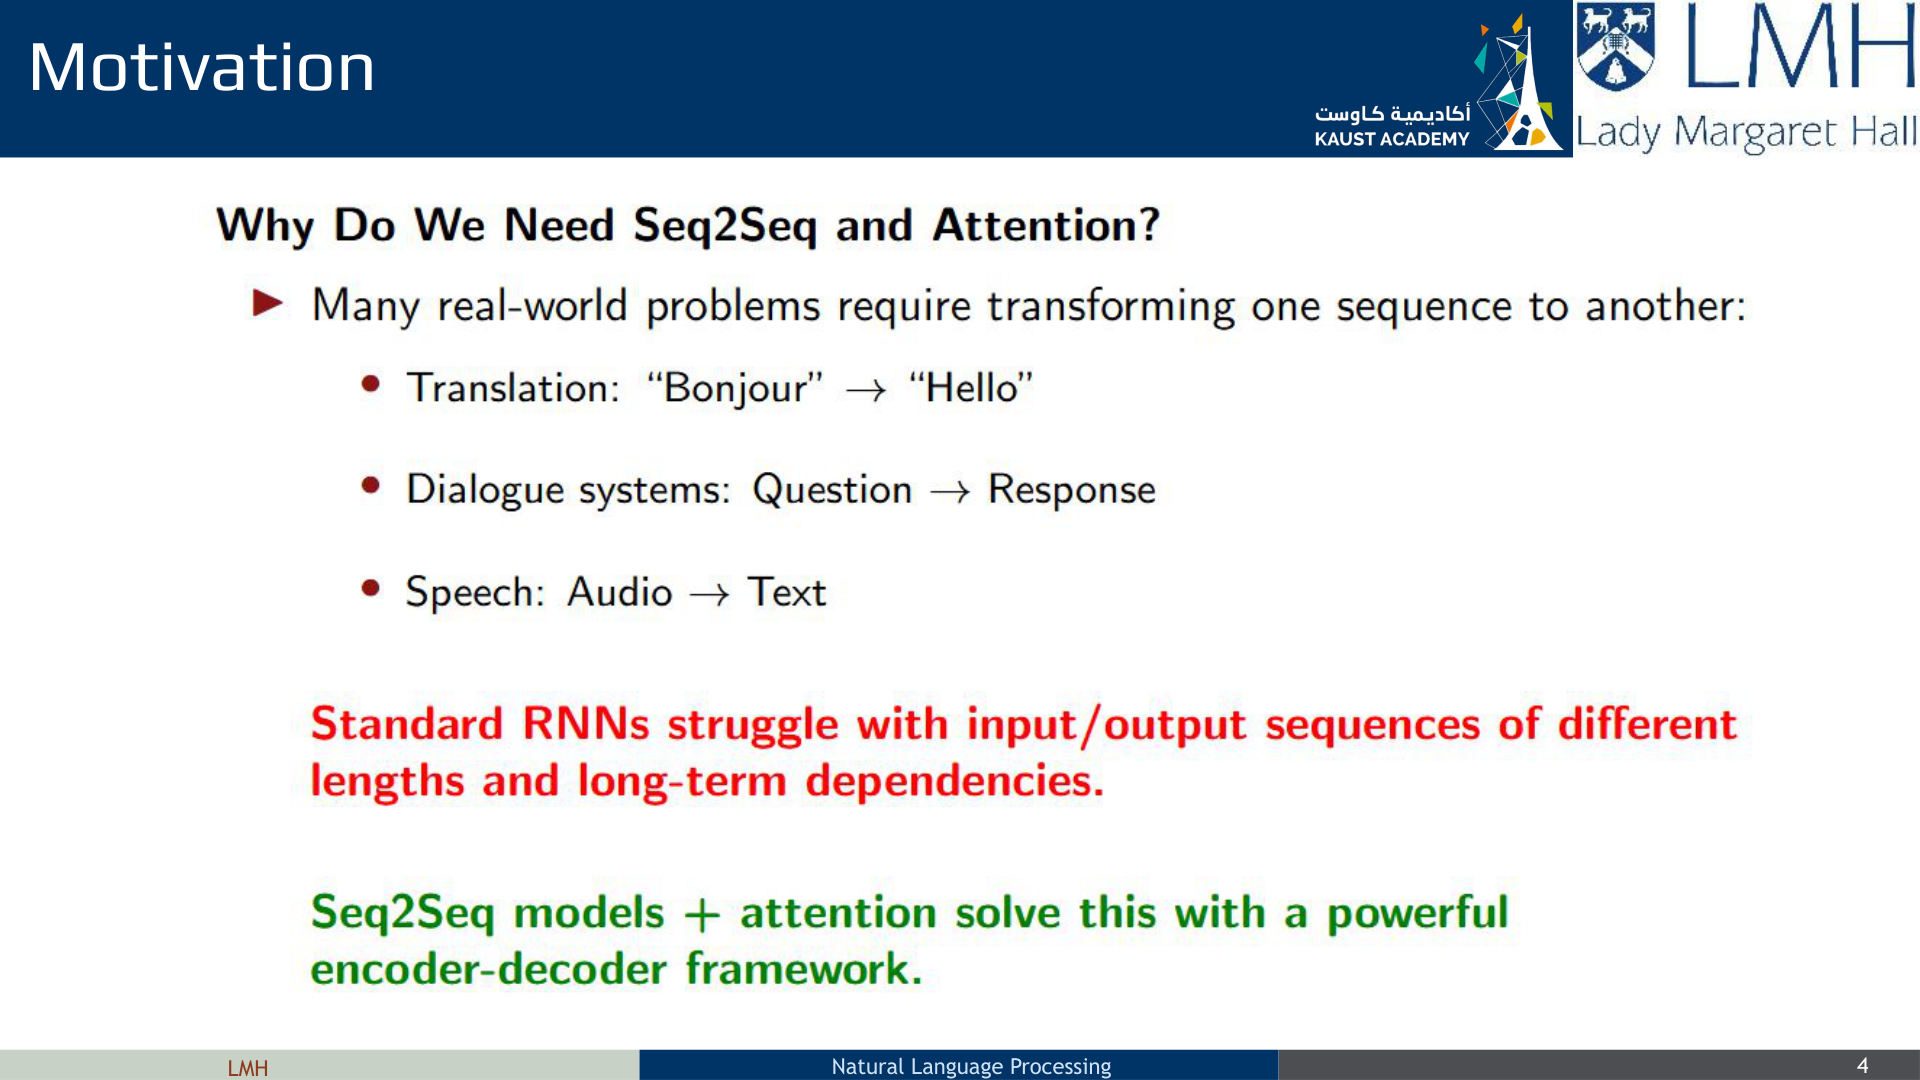
\includegraphics[width=\paperwidth,height=0.95\paperheight,keepaspectratio]{assets/Lecture-11_Large_Reasoning_Models_and_Mixture_of_Experts_Models/pdf_page_004.png}
\end{frame}

\begin{frame}[plain]
  \centering
  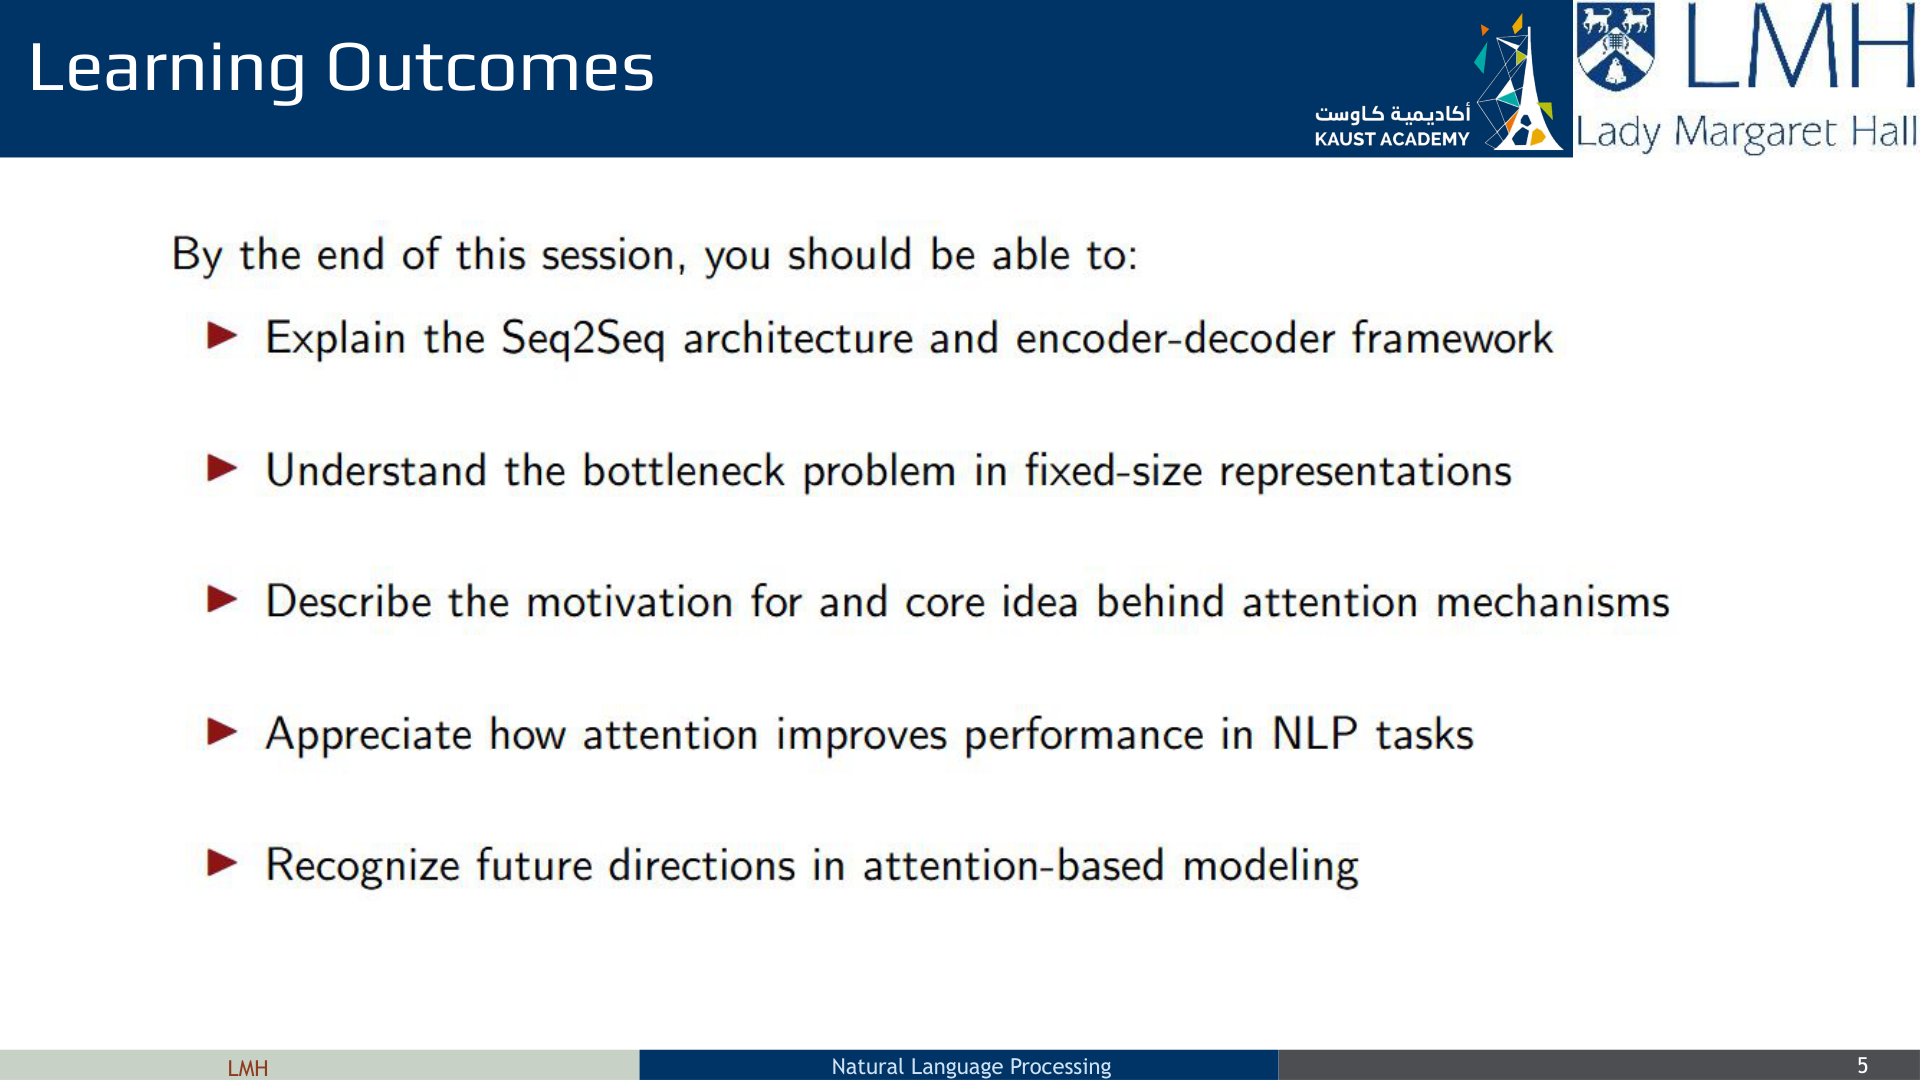
\includegraphics[width=\paperwidth,height=0.95\paperheight,keepaspectratio]{assets/Lecture-11_Large_Reasoning_Models_and_Mixture_of_Experts_Models/pdf_page_005.png}
\end{frame}

\begin{frame}[t]{Natural Language Processing}
  \begin{itemize}
    \item LMH
    \item 6
    \item Seq2Seq Architecture
  \end{itemize}
\end{frame}

\begin{frame}[plain]
  \centering
  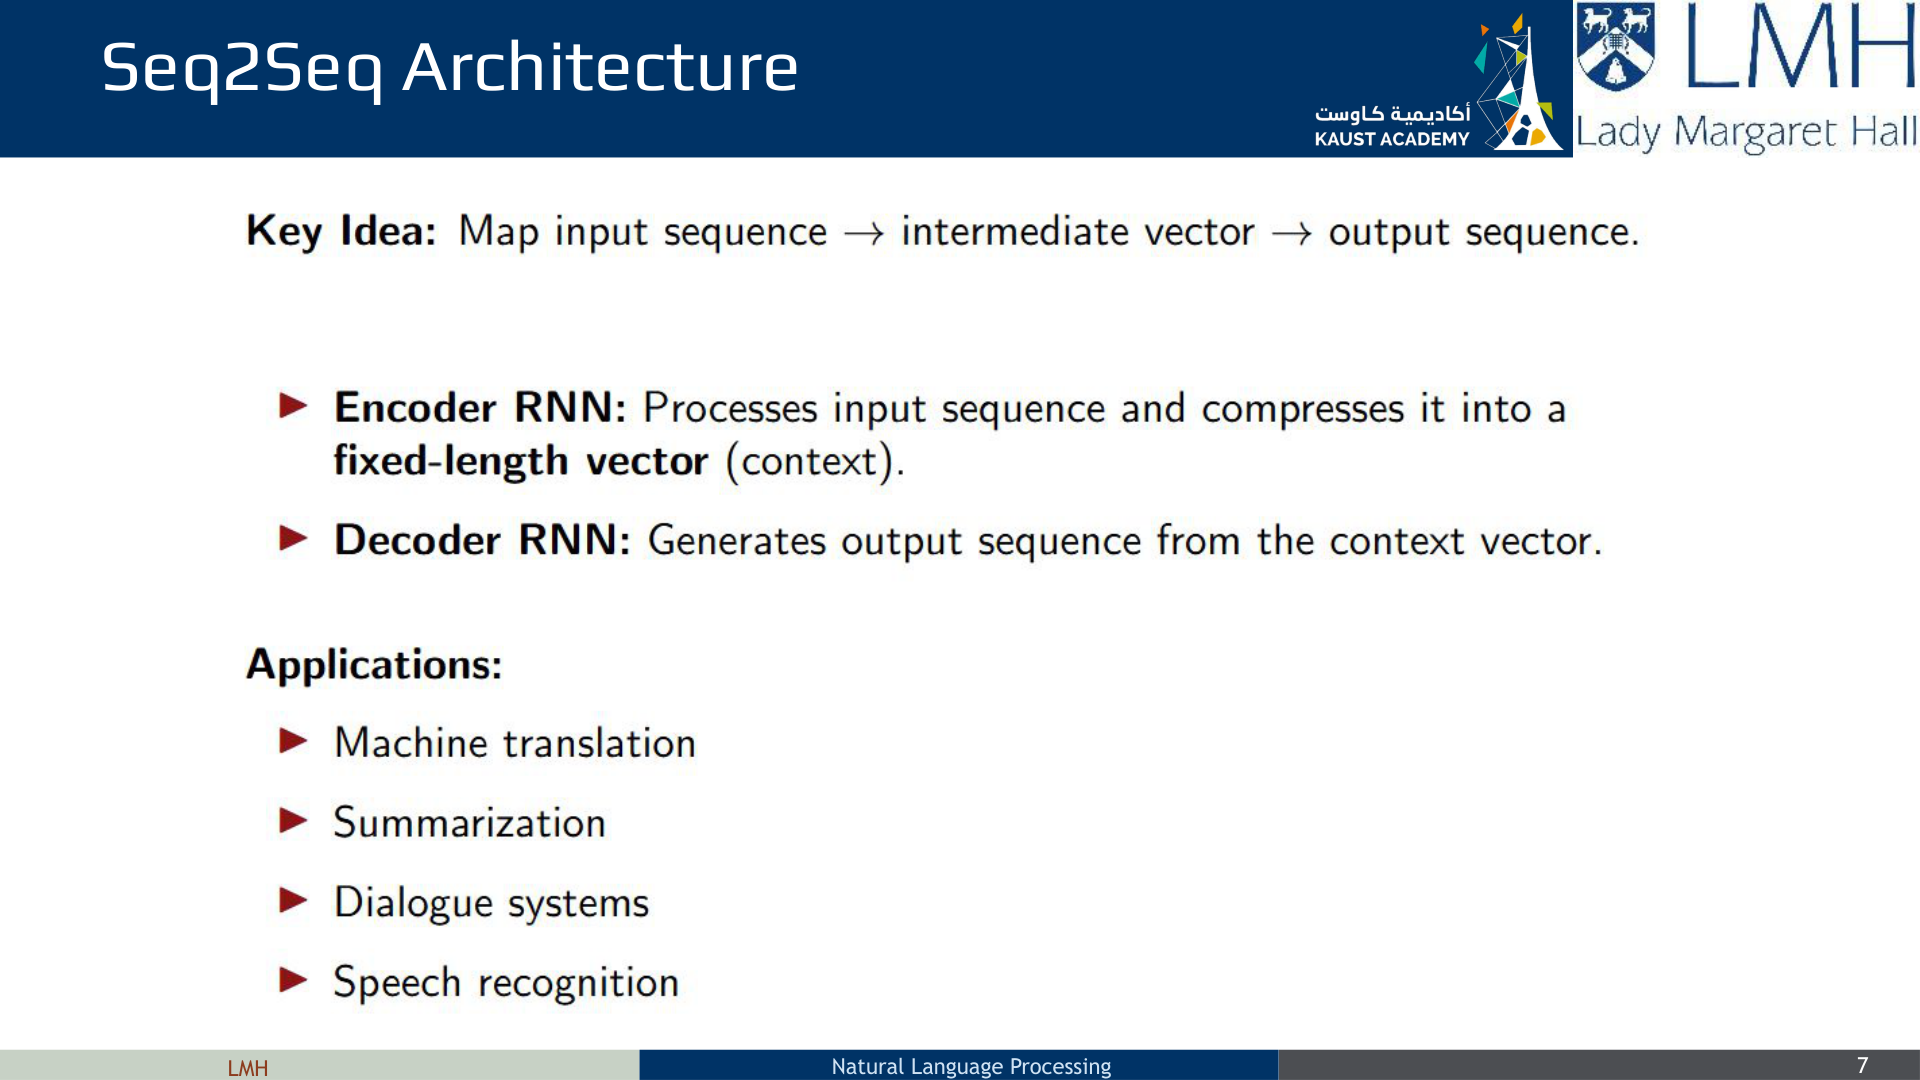
\includegraphics[width=\paperwidth,height=0.95\paperheight,keepaspectratio]{assets/Lecture-11_Large_Reasoning_Models_and_Mixture_of_Experts_Models/pdf_page_007.png}
\end{frame}

\begin{frame}[t]{Natural Language Processing}
  \begin{itemize}
    \item LMH
    \item 8
    \item Seq2Seq Architecture
    \item Seq2seq
    \item Seq2seq
    \item I ate an apple
    \item Ich habe einen apfel gegessen
    \item I ate an apple
    \item - Sequence goes in,
    \item sequence comes out
    \item - No notion of "time synchrony" between input and output
    \item - May even not even maintain order of symbols
    \item - E.g.
    \item "I ate an apple" -> "Ich habe einen apfel gegessen"
    \item v
    \item - Or even seem related to the input
    \item - E.g. "My screen is blank" -> "Please check if your computer is plugged in."
  \end{itemize}
\end{frame}

\begin{frame}[t]{Natural Language Processing}
  \begin{itemize}
    \item LMH
    \item 9
    \item Modelling the problem
    \item ->Delayed sequence to sequence
  \end{itemize}
\end{frame}

\begin{frame}[t]{Natural Language Processing}
  \begin{itemize}
    \item LMH
    \item 10
    \item Modelling the problem
    \item ->Delayed sequence to sequence
    \item First process the input
    \item and generate a hidden
    \item representation for it
  \end{itemize}
\end{frame}

\begin{frame}[t]{Natural Language Processing}
  \begin{itemize}
    \item LMH
    \item 11
    \item Modelling the problem
    \item ->Delayed sequence to sequence
    \item First process the input
    \item and generate a hidden
    \item representation for it
    \item Then use it to generate
    \item an output
  \end{itemize}
\end{frame}

\begin{frame}[t]{Natural Language Processing}
  \begin{itemize}
    \item LMH
    \item 12
    \item Modelling the problem
    \item ->Problem: Each word that is output depends only on
    \item current hidden state, and not on previous outputs
    \item First process the input
    \item and generate a hidden
    \item representation for it
    \item Then use it to generate
    \item an output
  \end{itemize}
\end{frame}

\begin{frame}[t]{Natural Language Processing}
  \begin{itemize}
    \item LMH
    \item 13
    \item Modelling the problem
    \item ->Delayed sequence to sequence
    \item oDelayed self-referencing sequence-to-sequence
  \end{itemize}
\end{frame}

\begin{frame}[plain]
  \centering
  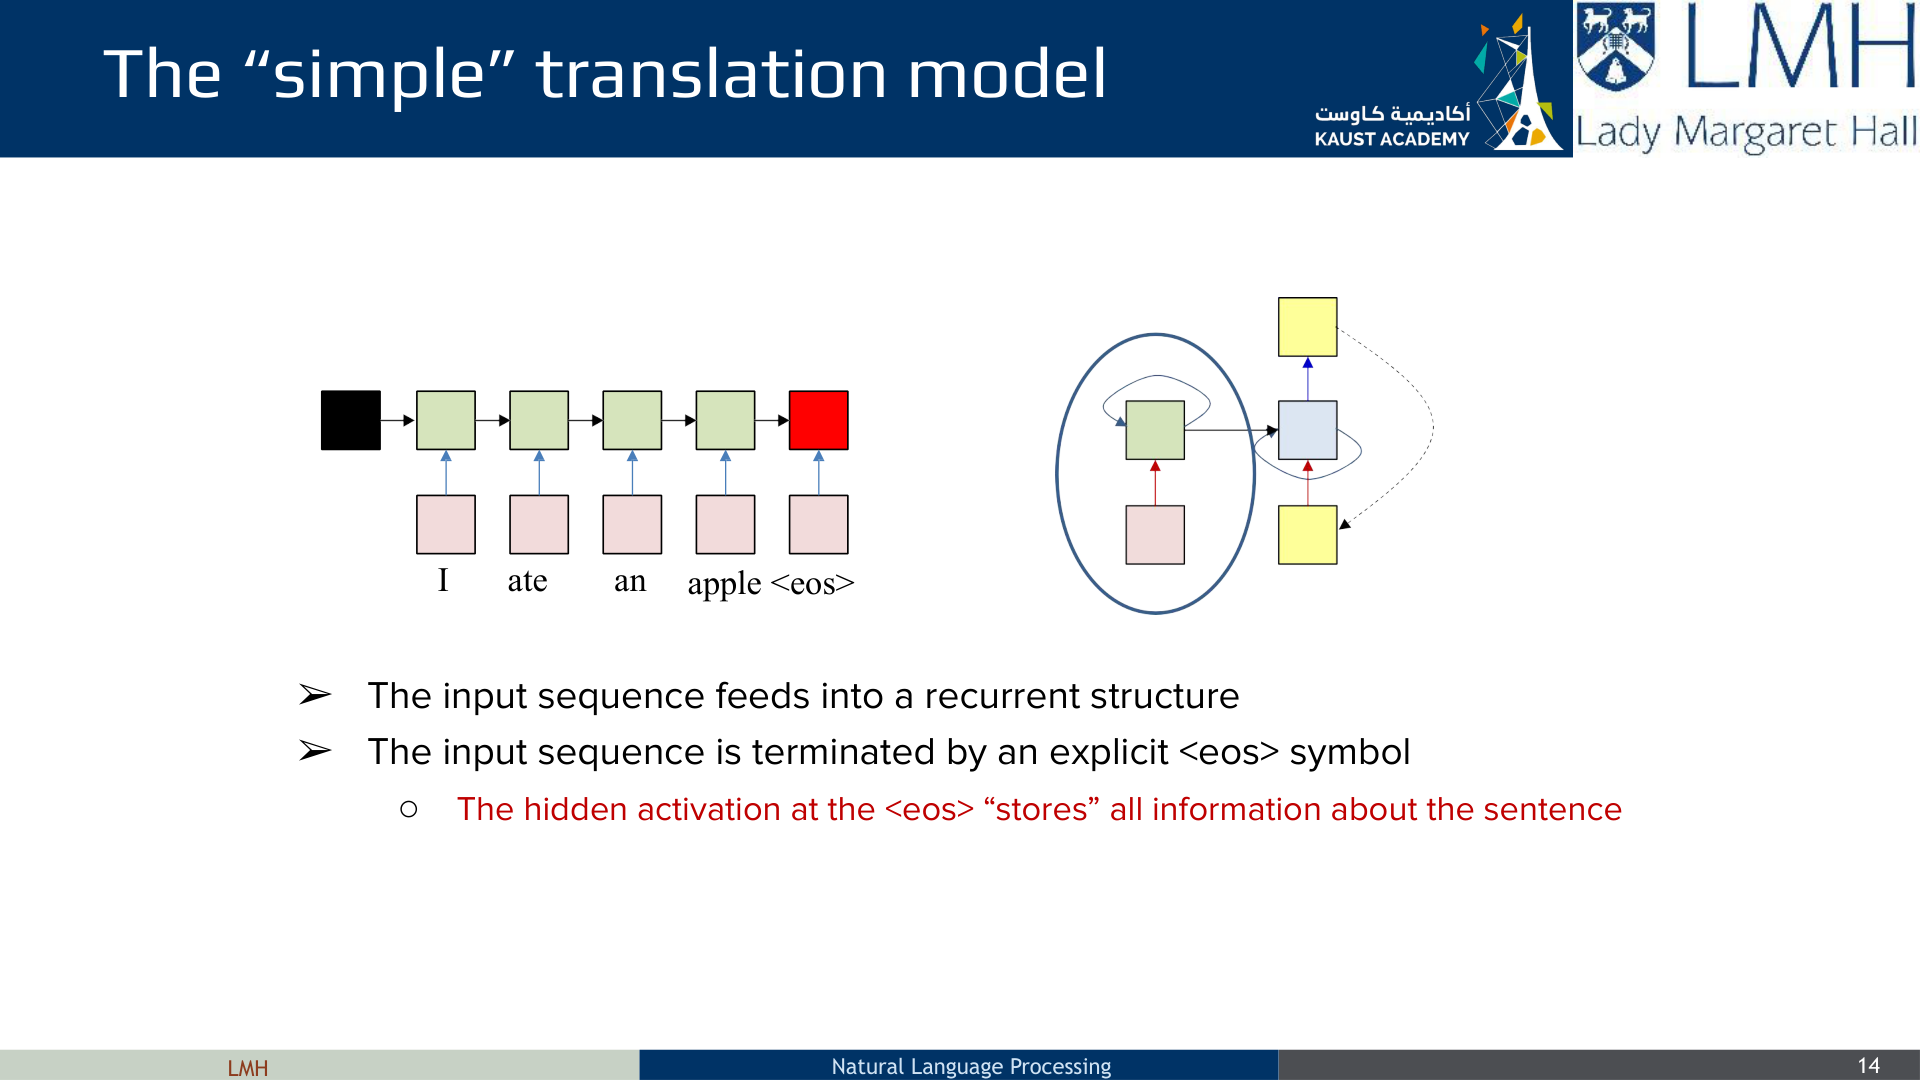
\includegraphics[width=\paperwidth,height=0.95\paperheight,keepaspectratio]{assets/Lecture-11_Large_Reasoning_Models_and_Mixture_of_Experts_Models/pdf_page_014.png}
\end{frame}

\begin{frame}[plain]
  \centering
  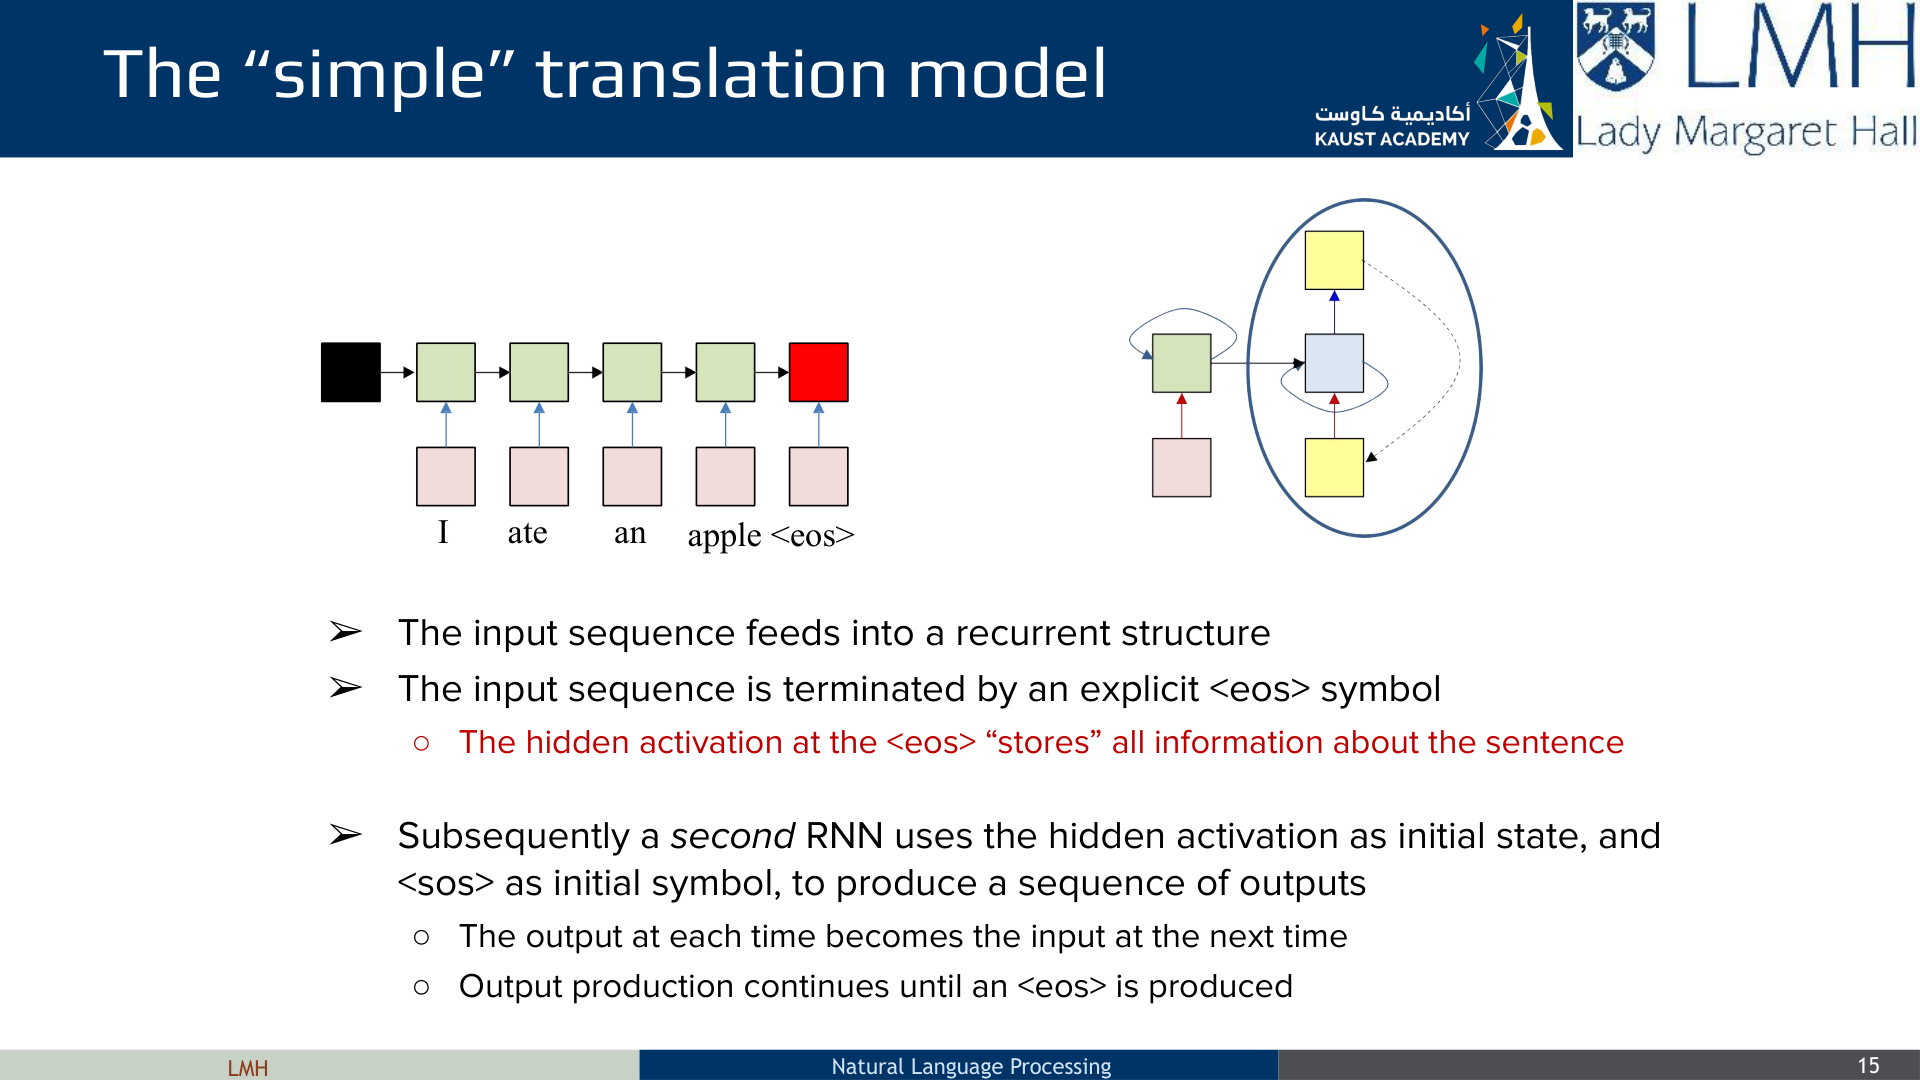
\includegraphics[width=\paperwidth,height=0.95\paperheight,keepaspectratio]{assets/Lecture-11_Large_Reasoning_Models_and_Mixture_of_Experts_Models/pdf_page_015.png}
\end{frame}

\begin{frame}[plain]
  \centering
  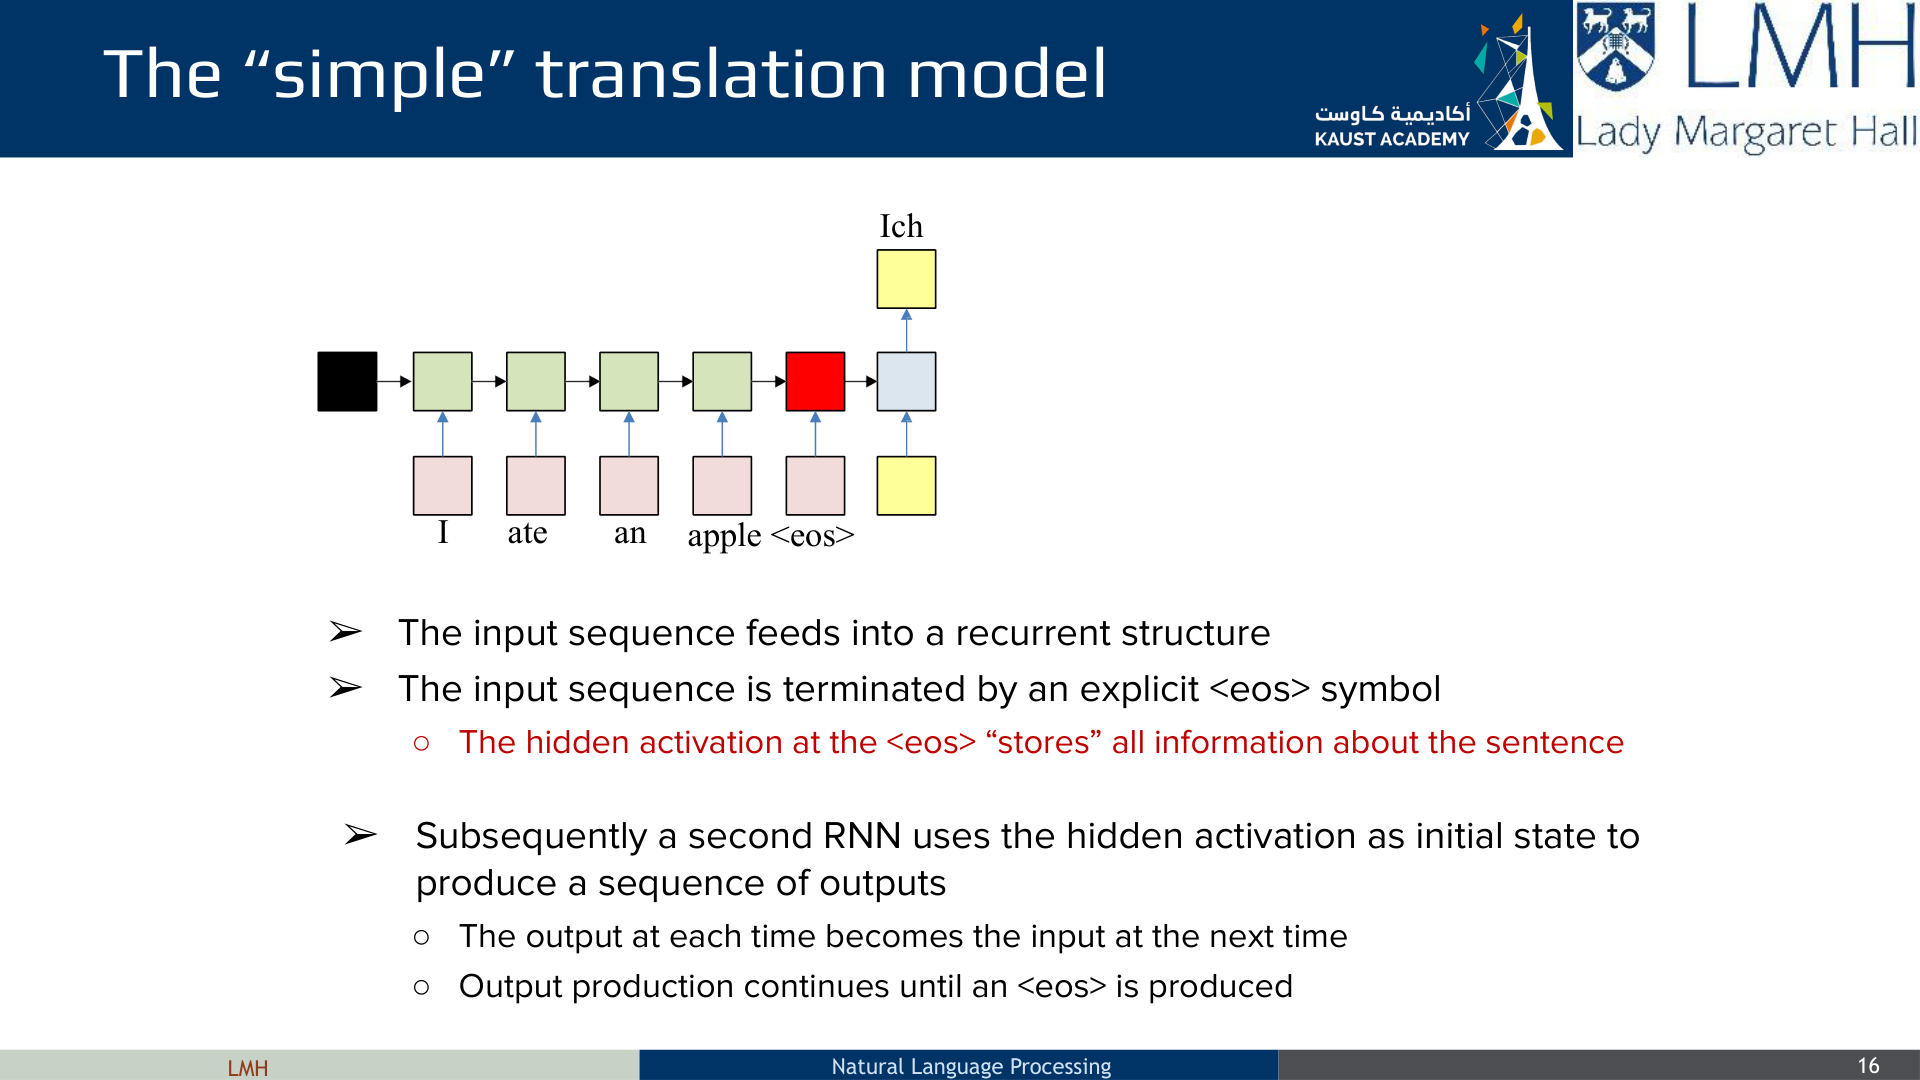
\includegraphics[width=\paperwidth,height=0.95\paperheight,keepaspectratio]{assets/Lecture-11_Large_Reasoning_Models_and_Mixture_of_Experts_Models/pdf_page_016.png}
\end{frame}

\begin{frame}[plain]
  \centering
  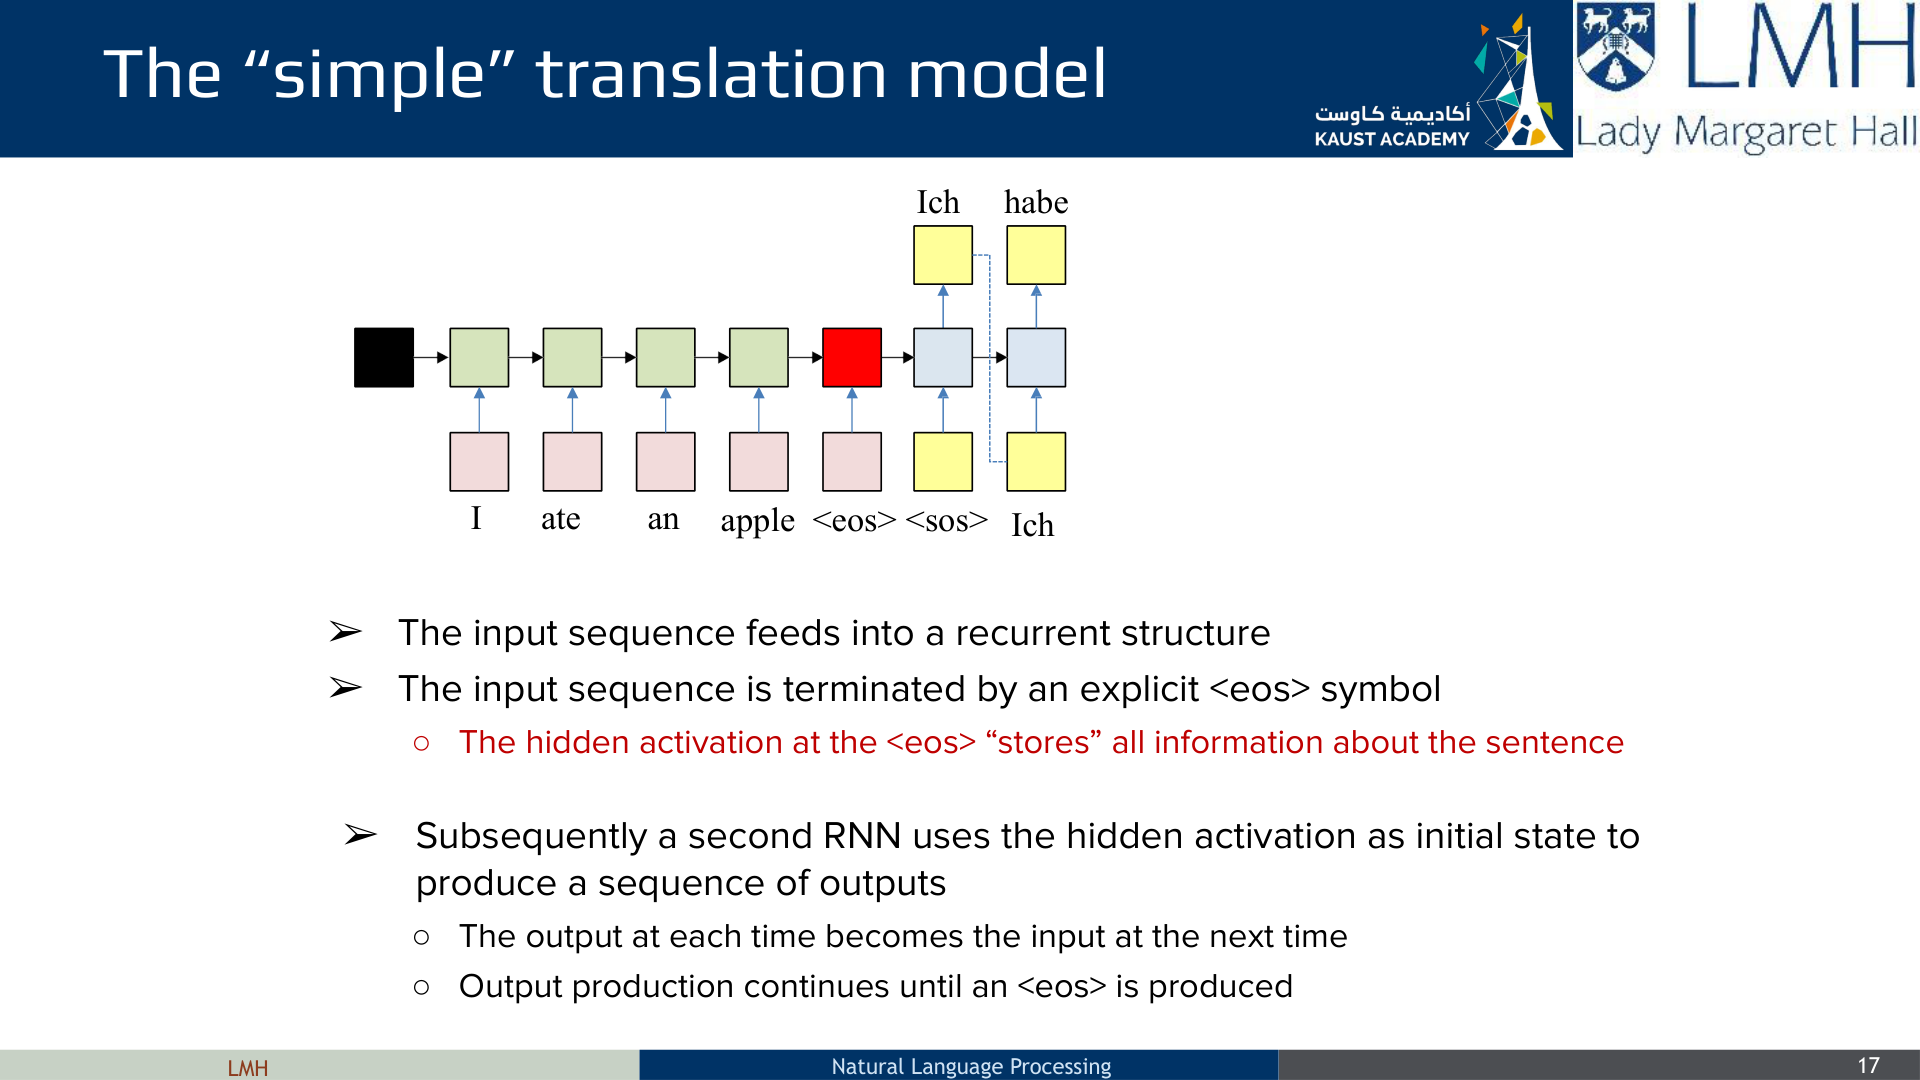
\includegraphics[width=\paperwidth,height=0.95\paperheight,keepaspectratio]{assets/Lecture-11_Large_Reasoning_Models_and_Mixture_of_Experts_Models/pdf_page_017.png}
\end{frame}

\begin{frame}[plain]
  \centering
  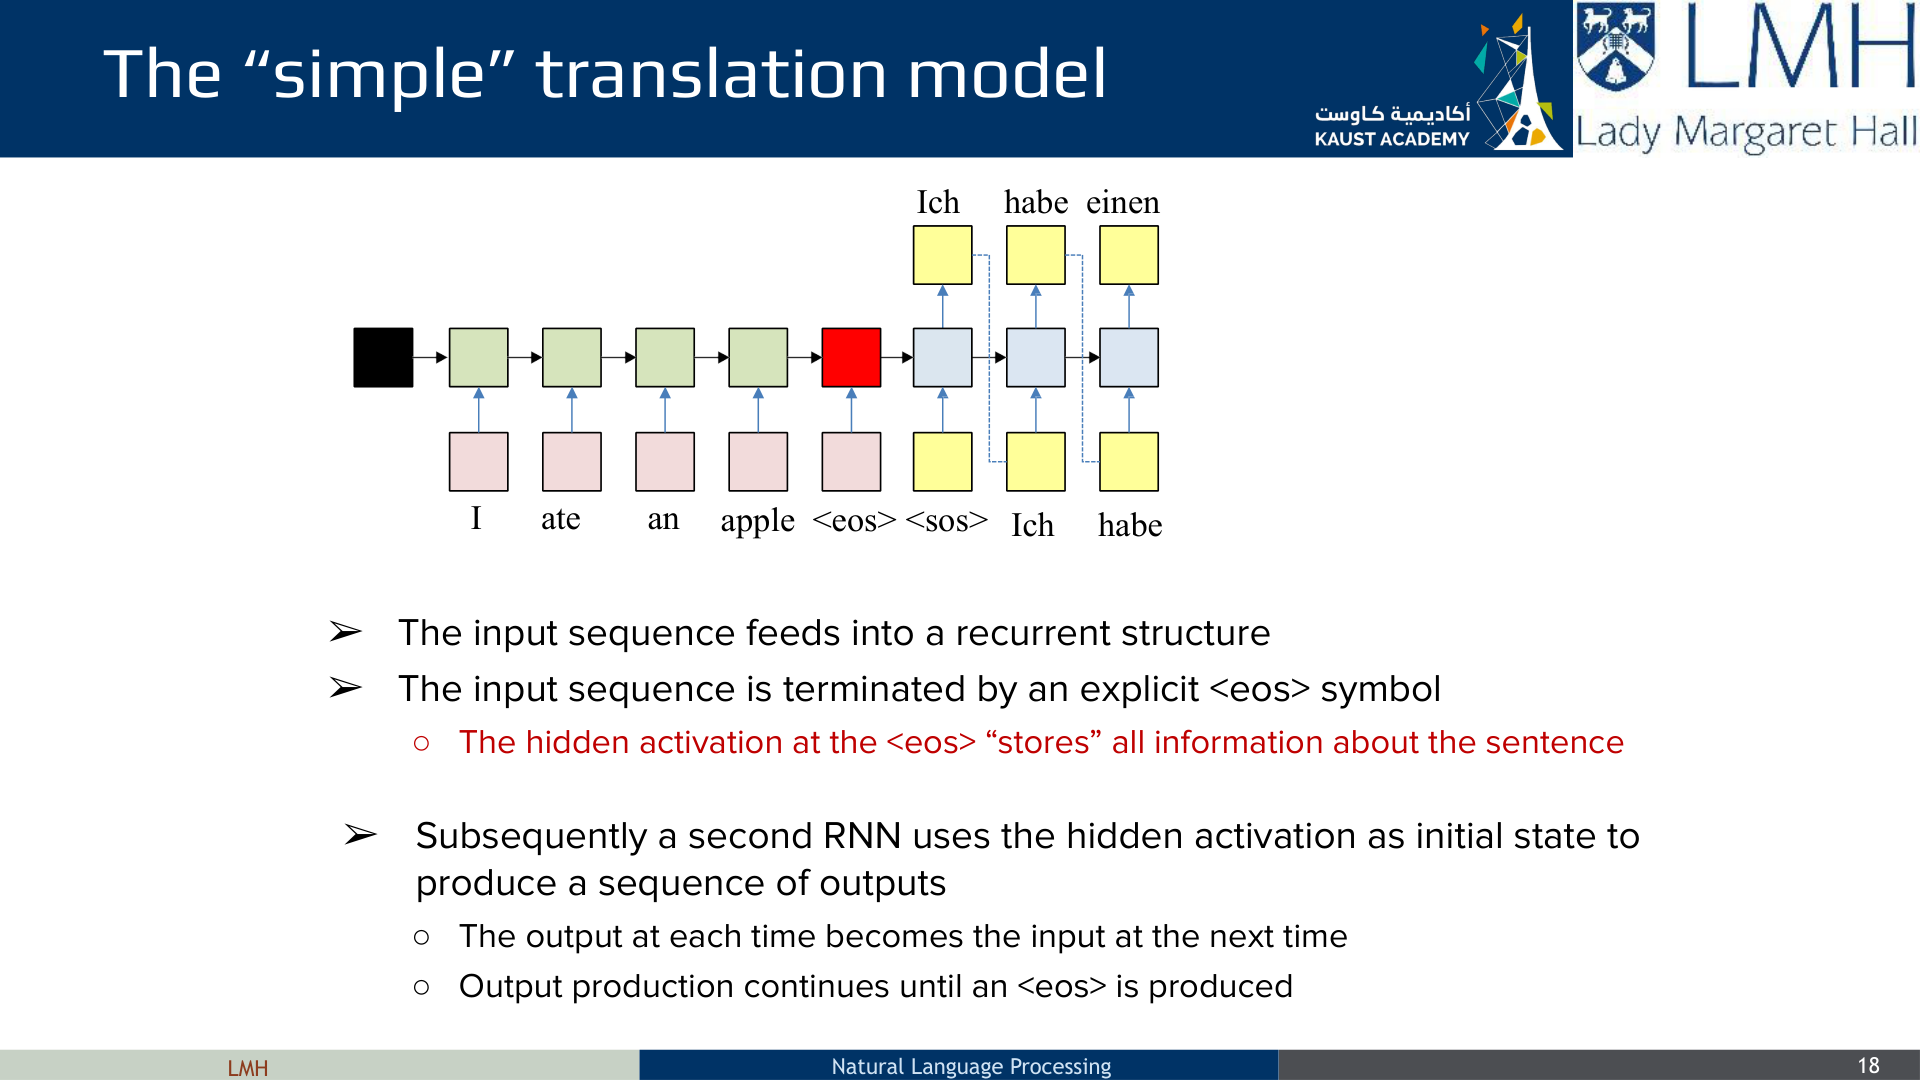
\includegraphics[width=\paperwidth,height=0.95\paperheight,keepaspectratio]{assets/Lecture-11_Large_Reasoning_Models_and_Mixture_of_Experts_Models/pdf_page_018.png}
\end{frame}

\begin{frame}[plain]
  \centering
  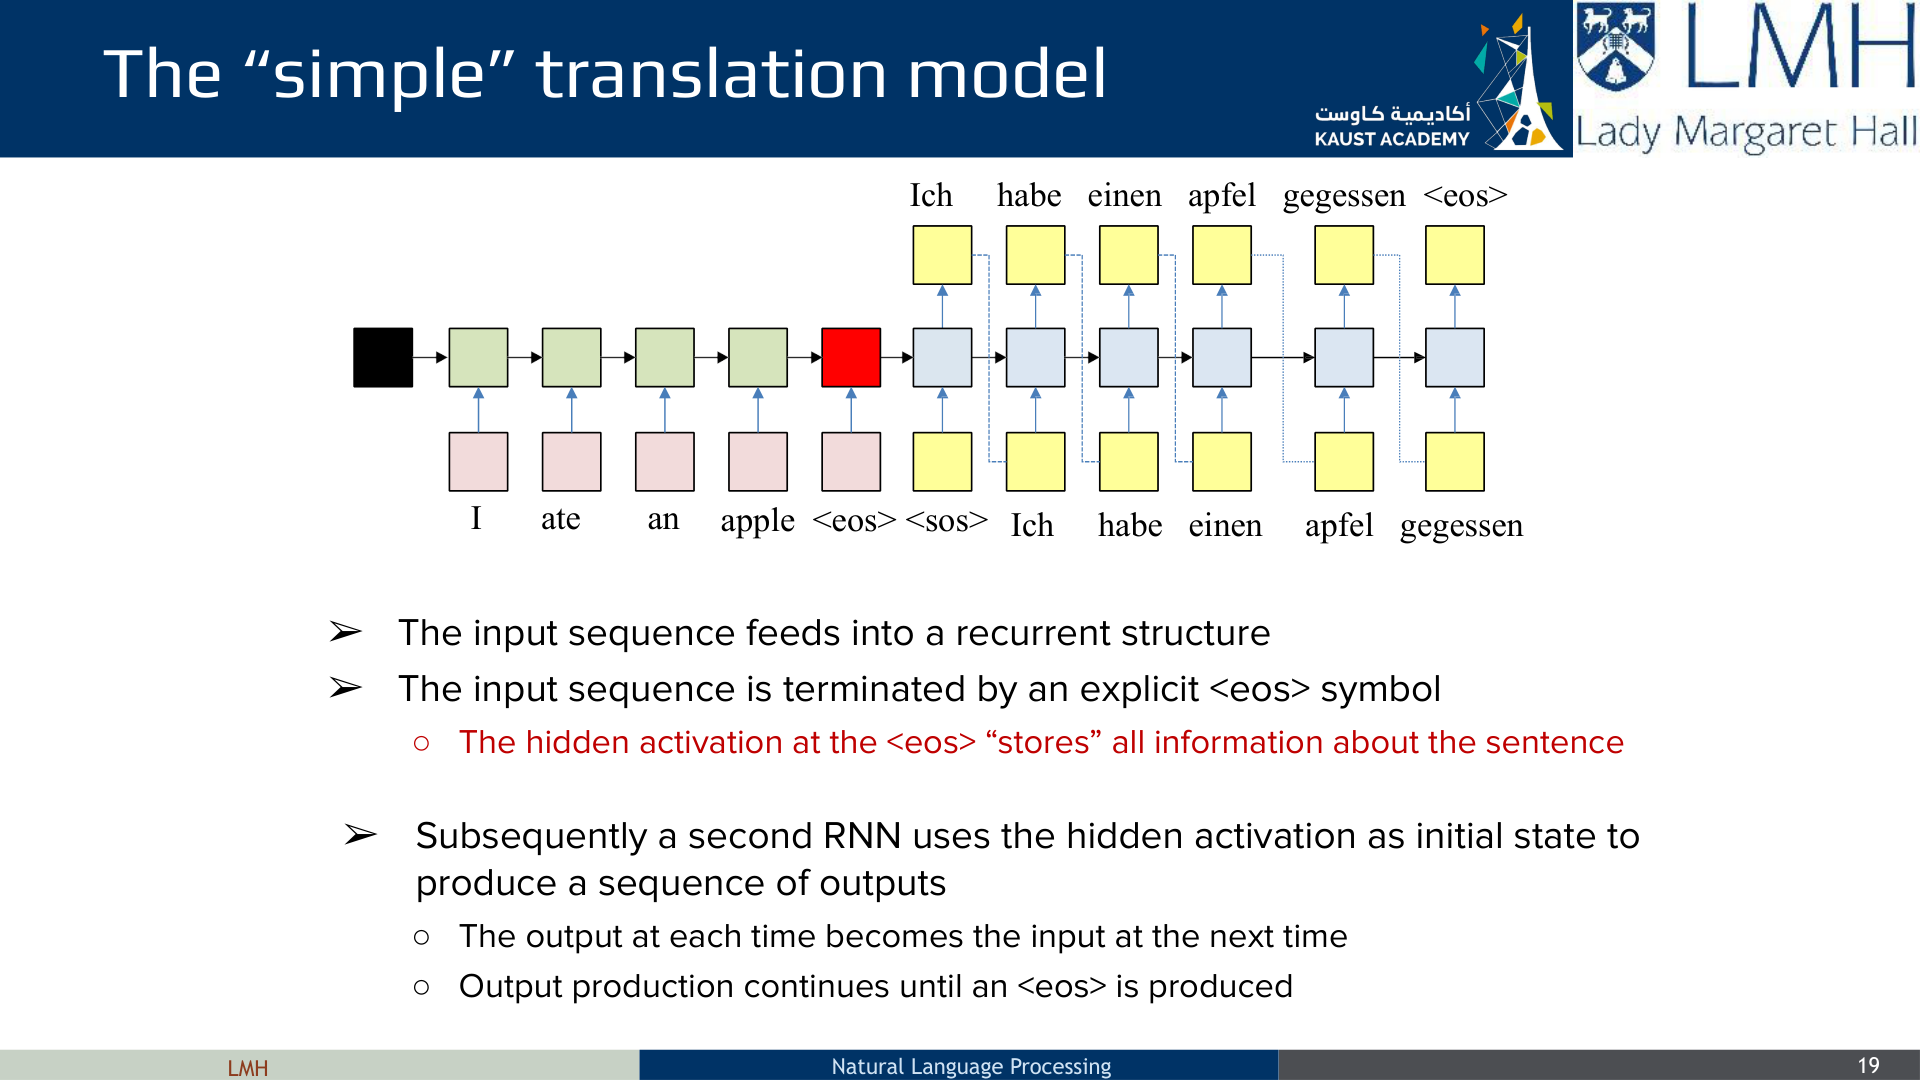
\includegraphics[width=\paperwidth,height=0.95\paperheight,keepaspectratio]{assets/Lecture-11_Large_Reasoning_Models_and_Mixture_of_Experts_Models/pdf_page_019.png}
\end{frame}

\begin{frame}[plain]
  \centering
  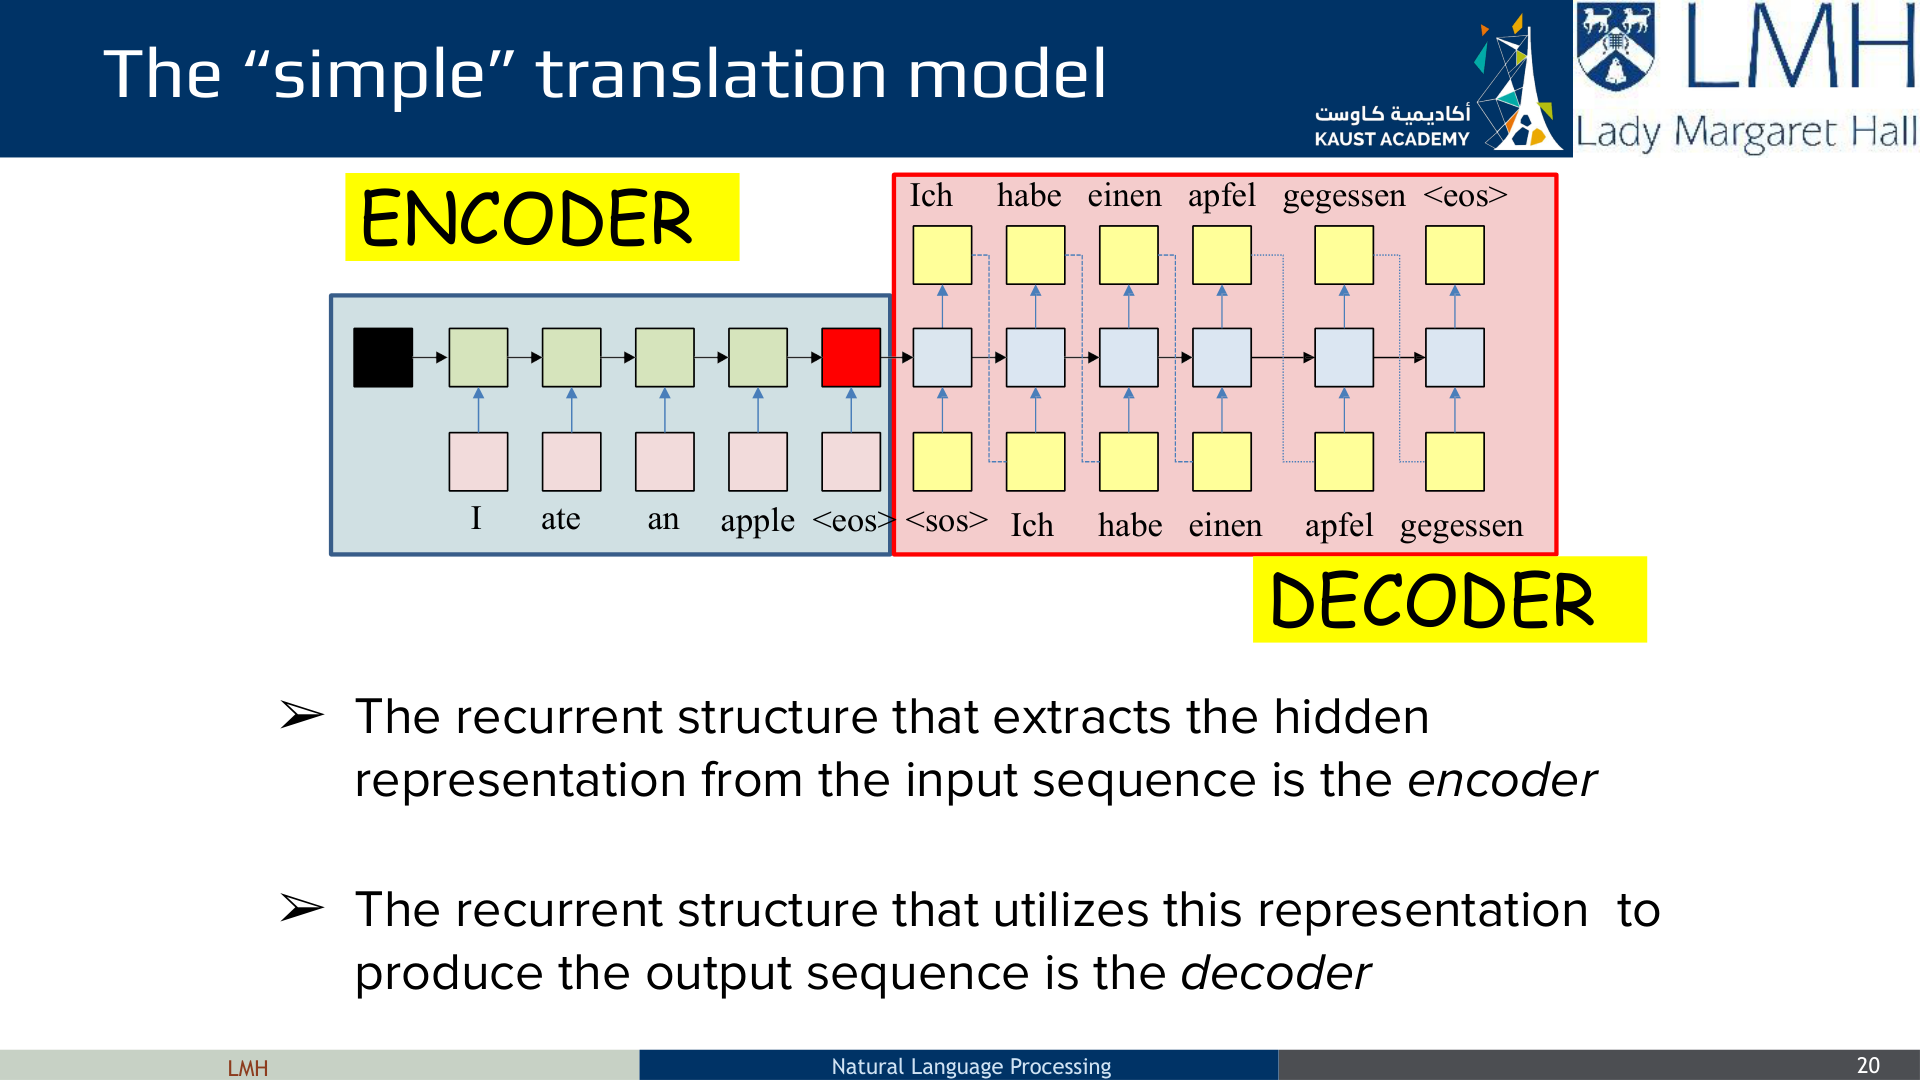
\includegraphics[width=\paperwidth,height=0.95\paperheight,keepaspectratio]{assets/Lecture-11_Large_Reasoning_Models_and_Mixture_of_Experts_Models/pdf_page_020.png}
\end{frame}

\begin{frame}[t]{Natural Language Processing}
  \begin{itemize}
    \item LMH
    \item 21
    \item The Bottleneck Problem
  \end{itemize}
\end{frame}

\begin{frame}[plain]
  \centering
  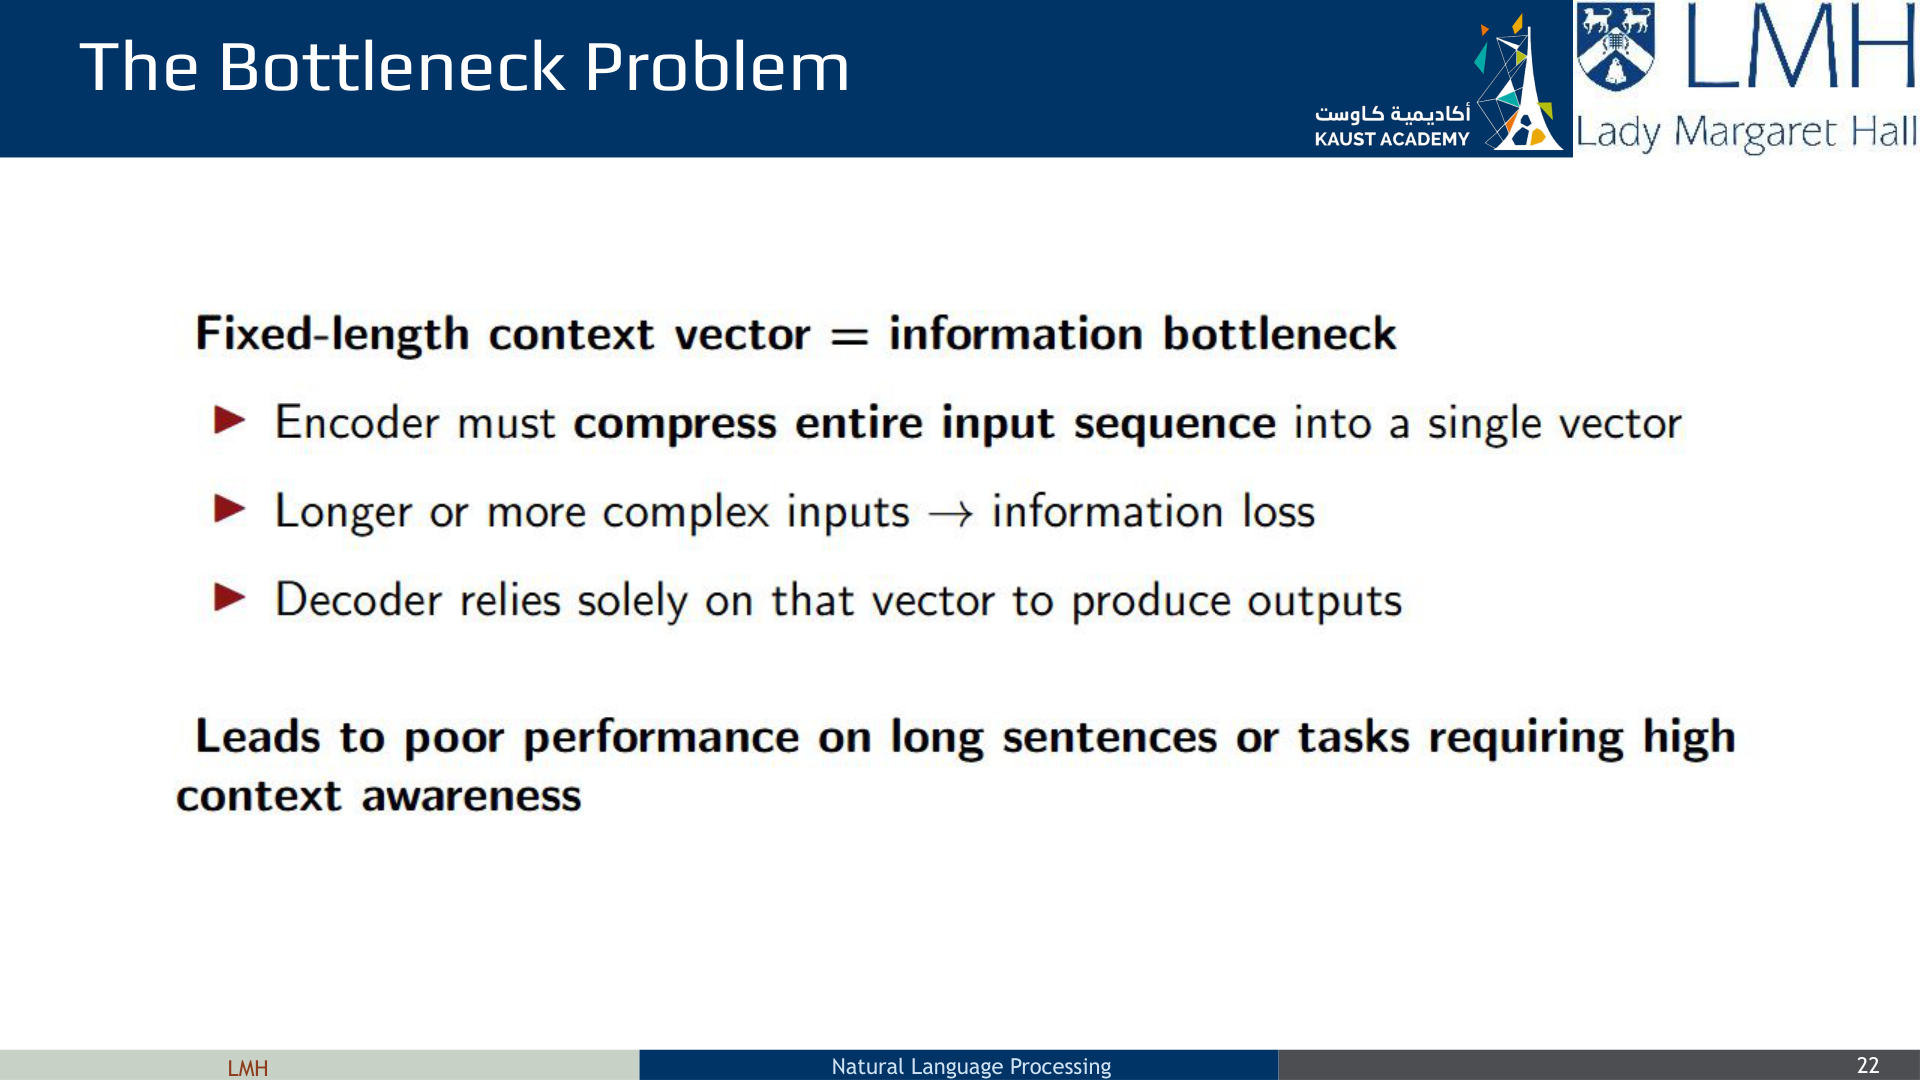
\includegraphics[width=\paperwidth,height=0.95\paperheight,keepaspectratio]{assets/Lecture-11_Large_Reasoning_Models_and_Mixture_of_Experts_Models/pdf_page_022.png}
\end{frame}

\begin{frame}[plain]
  \centering
  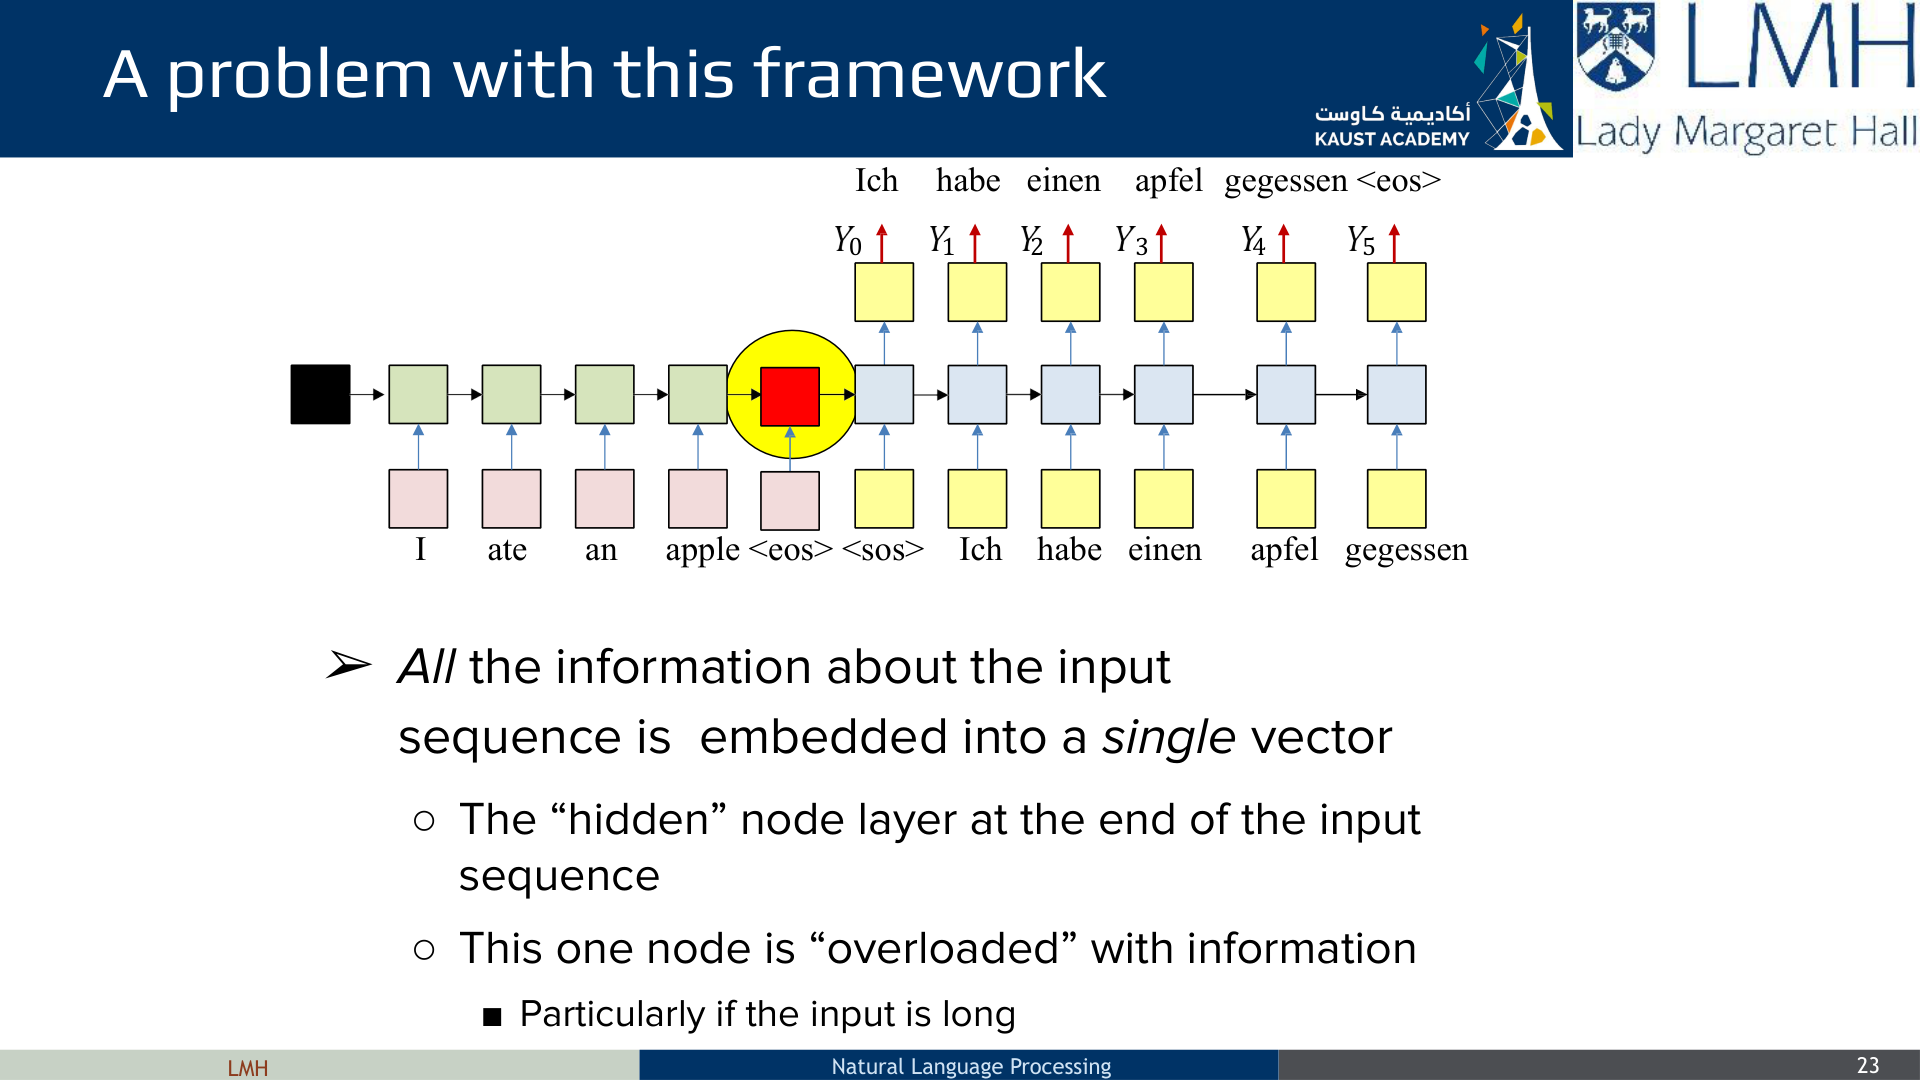
\includegraphics[width=\paperwidth,height=0.95\paperheight,keepaspectratio]{assets/Lecture-11_Large_Reasoning_Models_and_Mixture_of_Experts_Models/pdf_page_023.png}
\end{frame}

\begin{frame}[plain]
  \centering
  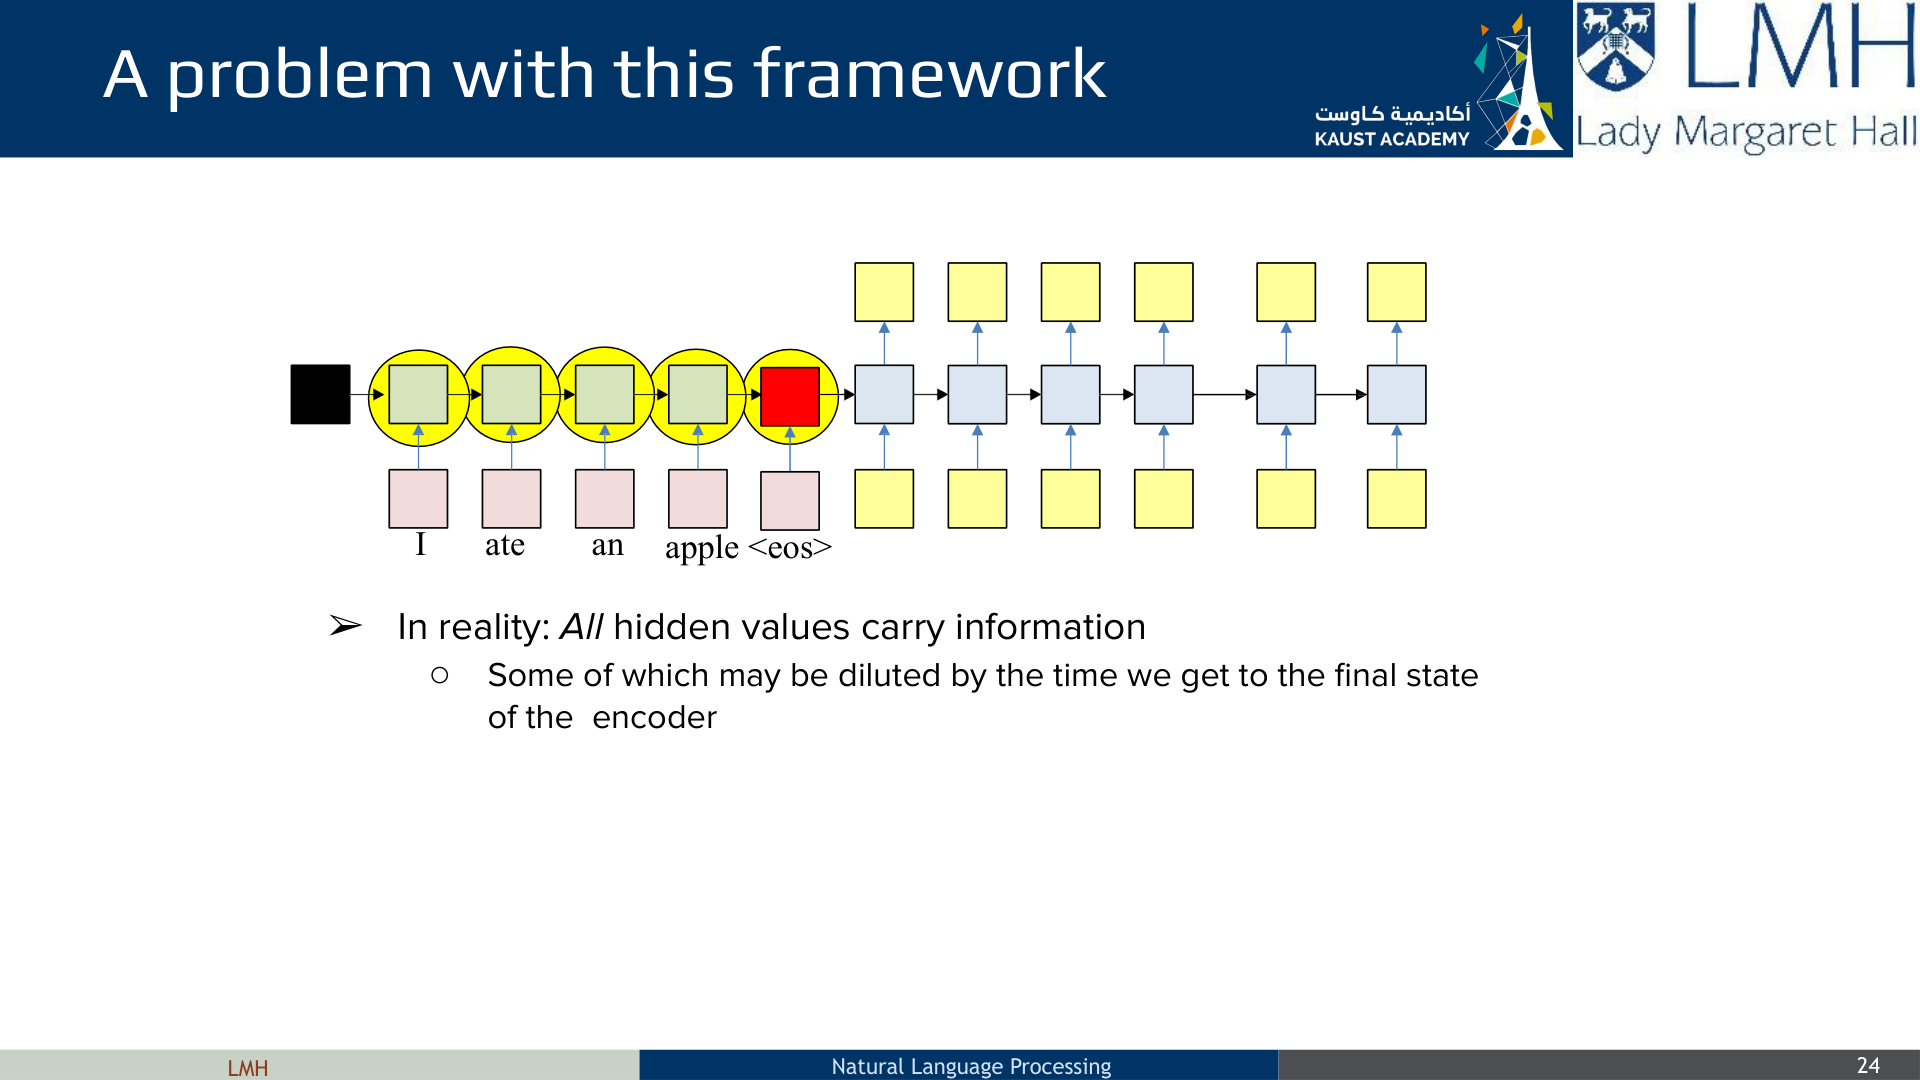
\includegraphics[width=\paperwidth,height=0.95\paperheight,keepaspectratio]{assets/Lecture-11_Large_Reasoning_Models_and_Mixture_of_Experts_Models/pdf_page_024.png}
\end{frame}

\begin{frame}[plain]
  \centering
  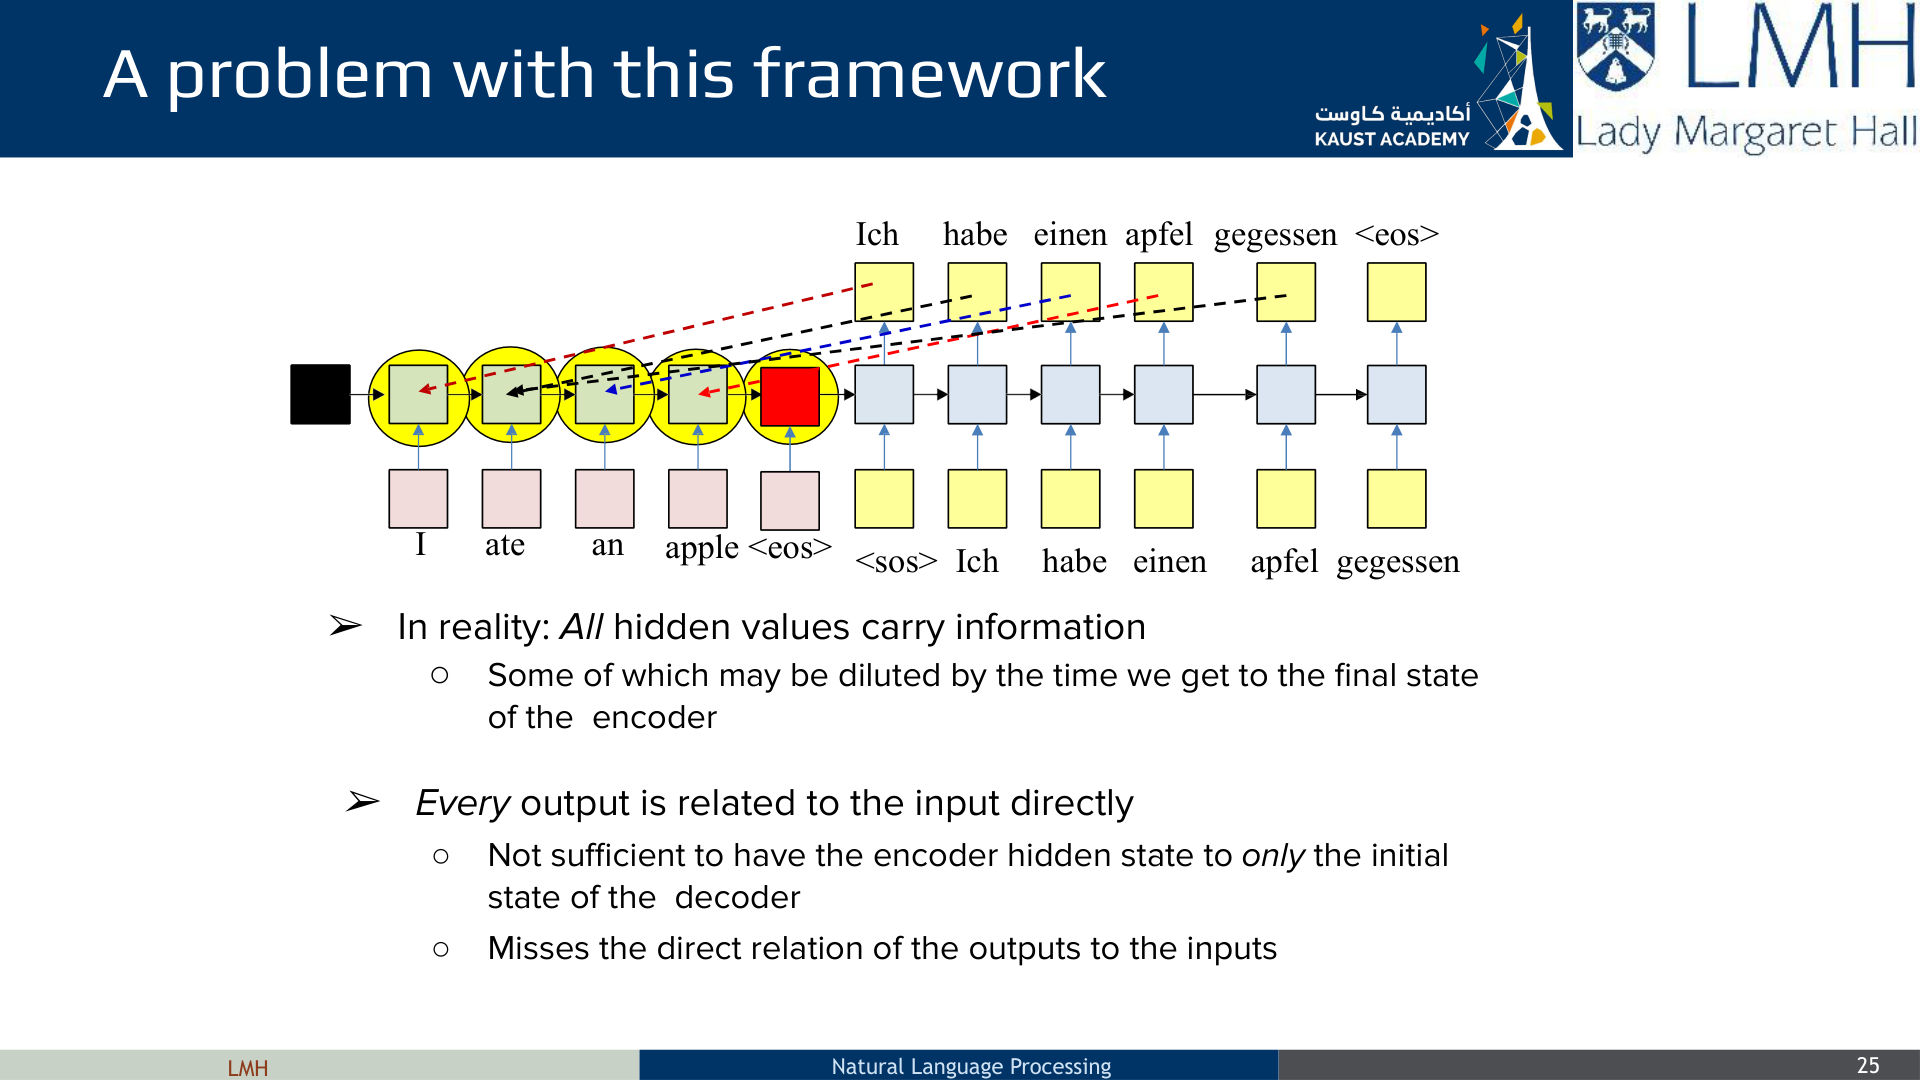
\includegraphics[width=\paperwidth,height=0.95\paperheight,keepaspectratio]{assets/Lecture-11_Large_Reasoning_Models_and_Mixture_of_Experts_Models/pdf_page_025.png}
\end{frame}

\begin{frame}[t]{Natural Language Processing}
  \begin{itemize}
    \item LMH
    \item 26
    \item Realization: We Need More Context!
  \end{itemize}
\end{frame}

\begin{frame}[plain]
  \centering
  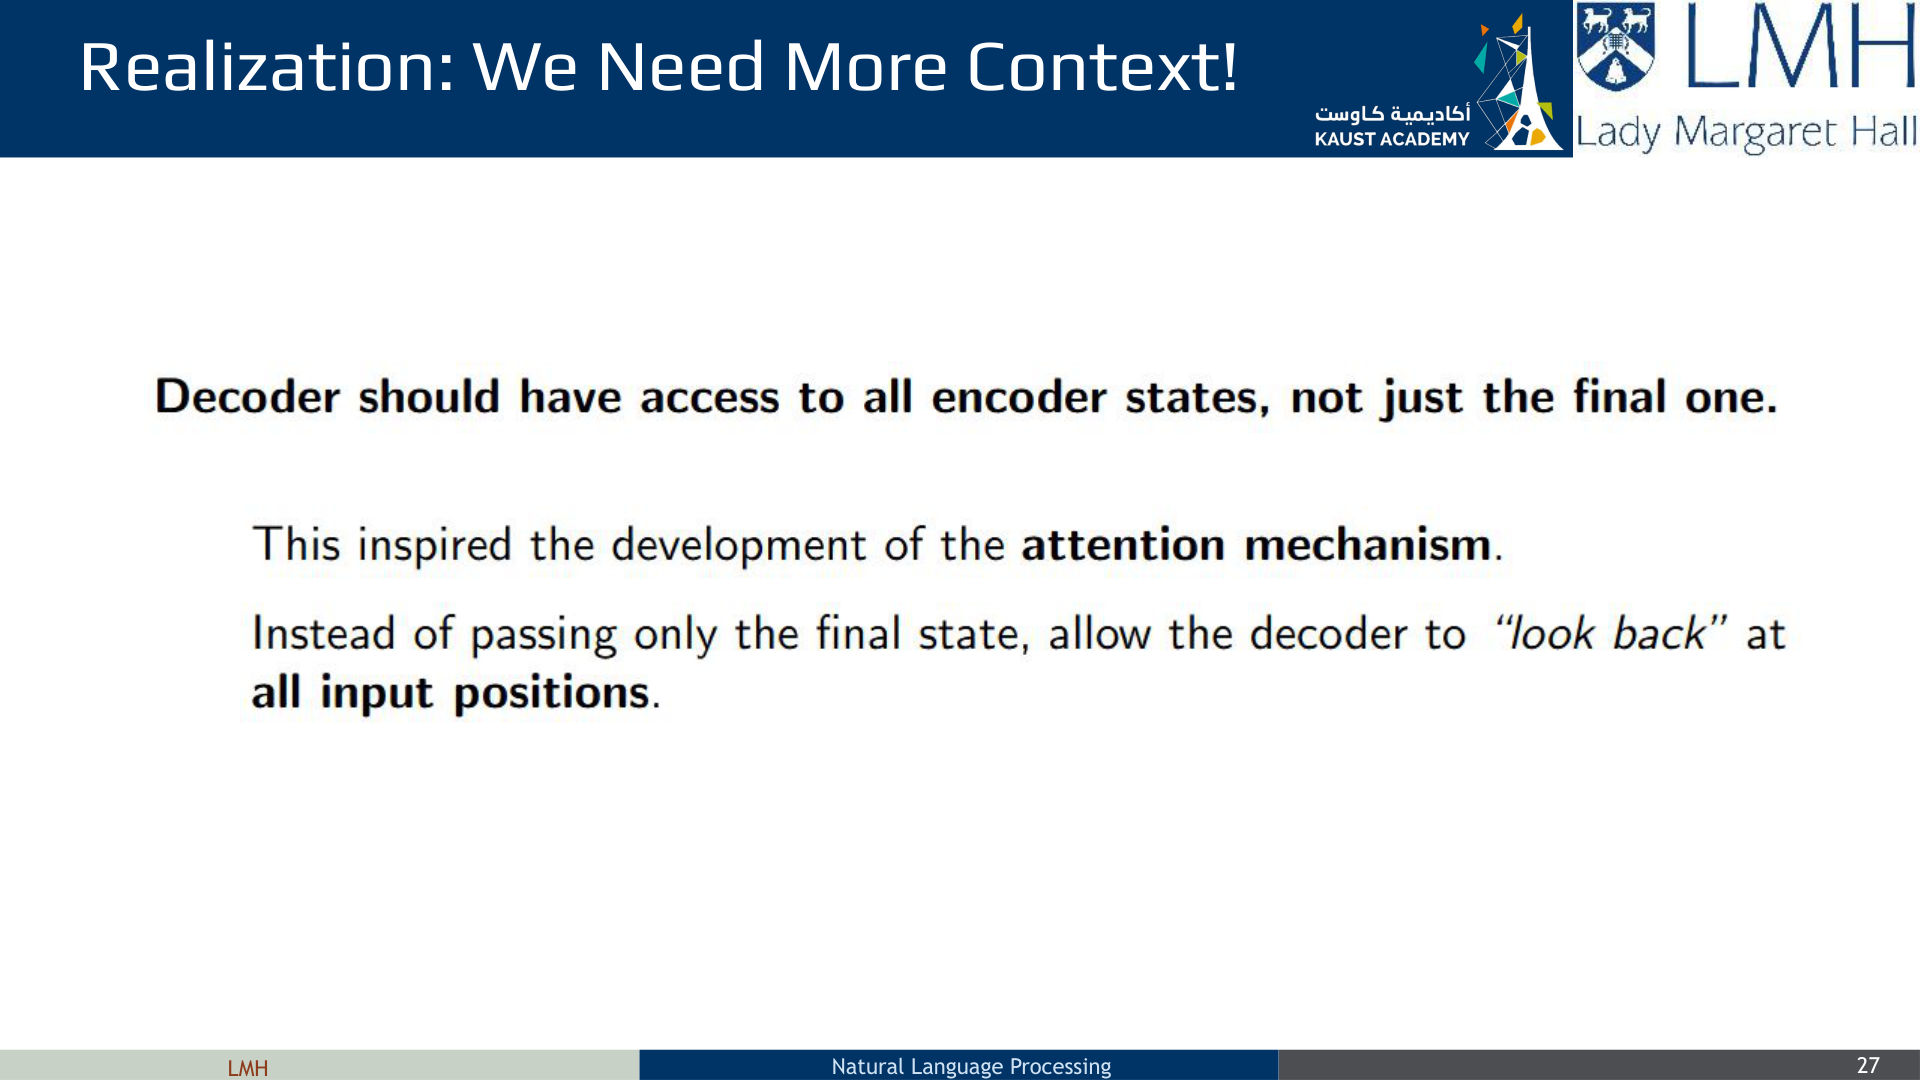
\includegraphics[width=\paperwidth,height=0.95\paperheight,keepaspectratio]{assets/Lecture-11_Large_Reasoning_Models_and_Mixture_of_Experts_Models/pdf_page_027.png}
\end{frame}

\begin{frame}[plain]
  \centering
  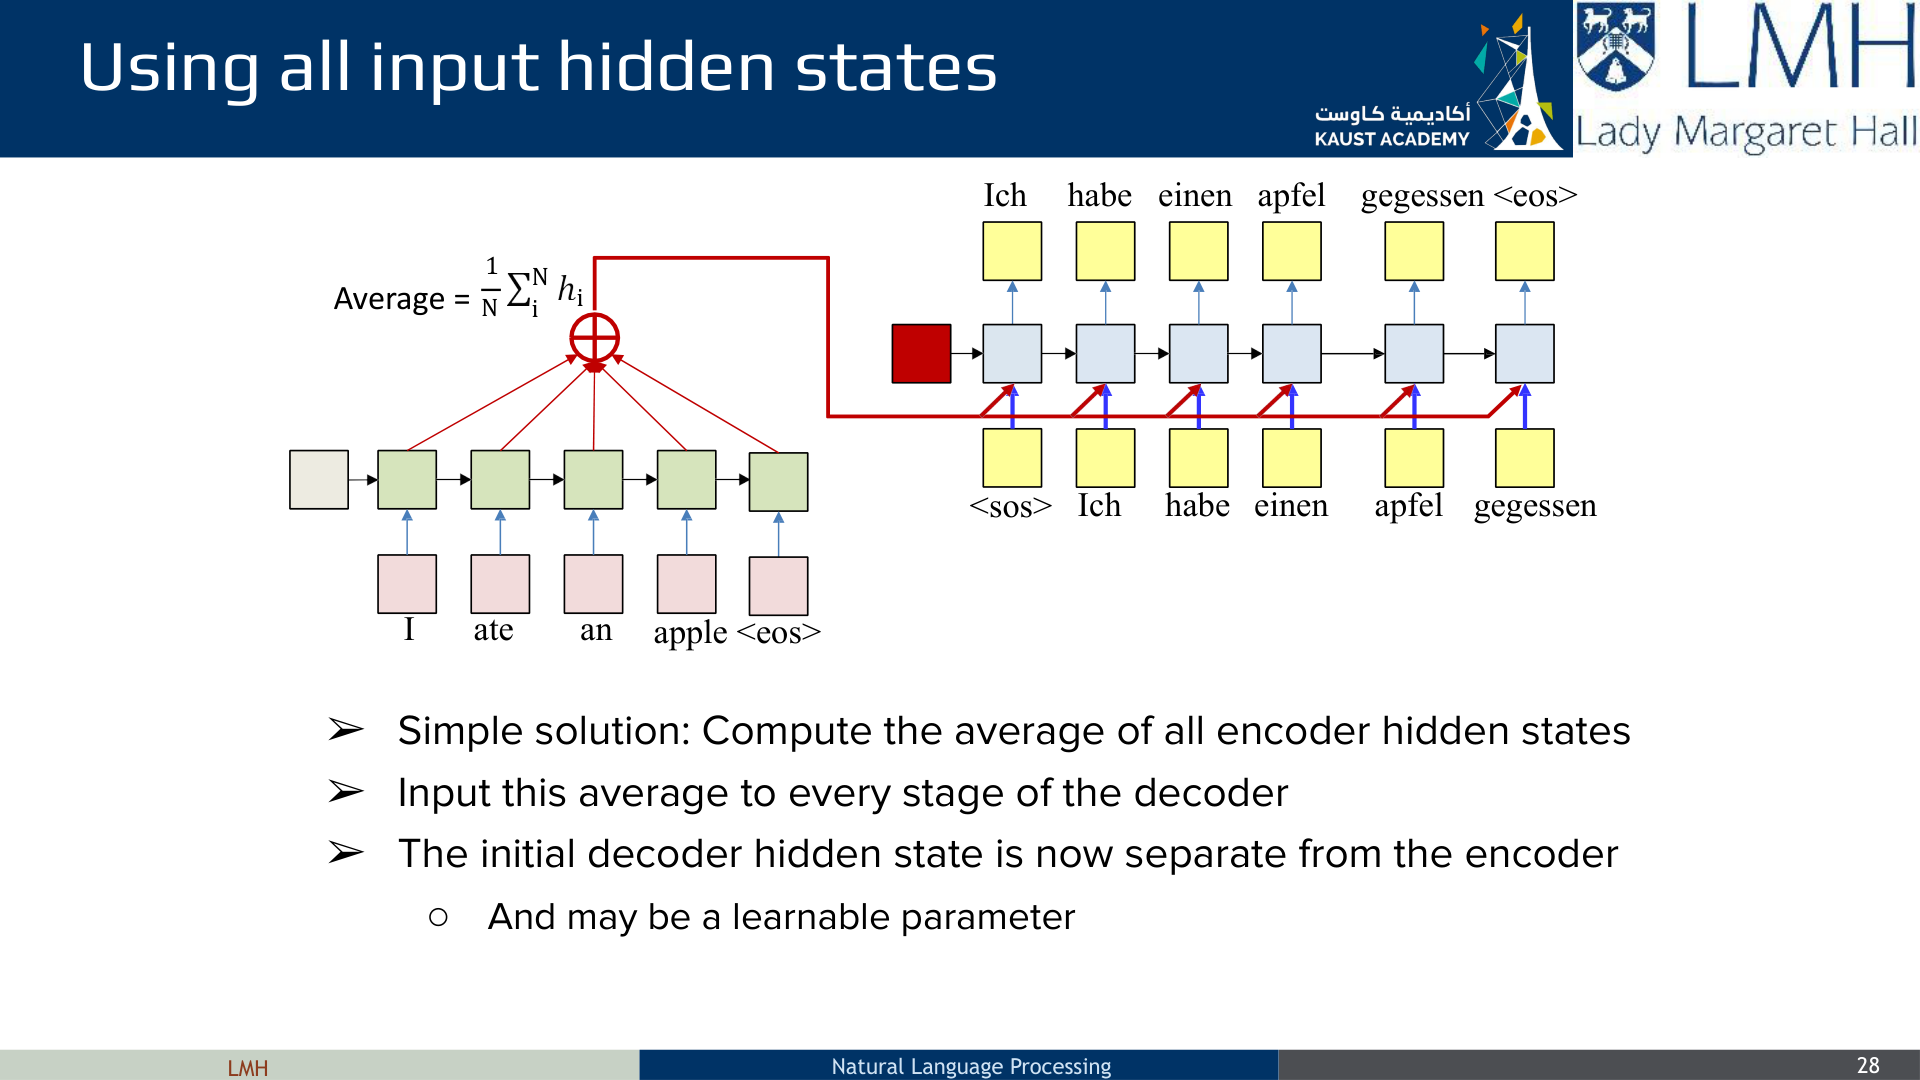
\includegraphics[width=\paperwidth,height=0.95\paperheight,keepaspectratio]{assets/Lecture-11_Large_Reasoning_Models_and_Mixture_of_Experts_Models/pdf_page_028.png}
\end{frame}

\begin{frame}[plain]
  \centering
  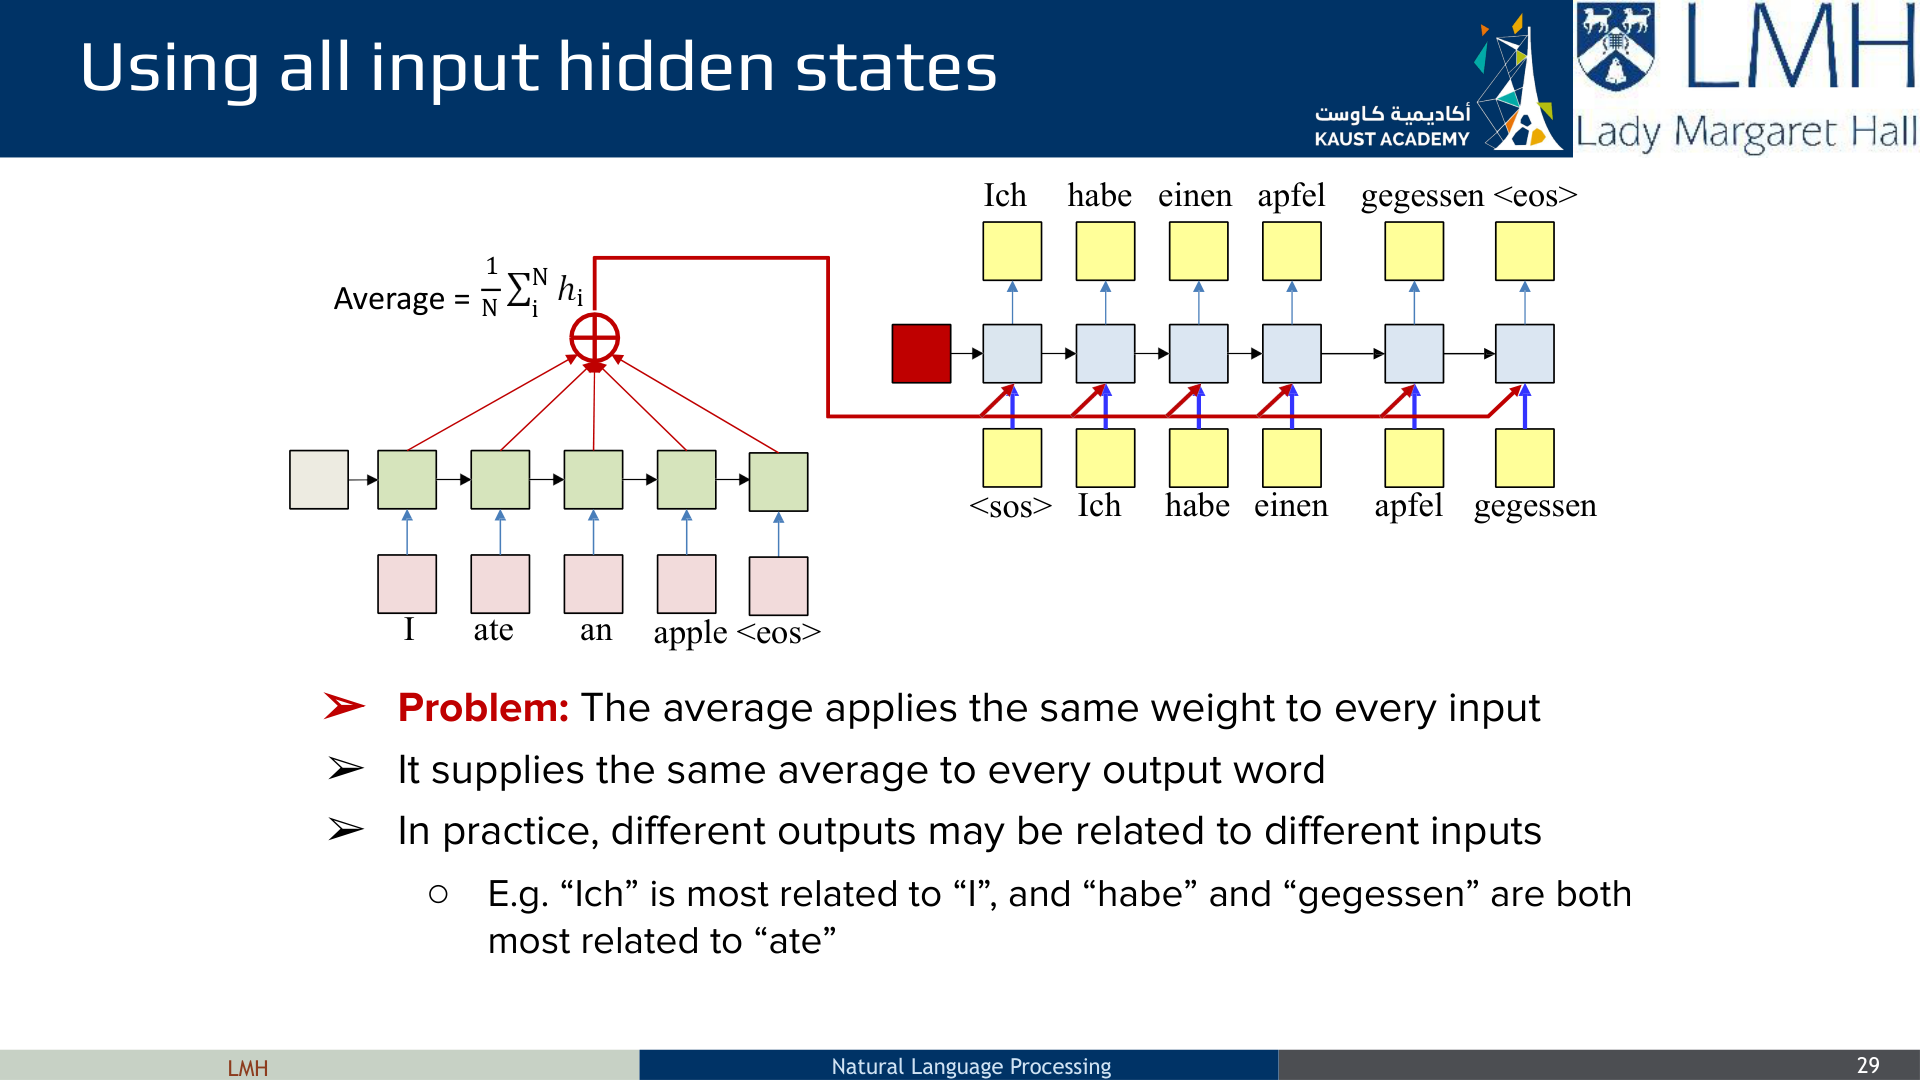
\includegraphics[width=\paperwidth,height=0.95\paperheight,keepaspectratio]{assets/Lecture-11_Large_Reasoning_Models_and_Mixture_of_Experts_Models/pdf_page_029.png}
\end{frame}

\begin{frame}[plain]
  \centering
  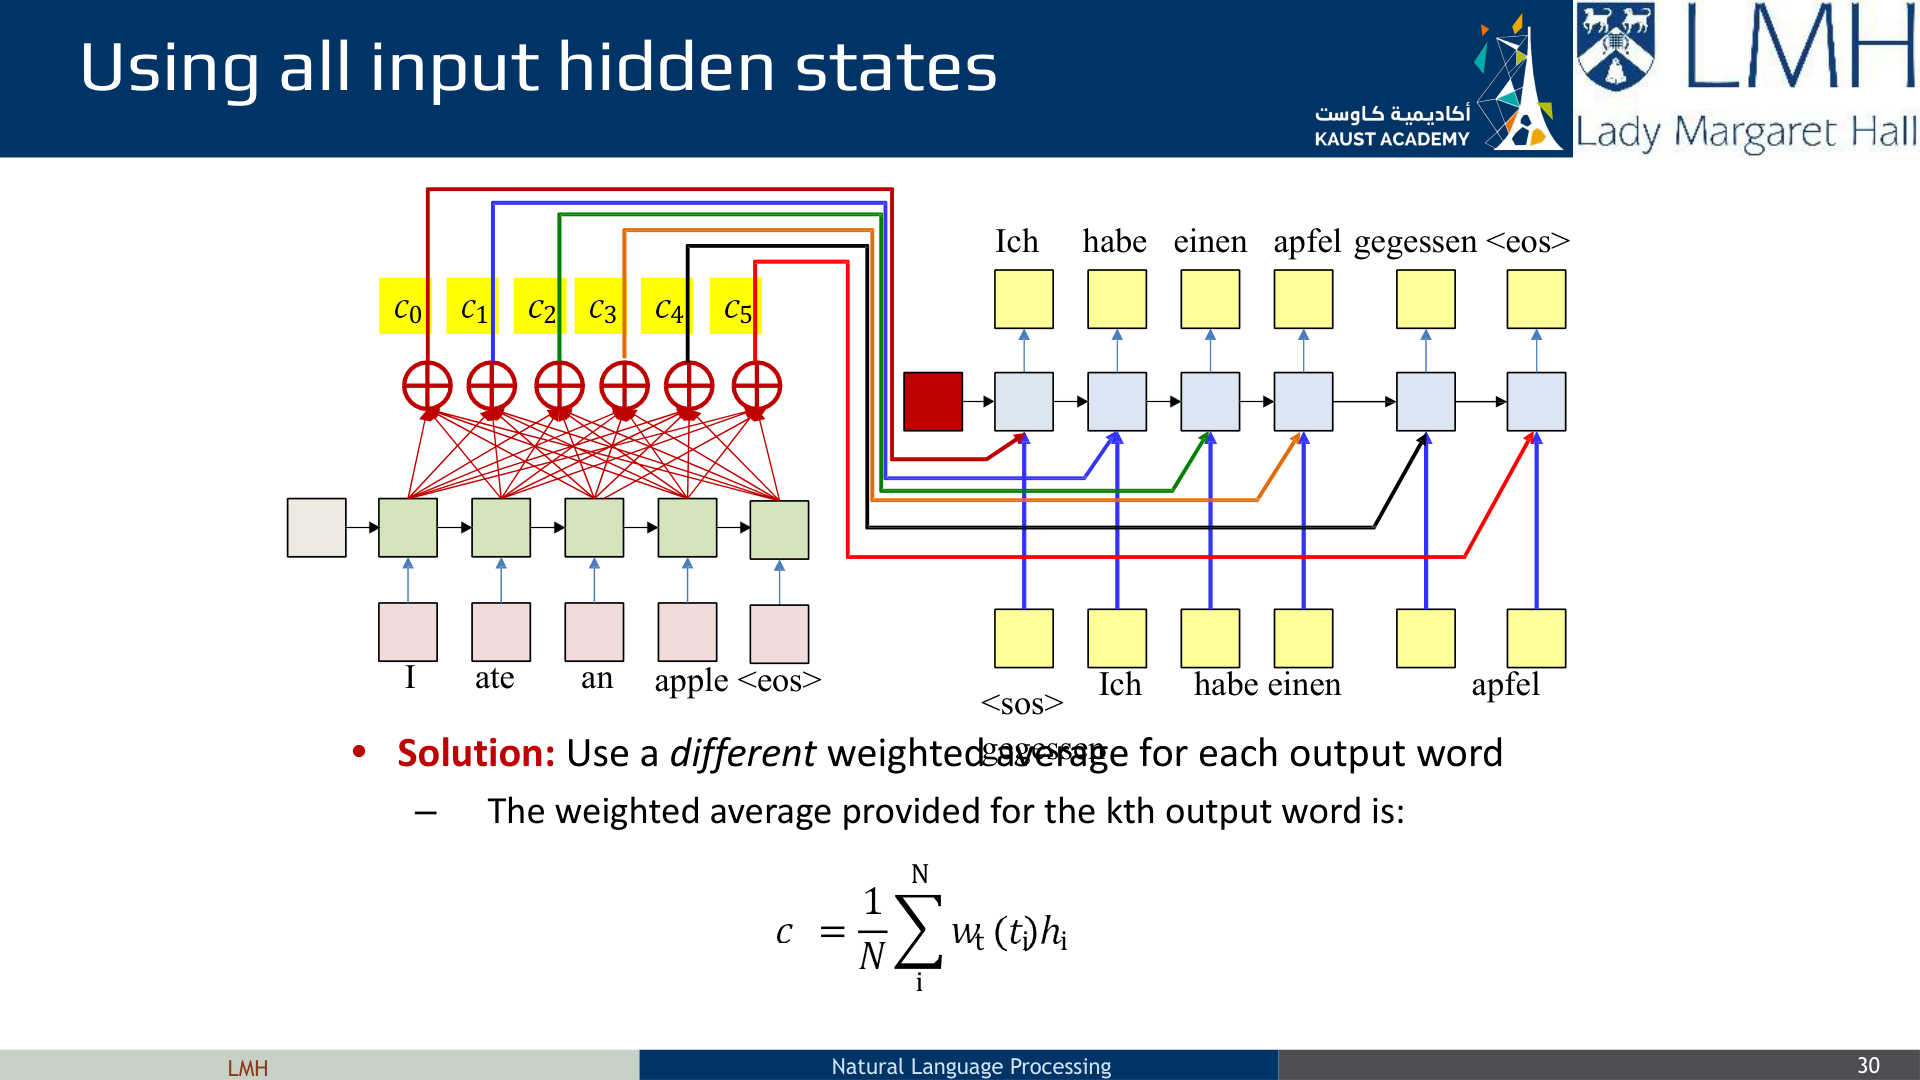
\includegraphics[width=\paperwidth,height=0.95\paperheight,keepaspectratio]{assets/Lecture-11_Large_Reasoning_Models_and_Mixture_of_Experts_Models/pdf_page_030.png}
\end{frame}

\begin{frame}[plain]
  \centering
  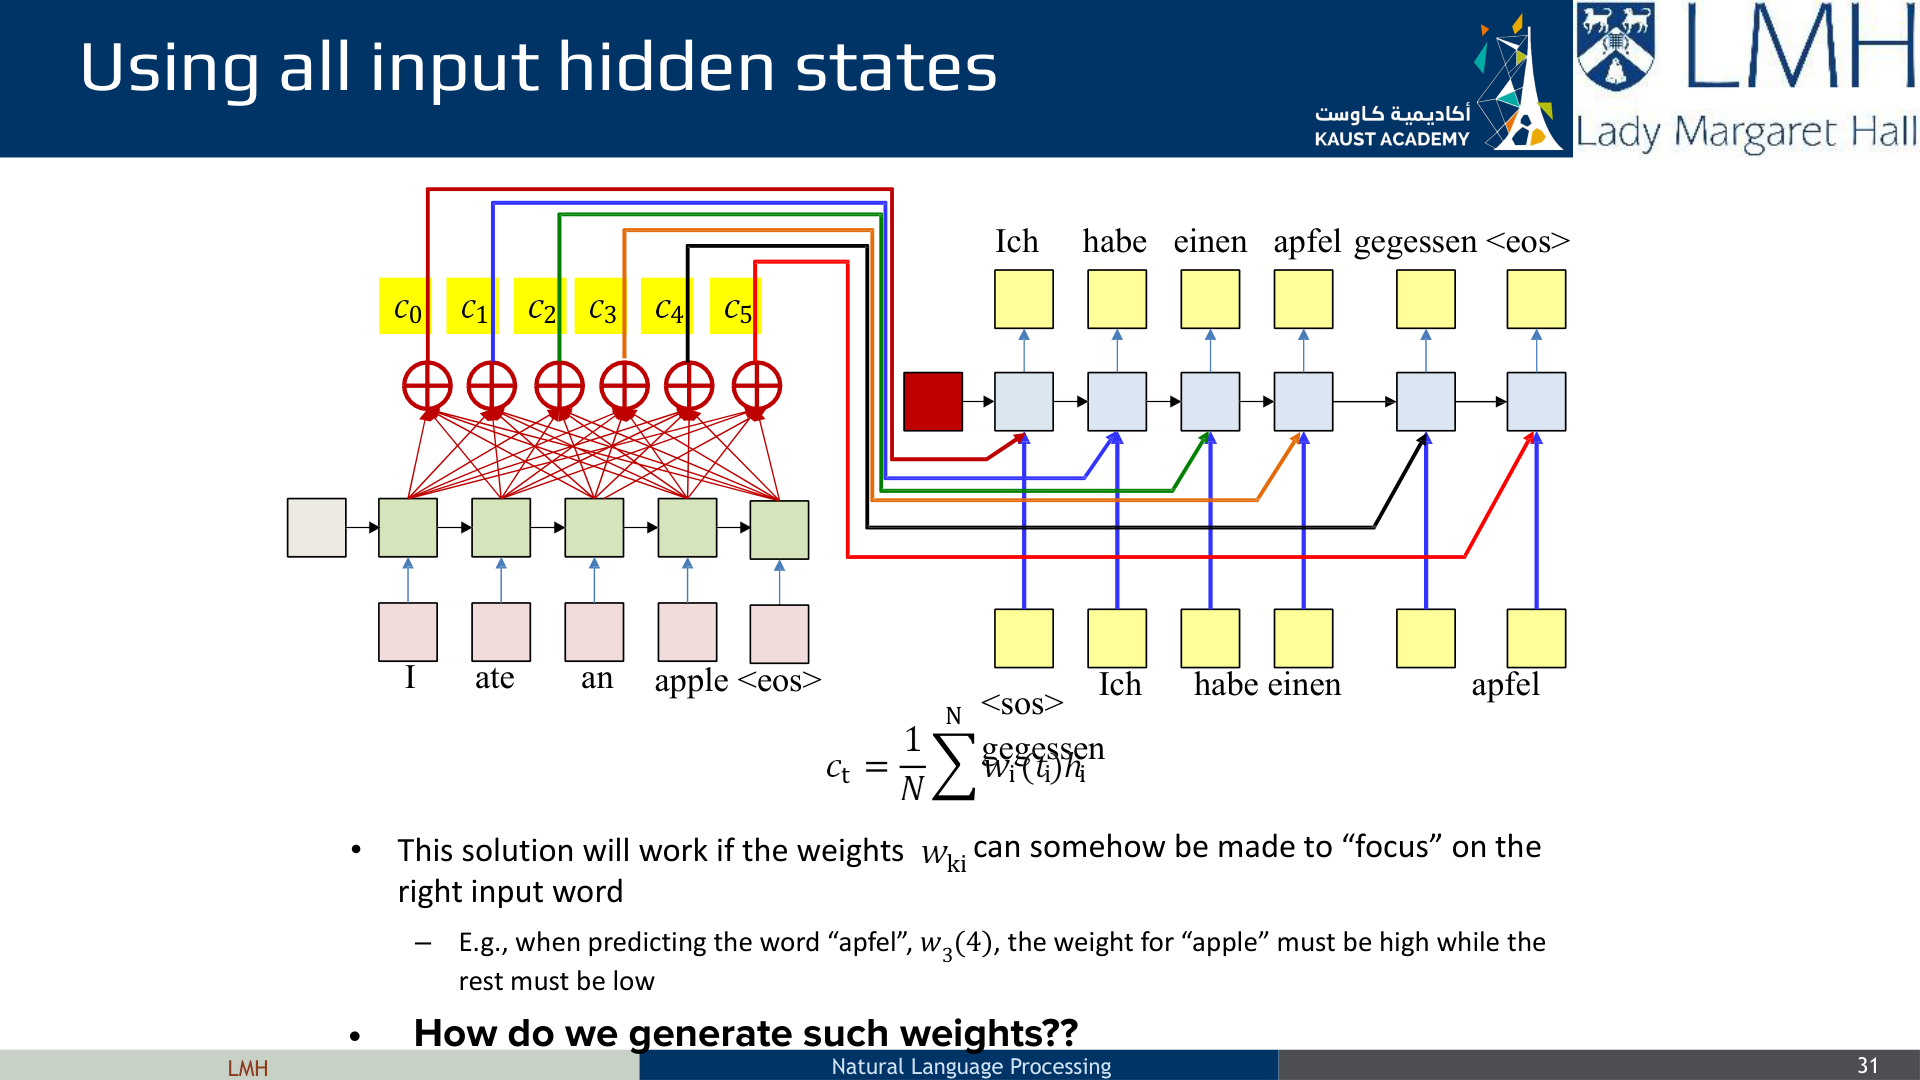
\includegraphics[width=\paperwidth,height=0.95\paperheight,keepaspectratio]{assets/Lecture-11_Large_Reasoning_Models_and_Mixture_of_Experts_Models/pdf_page_031.png}
\end{frame}

\begin{frame}[t]{Natural Language Processing}
  \begin{itemize}
    \item LMH
    \item 32
    \item Introduction to Attention Mechanism
  \end{itemize}
\end{frame}

\begin{frame}[plain]
  \centering
  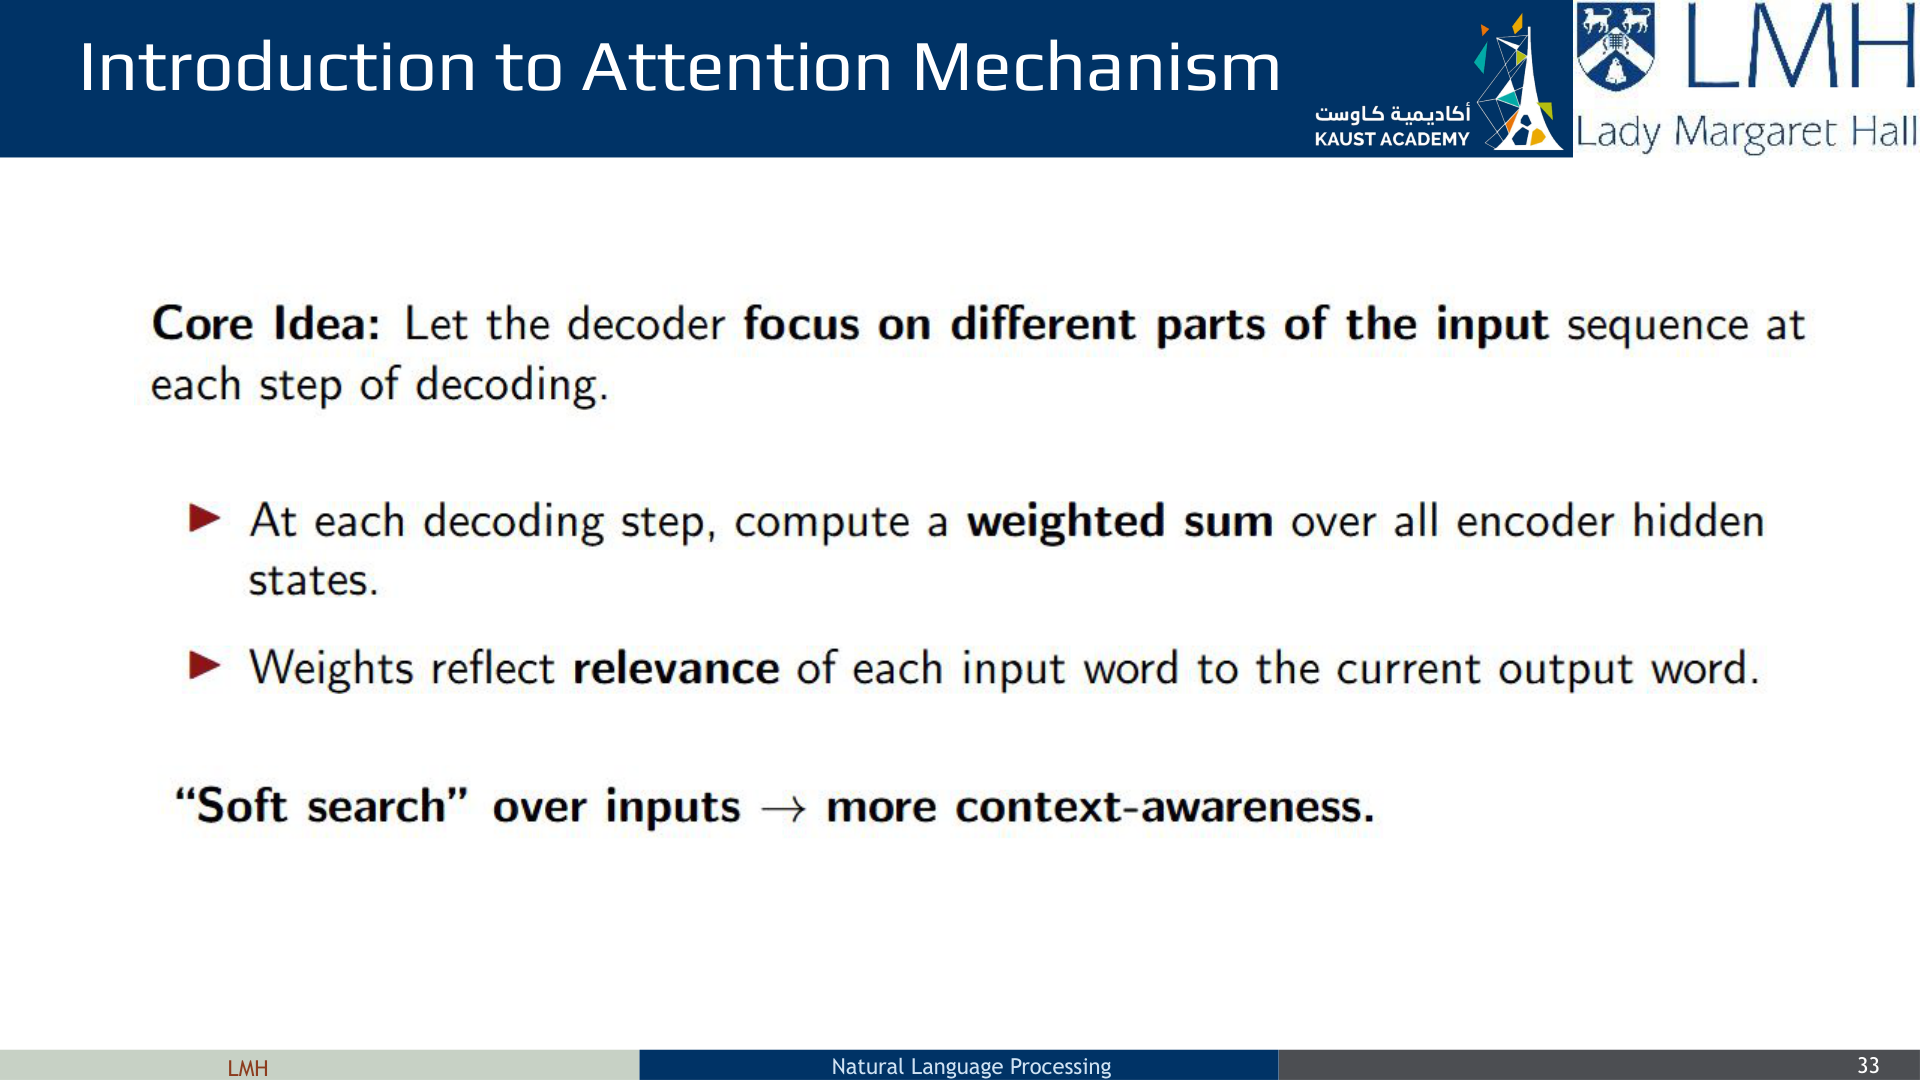
\includegraphics[width=\paperwidth,height=0.95\paperheight,keepaspectratio]{assets/Lecture-11_Large_Reasoning_Models_and_Mixture_of_Experts_Models/pdf_page_033.png}
\end{frame}

\begin{frame}[t]{Natural Language Processing}
  \begin{itemize}
    \item LMH
    \item 34
    \item Mathematical Formulation of Attention
  \end{itemize}
\end{frame}

\begin{frame}[plain]
  \centering
  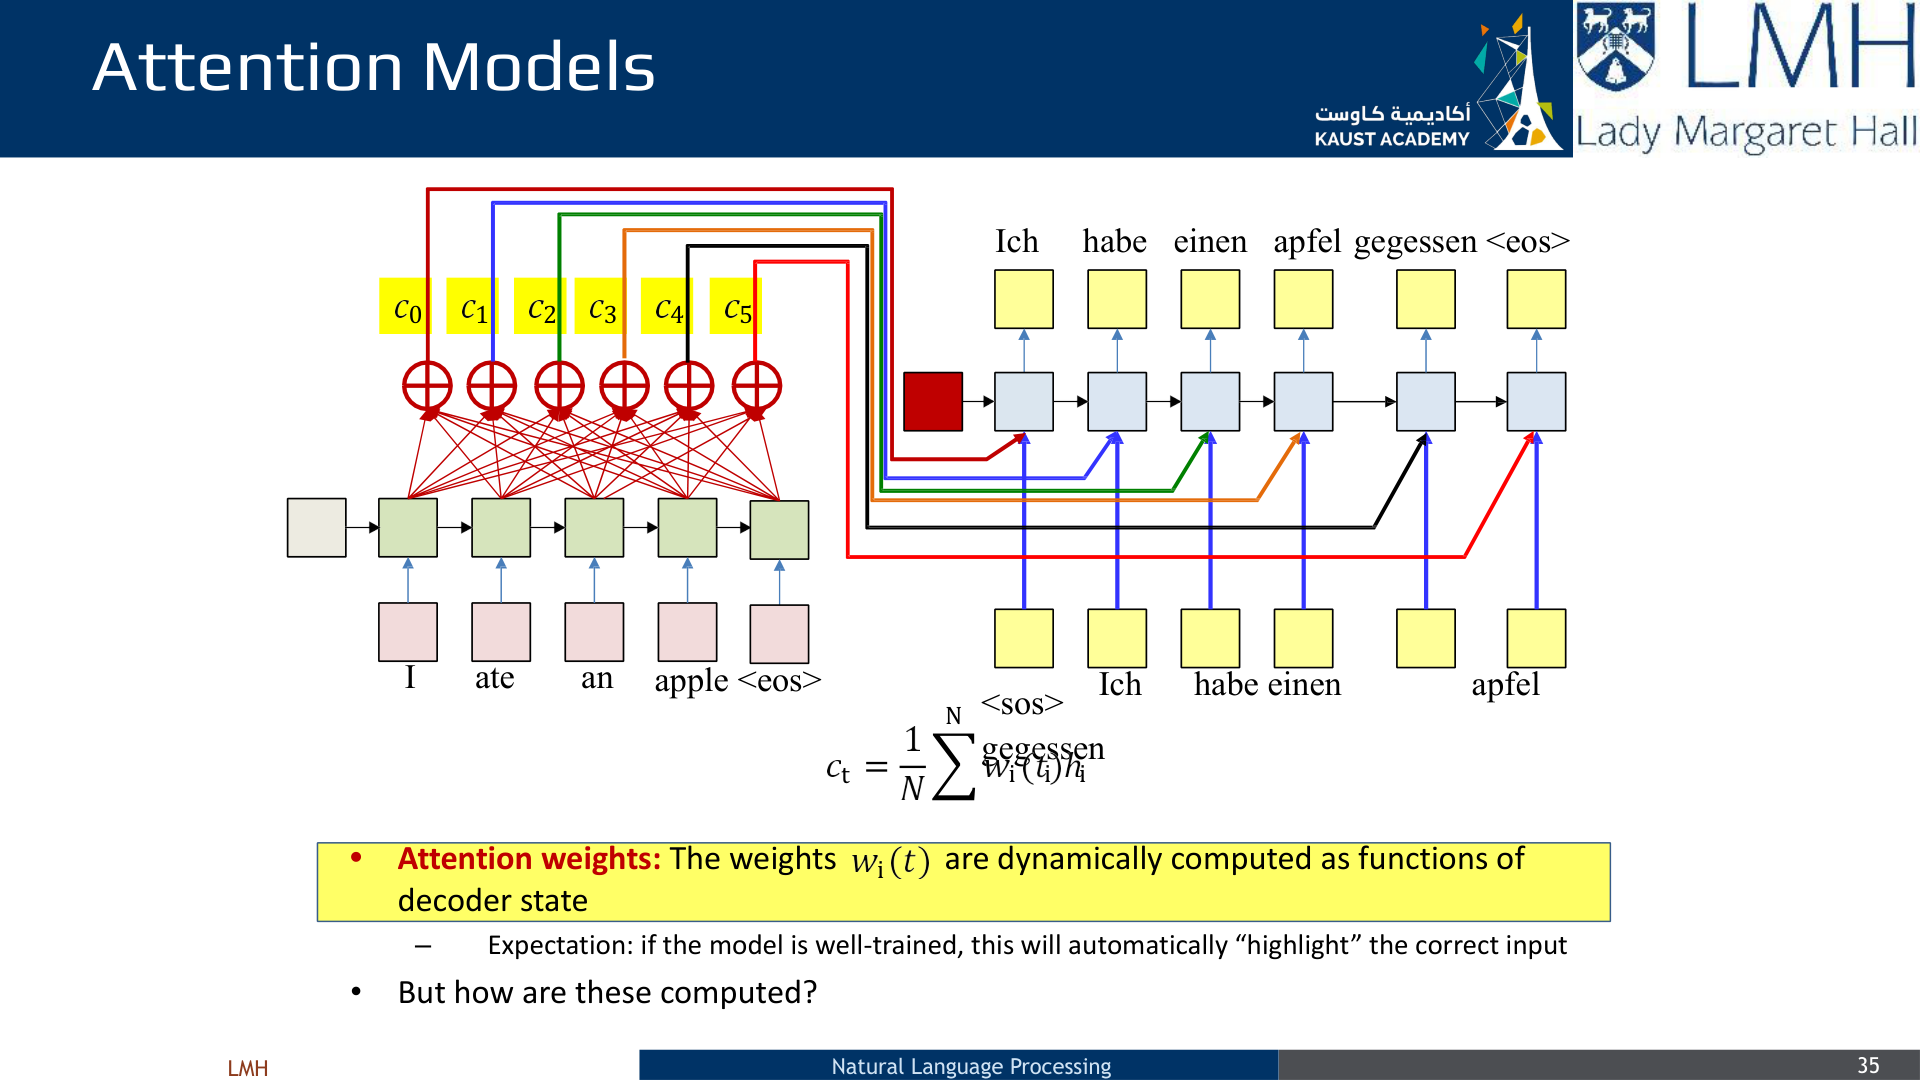
\includegraphics[width=\paperwidth,height=0.95\paperheight,keepaspectratio]{assets/Lecture-11_Large_Reasoning_Models_and_Mixture_of_Experts_Models/pdf_page_035.png}
\end{frame}

\begin{frame}[plain]
  \centering
  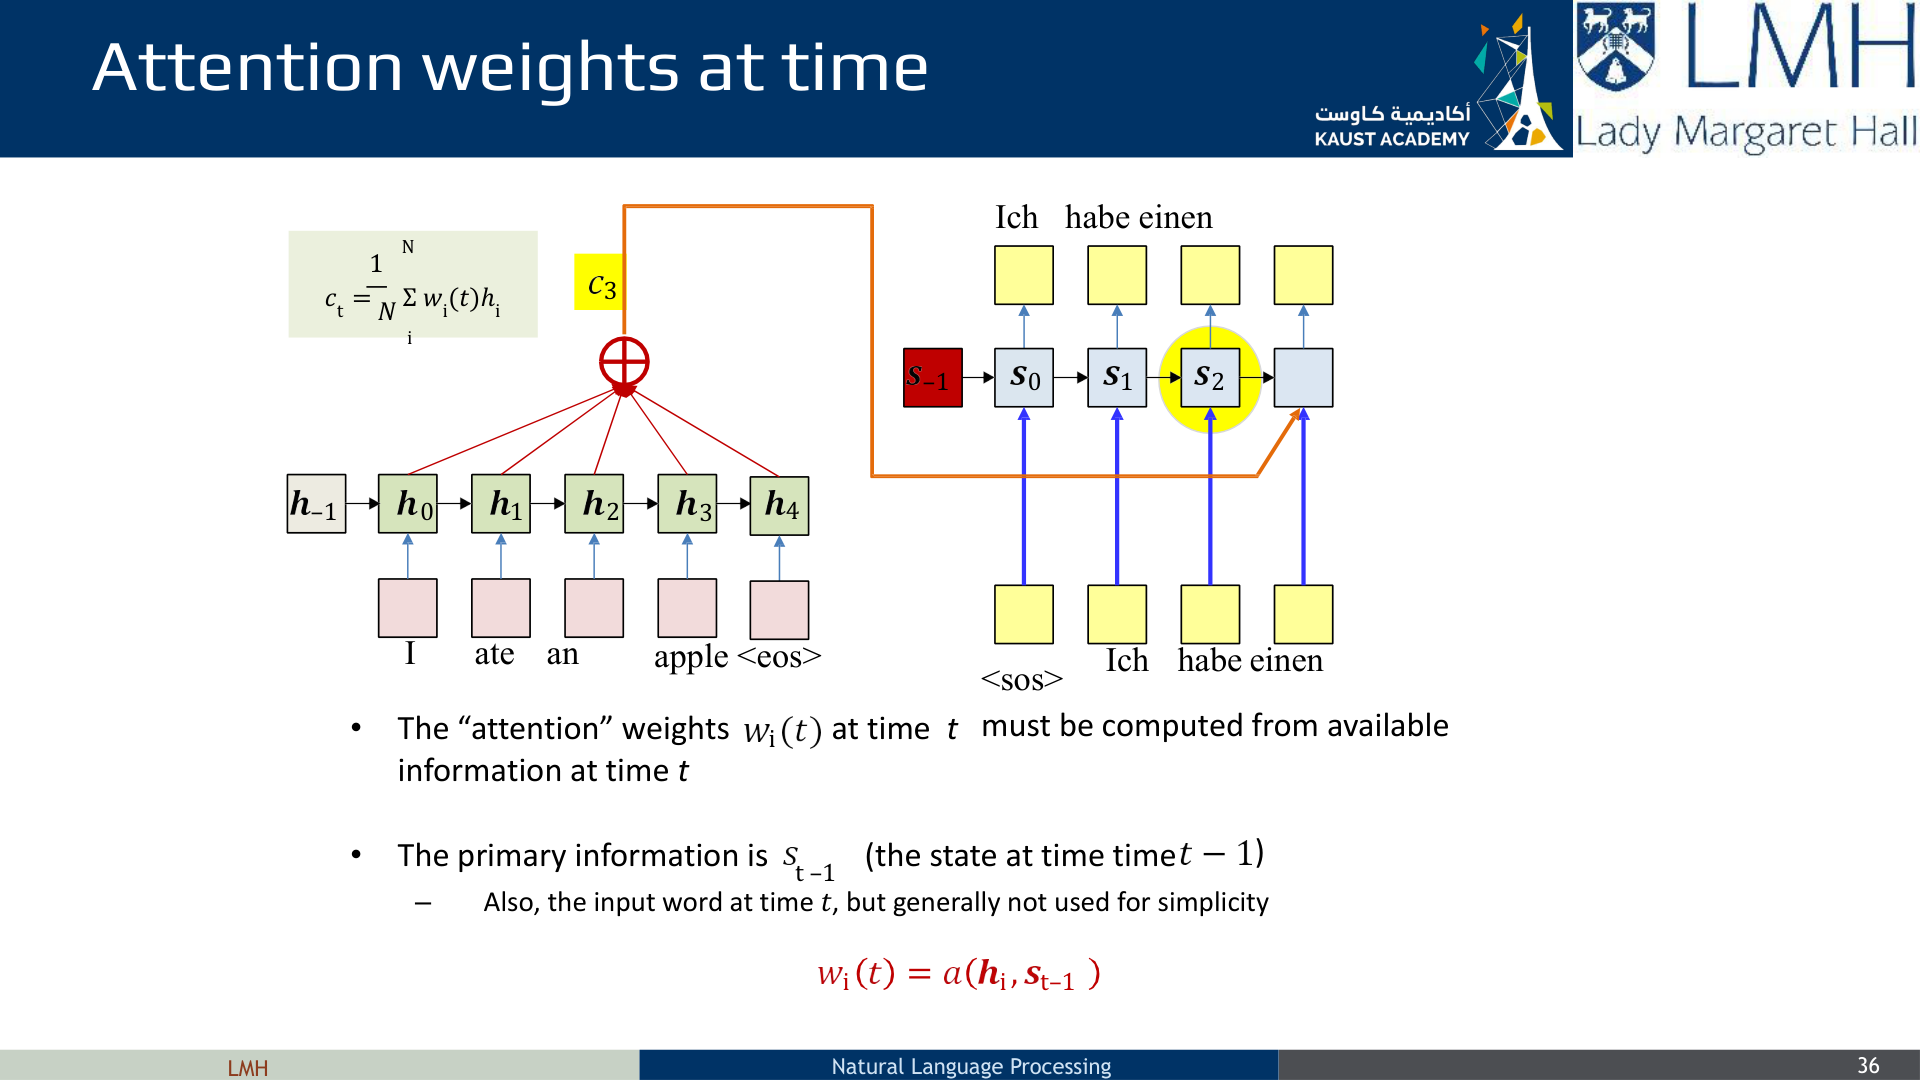
\includegraphics[width=\paperwidth,height=0.95\paperheight,keepaspectratio]{assets/Lecture-11_Large_Reasoning_Models_and_Mixture_of_Experts_Models/pdf_page_036.png}
\end{frame}

\begin{frame}[plain]
  \centering
  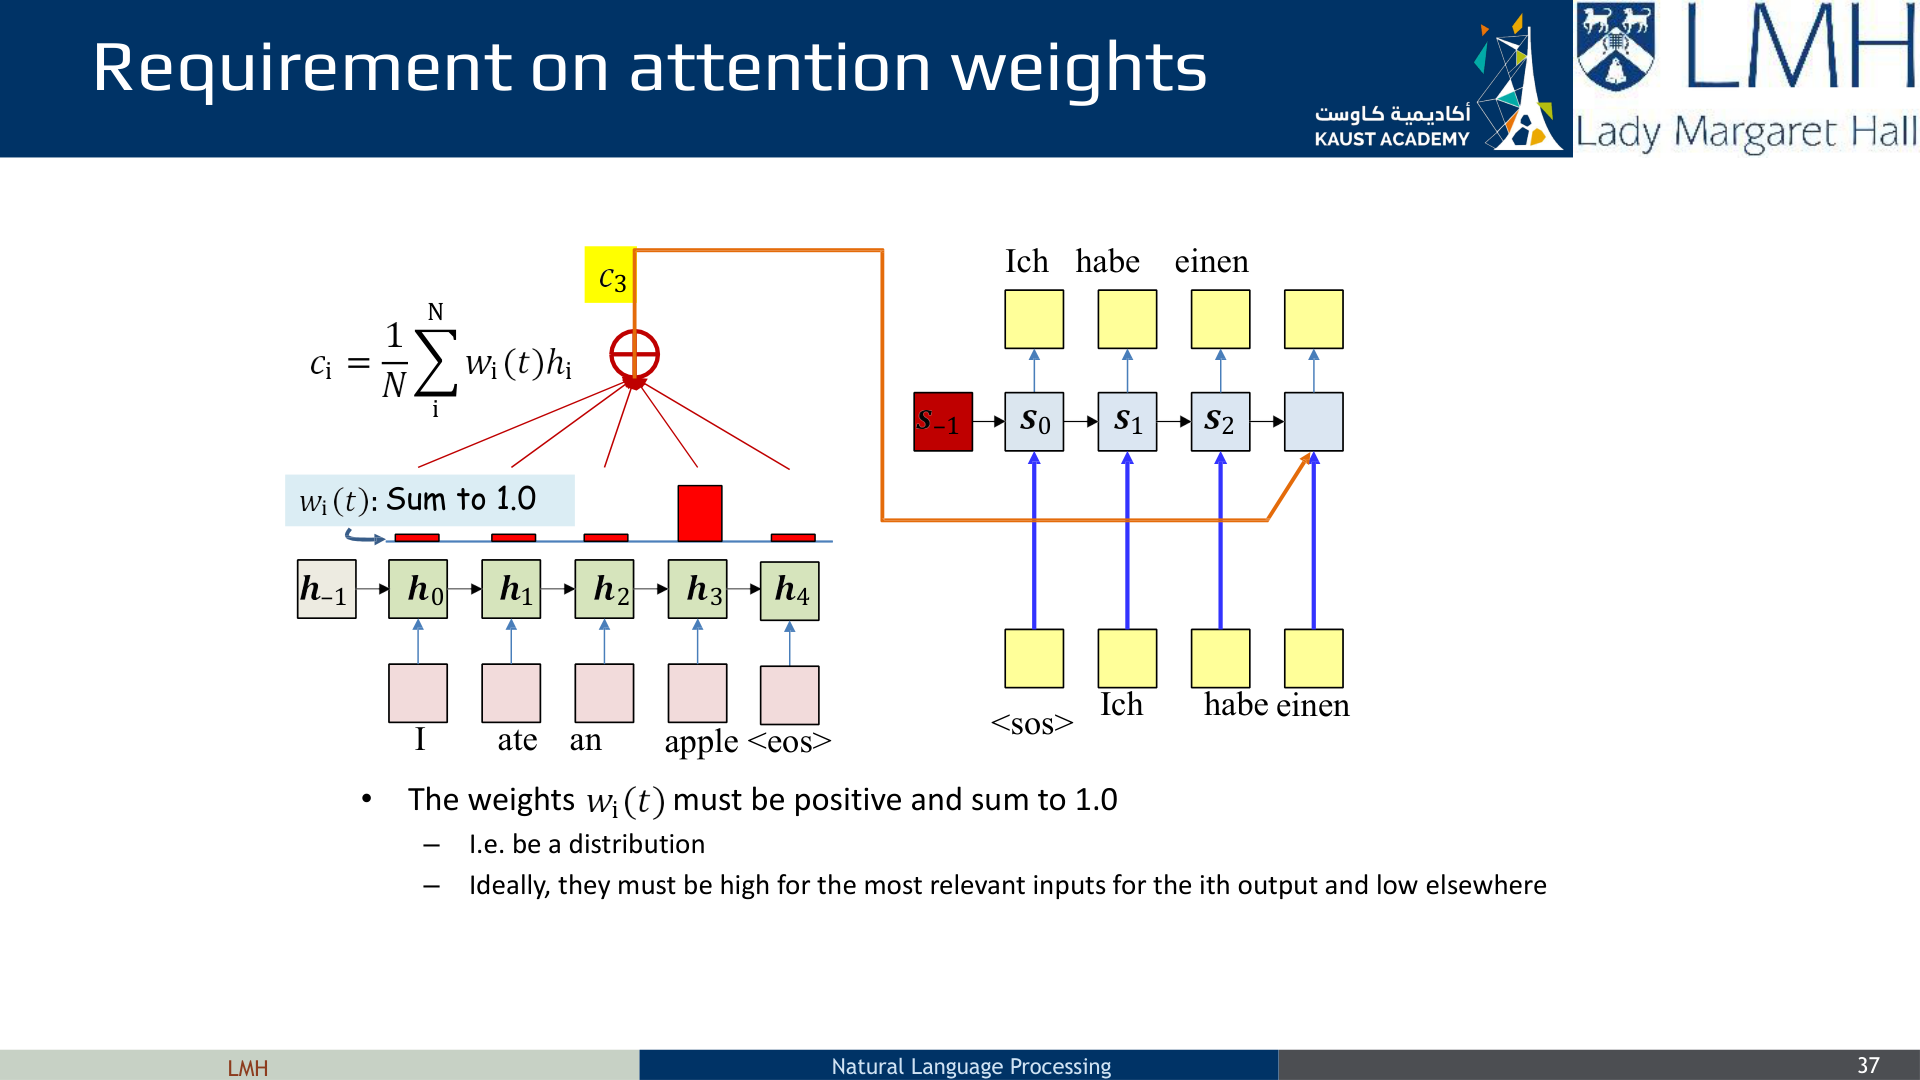
\includegraphics[width=\paperwidth,height=0.95\paperheight,keepaspectratio]{assets/Lecture-11_Large_Reasoning_Models_and_Mixture_of_Experts_Models/pdf_page_037.png}
\end{frame}

\begin{frame}[plain]
  \centering
  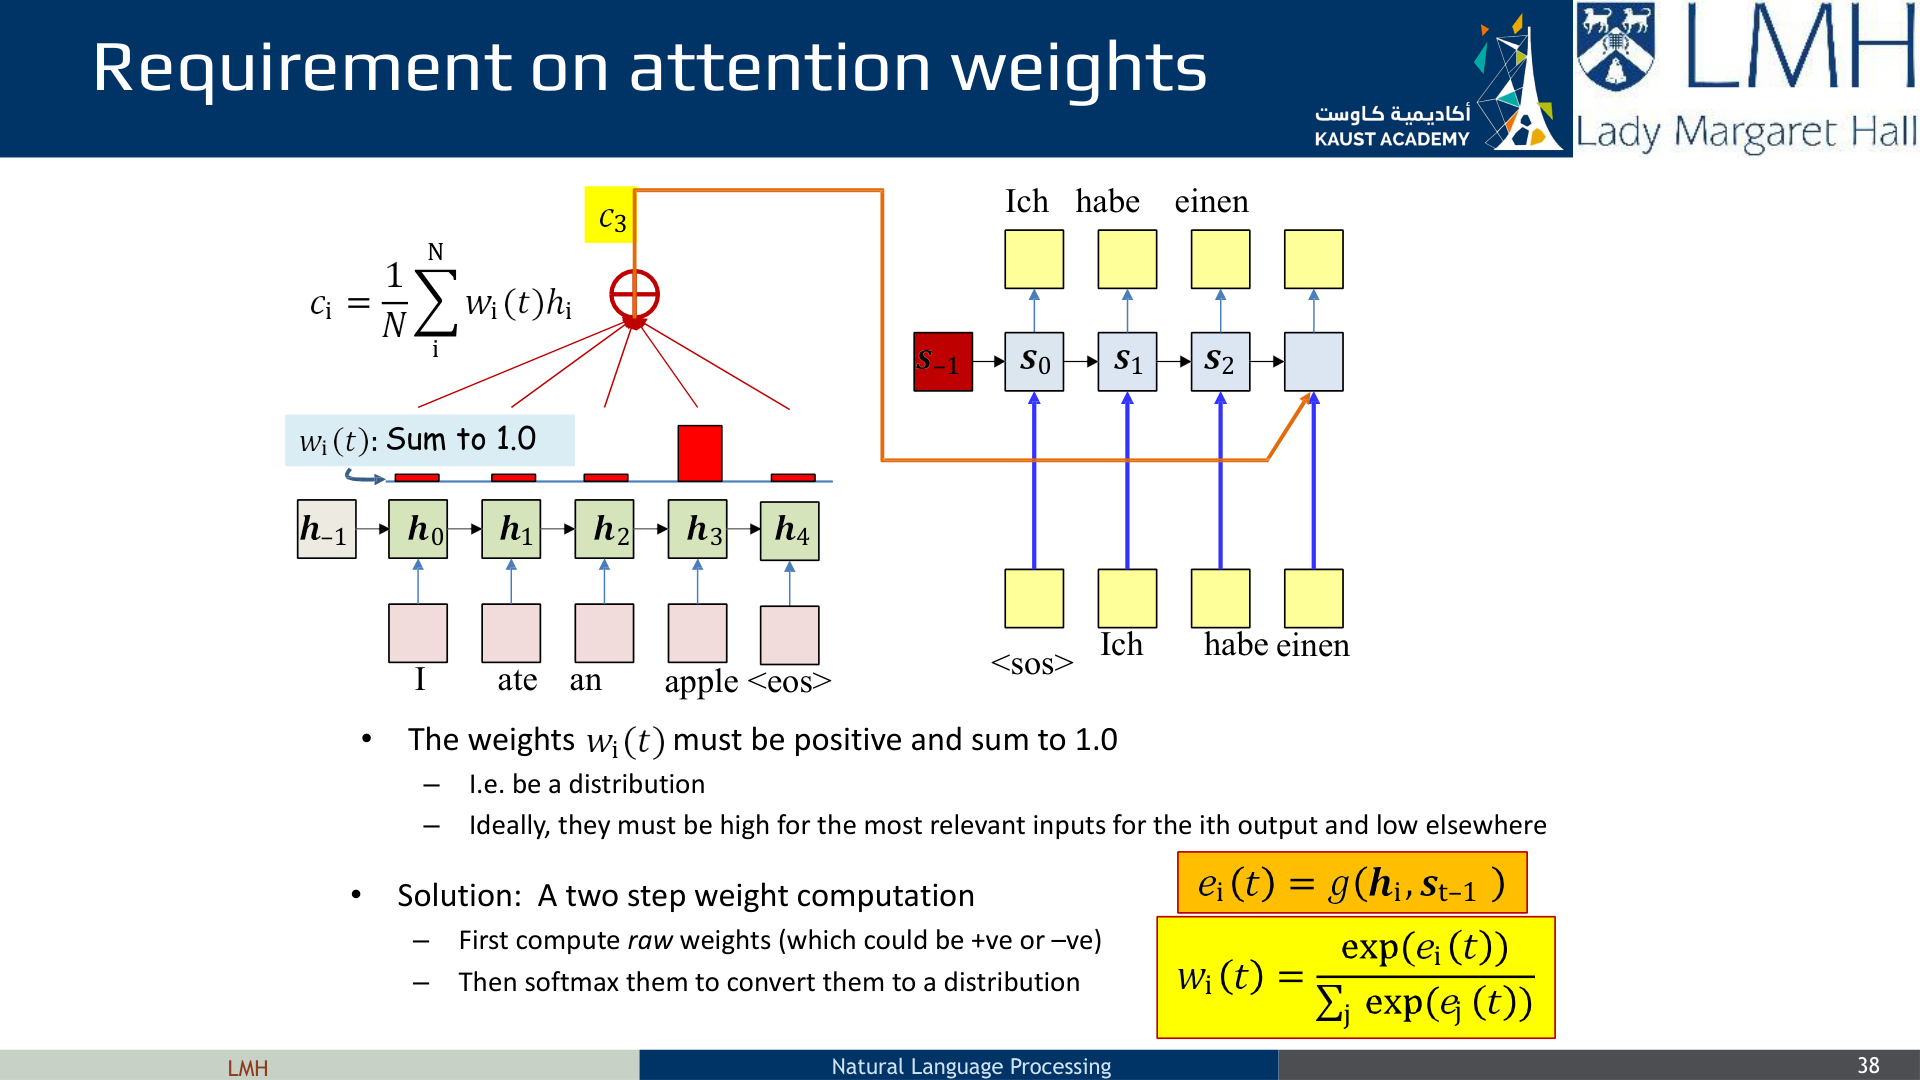
\includegraphics[width=\paperwidth,height=0.95\paperheight,keepaspectratio]{assets/Lecture-11_Large_Reasoning_Models_and_Mixture_of_Experts_Models/pdf_page_038.png}
\end{frame}

\begin{frame}[t]{Natural Language Processing}
  \begin{itemize}
    \item LMH
    \item 39
    \item Quiz
    \item 1.
    \item The attention framework computes a different "context" vector at each output step (T/F)
    \item a.
    \item True
    \item b.
    \item False
    \item 2.
    \item The context vector is chosen as the hidden (encoder) representation of the input word that
    \item is assigned the highest attention weight (T/F)
    \item a.
    \item True
    \item b.
    \item False
    \item 3.
    \item The attention weight to any input word is a function of the hidden encoder representation of
    \item the word and the most recent decoder state (T/F)
    \item a.
    \item True
    \item b.
    \item False
  \end{itemize}
\end{frame}

\begin{frame}[t]{Natural Language Processing}
  \begin{itemize}
    \item LMH
    \item 40
    \item Quiz: Answer
    \item 1.
    \item The attention framework computes a different "context" vector at each output step (T/F)
    \item a.
    \item True
    \item b.
    \item False
    \item 2.
    \item The context vector is chosen as the hidden (encoder) representation of the input word that
    \item is assigned the highest attention weight (T/F)
    \item a.
    \item True
    \item b.
    \item False
    \item 3.
    \item The attention weight to any input word is a function of the hidden encoder representation of
    \item the word and the most recent decoder state (T/F)
    \item a.
    \item True
    \item b.
    \item False
  \end{itemize}
\end{frame}

\begin{frame}[plain]
  \centering
  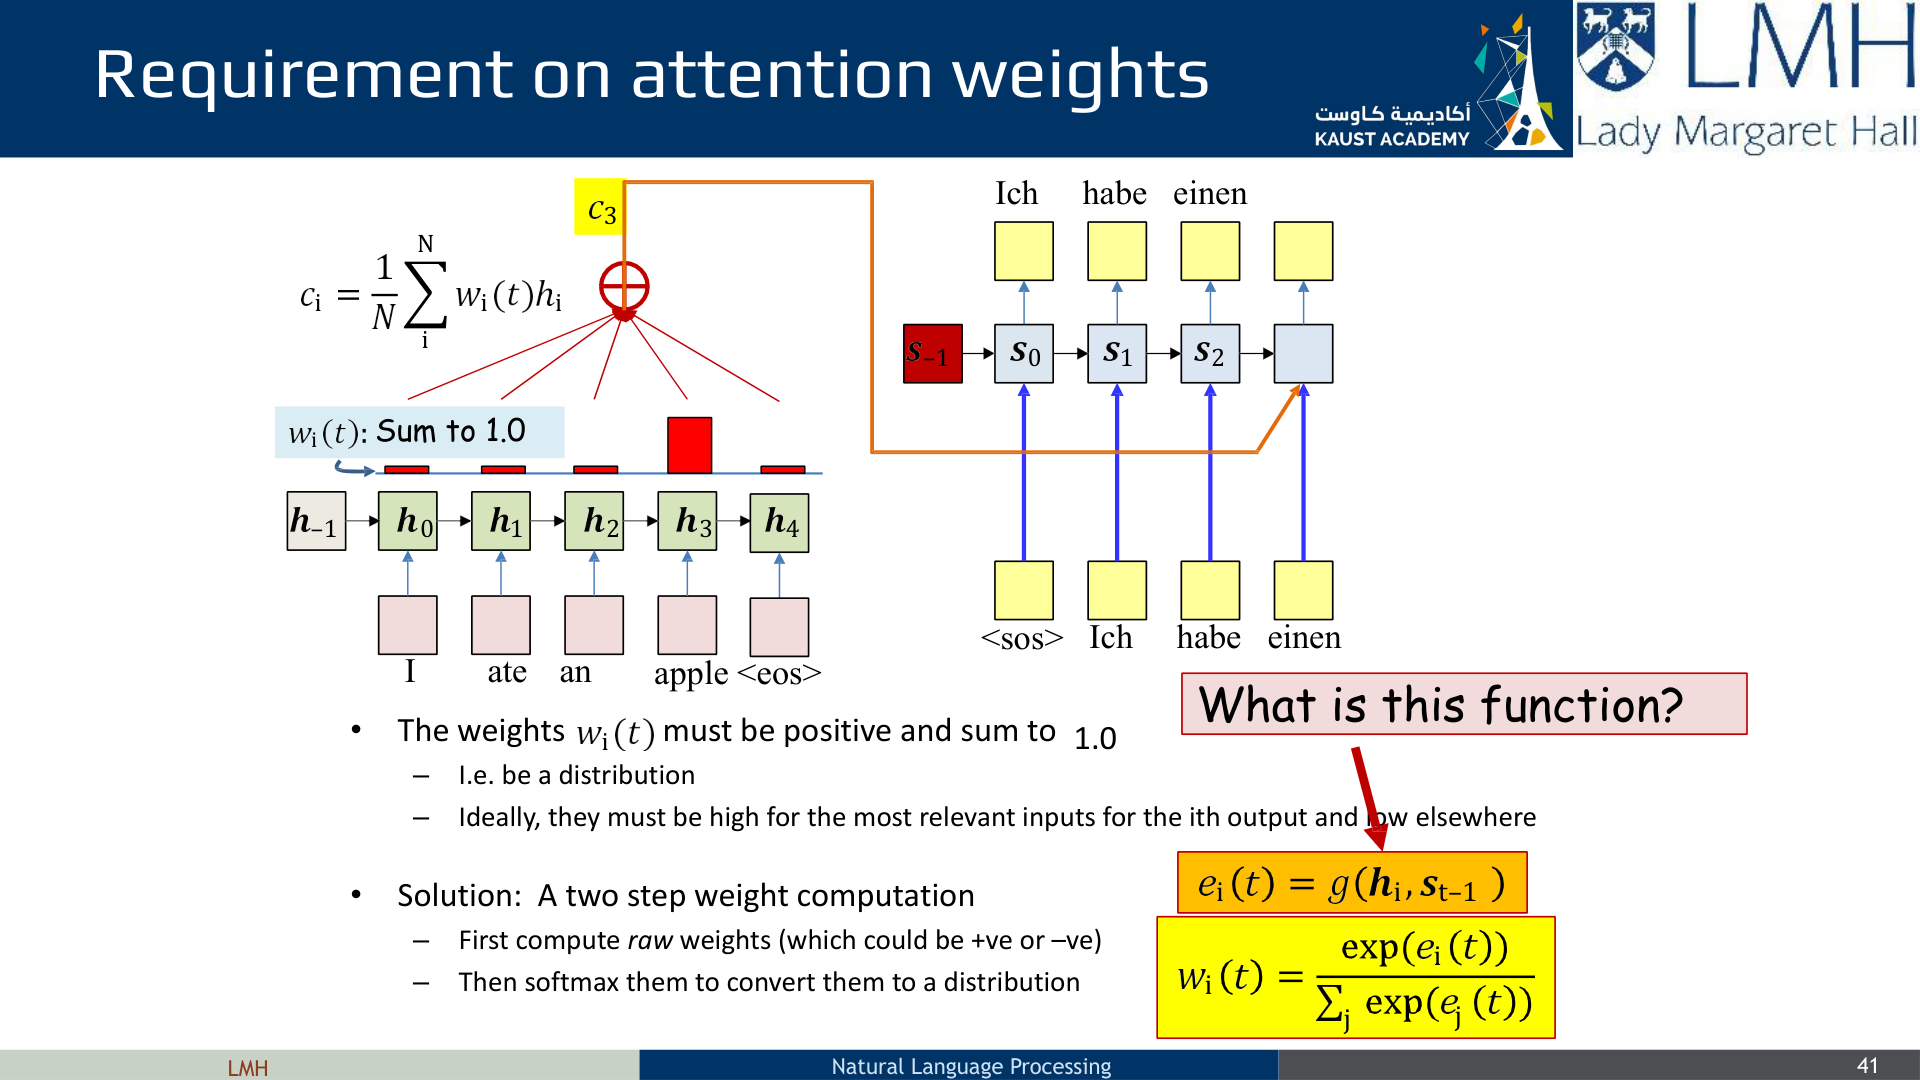
\includegraphics[width=\paperwidth,height=0.95\paperheight,keepaspectratio]{assets/Lecture-11_Large_Reasoning_Models_and_Mixture_of_Experts_Models/pdf_page_041.png}
\end{frame}

\begin{frame}[plain]
  \centering
  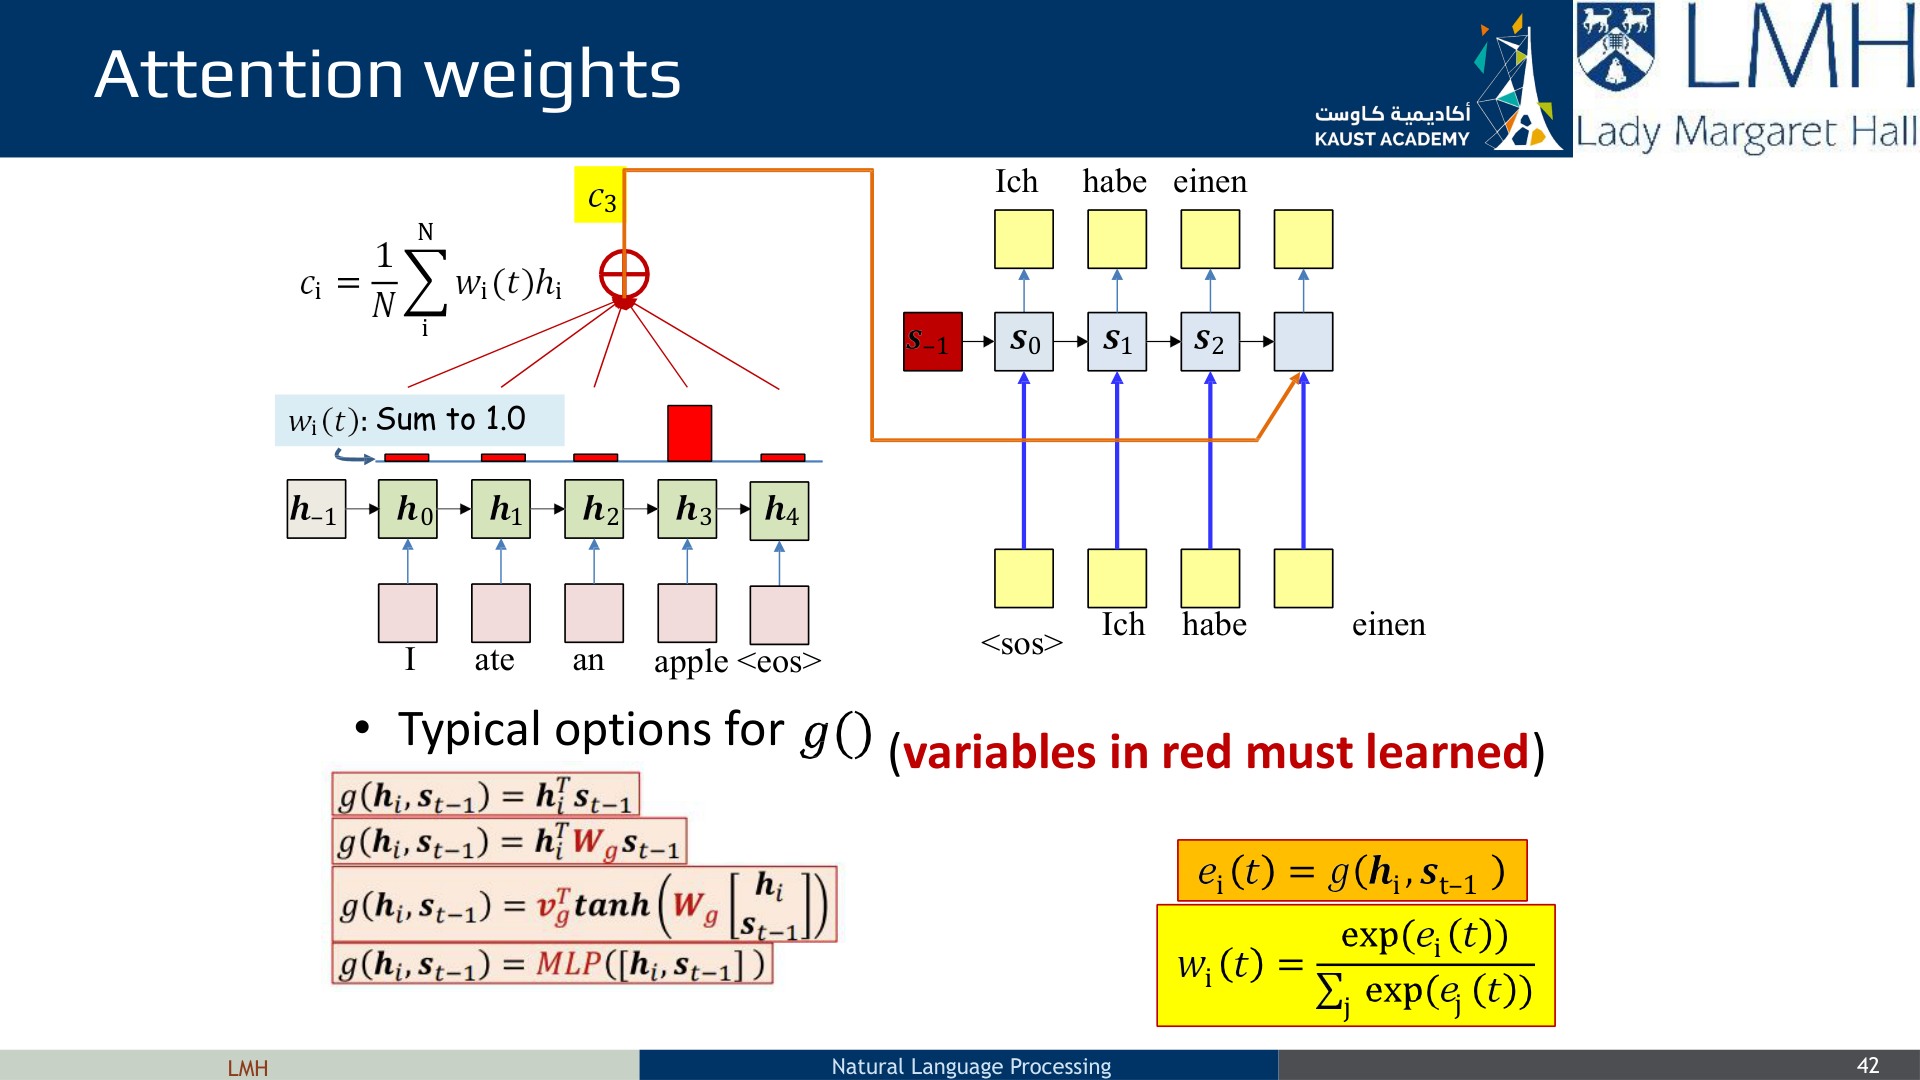
\includegraphics[width=\paperwidth,height=0.95\paperheight,keepaspectratio]{assets/Lecture-11_Large_Reasoning_Models_and_Mixture_of_Experts_Models/pdf_page_042.png}
\end{frame}

\begin{frame}[plain]
  \centering
  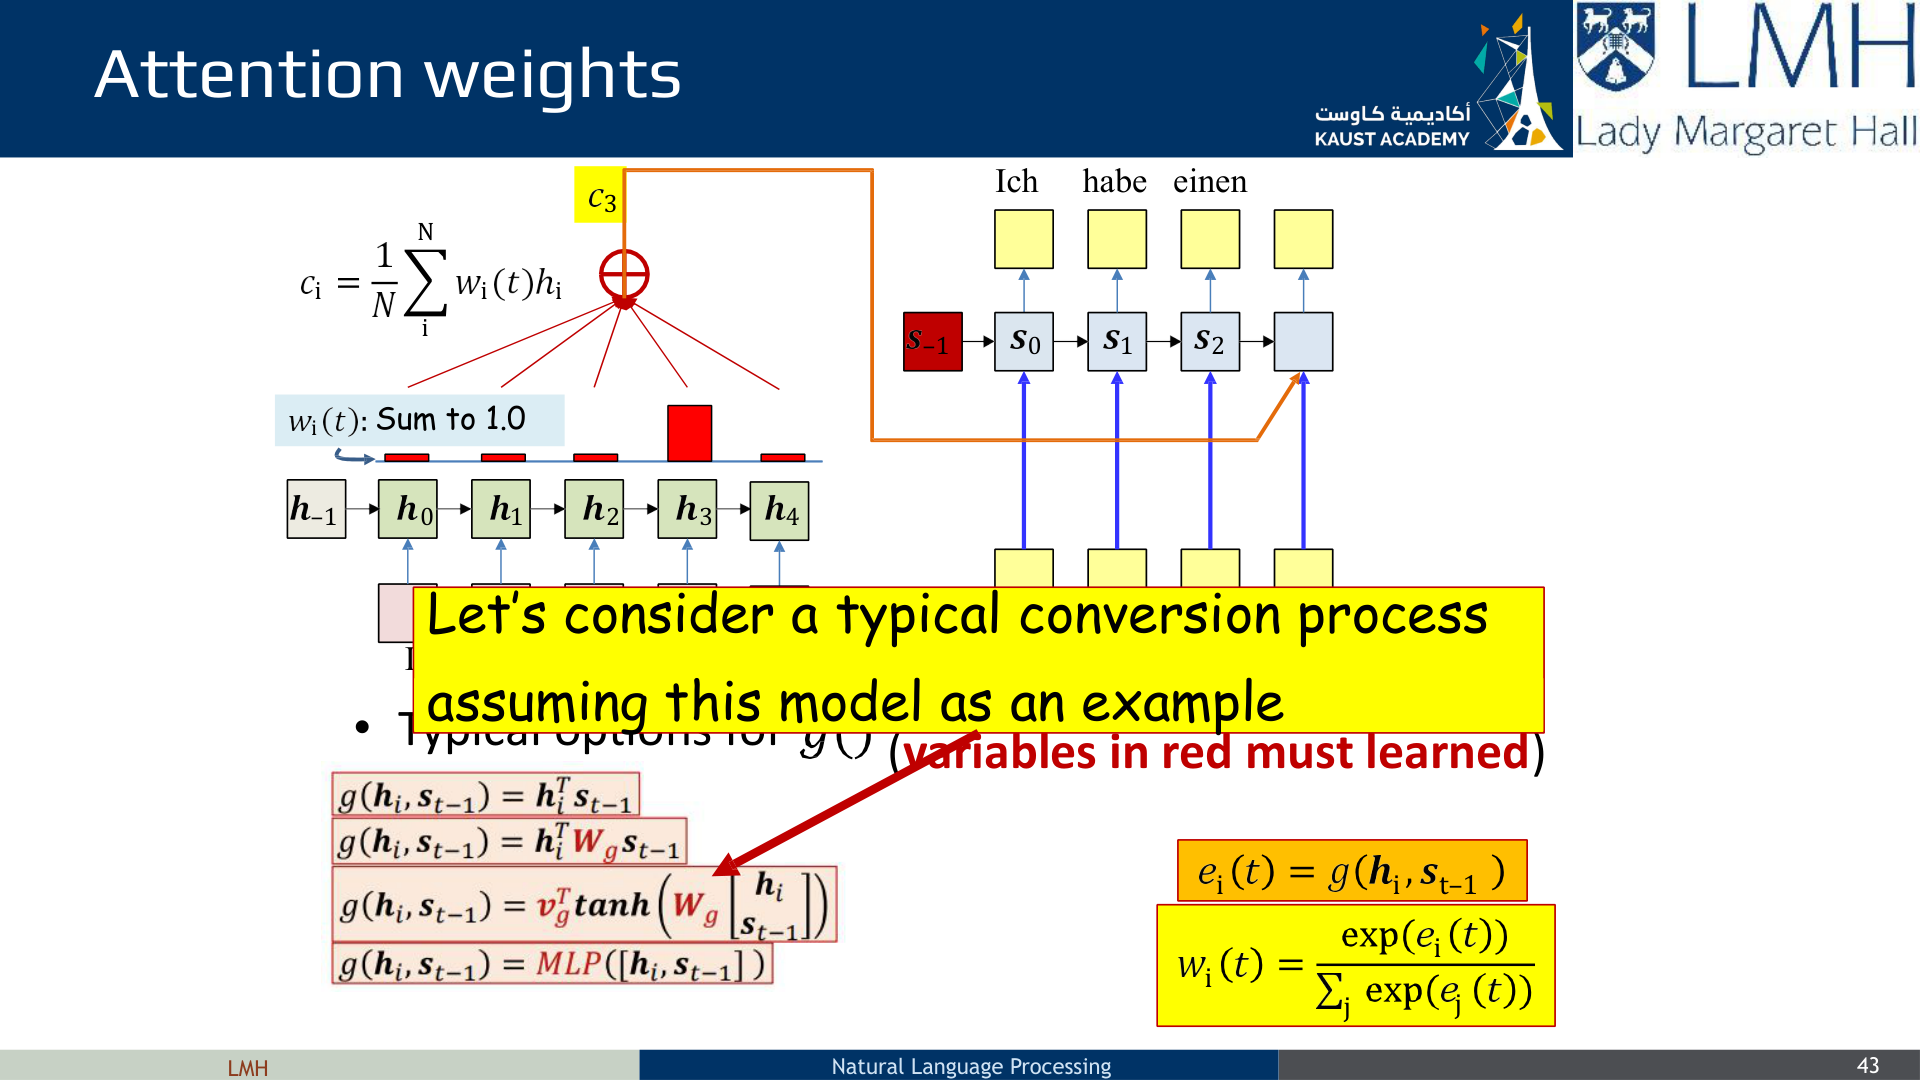
\includegraphics[width=\paperwidth,height=0.95\paperheight,keepaspectratio]{assets/Lecture-11_Large_Reasoning_Models_and_Mixture_of_Experts_Models/pdf_page_043.png}
\end{frame}

\begin{frame}[plain]
  \centering
  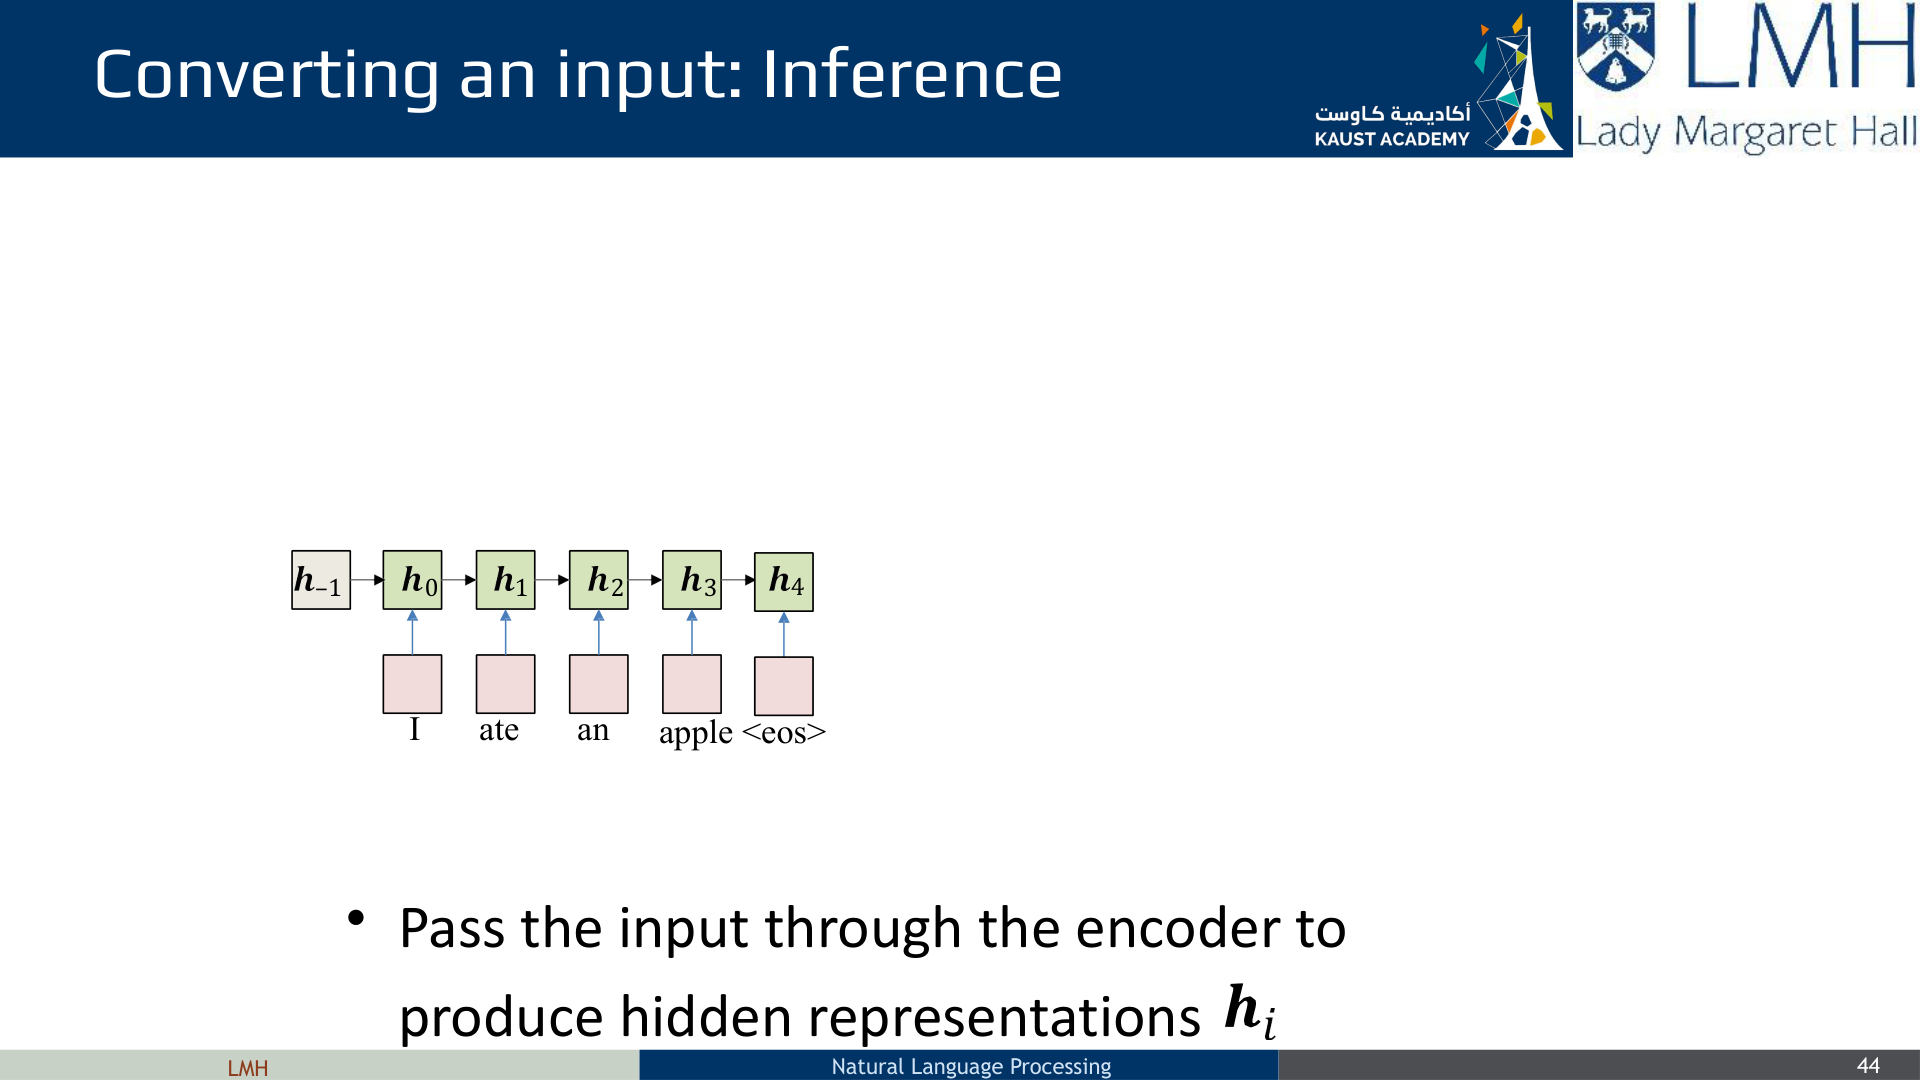
\includegraphics[width=\paperwidth,height=0.95\paperheight,keepaspectratio]{assets/Lecture-11_Large_Reasoning_Models_and_Mixture_of_Experts_Models/pdf_page_044.png}
\end{frame}

\begin{frame}[plain]
  \centering
  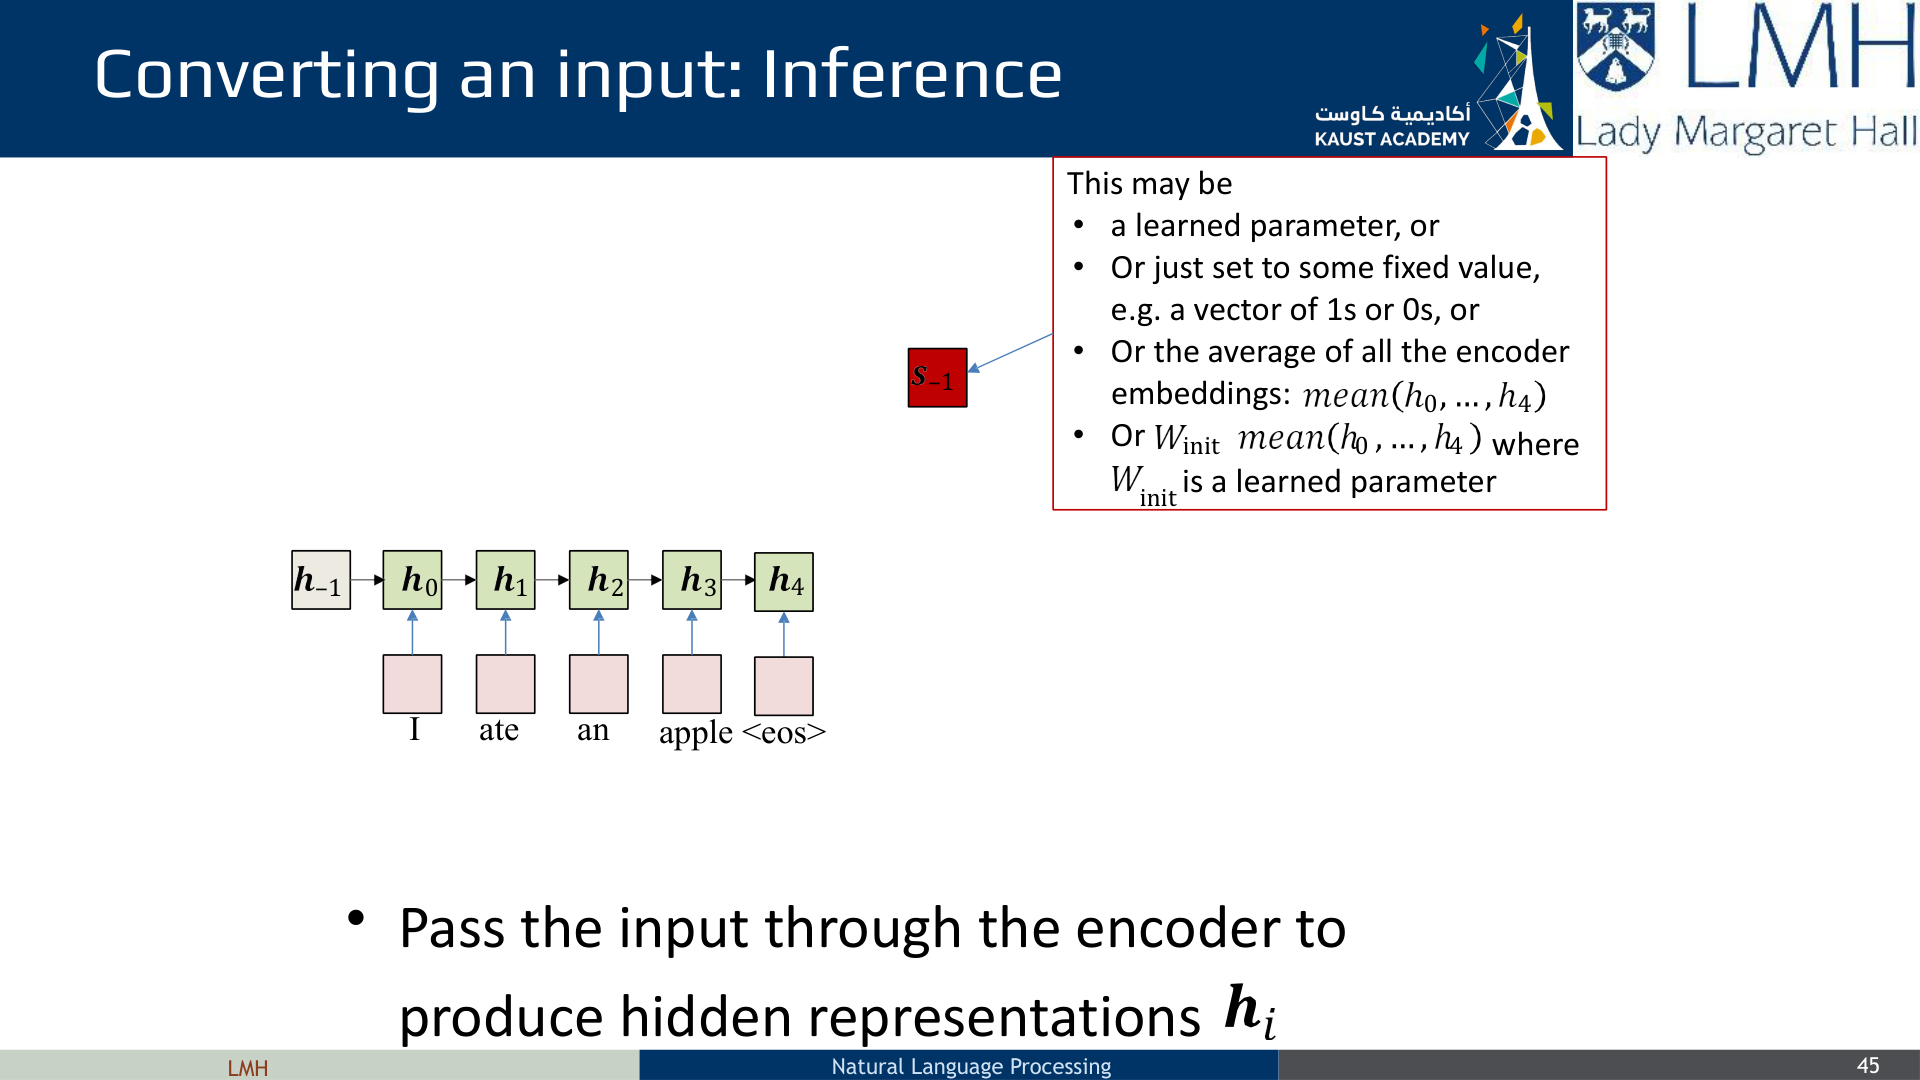
\includegraphics[width=\paperwidth,height=0.95\paperheight,keepaspectratio]{assets/Lecture-11_Large_Reasoning_Models_and_Mixture_of_Experts_Models/pdf_page_045.png}
\end{frame}

\begin{frame}[plain]
  \centering
  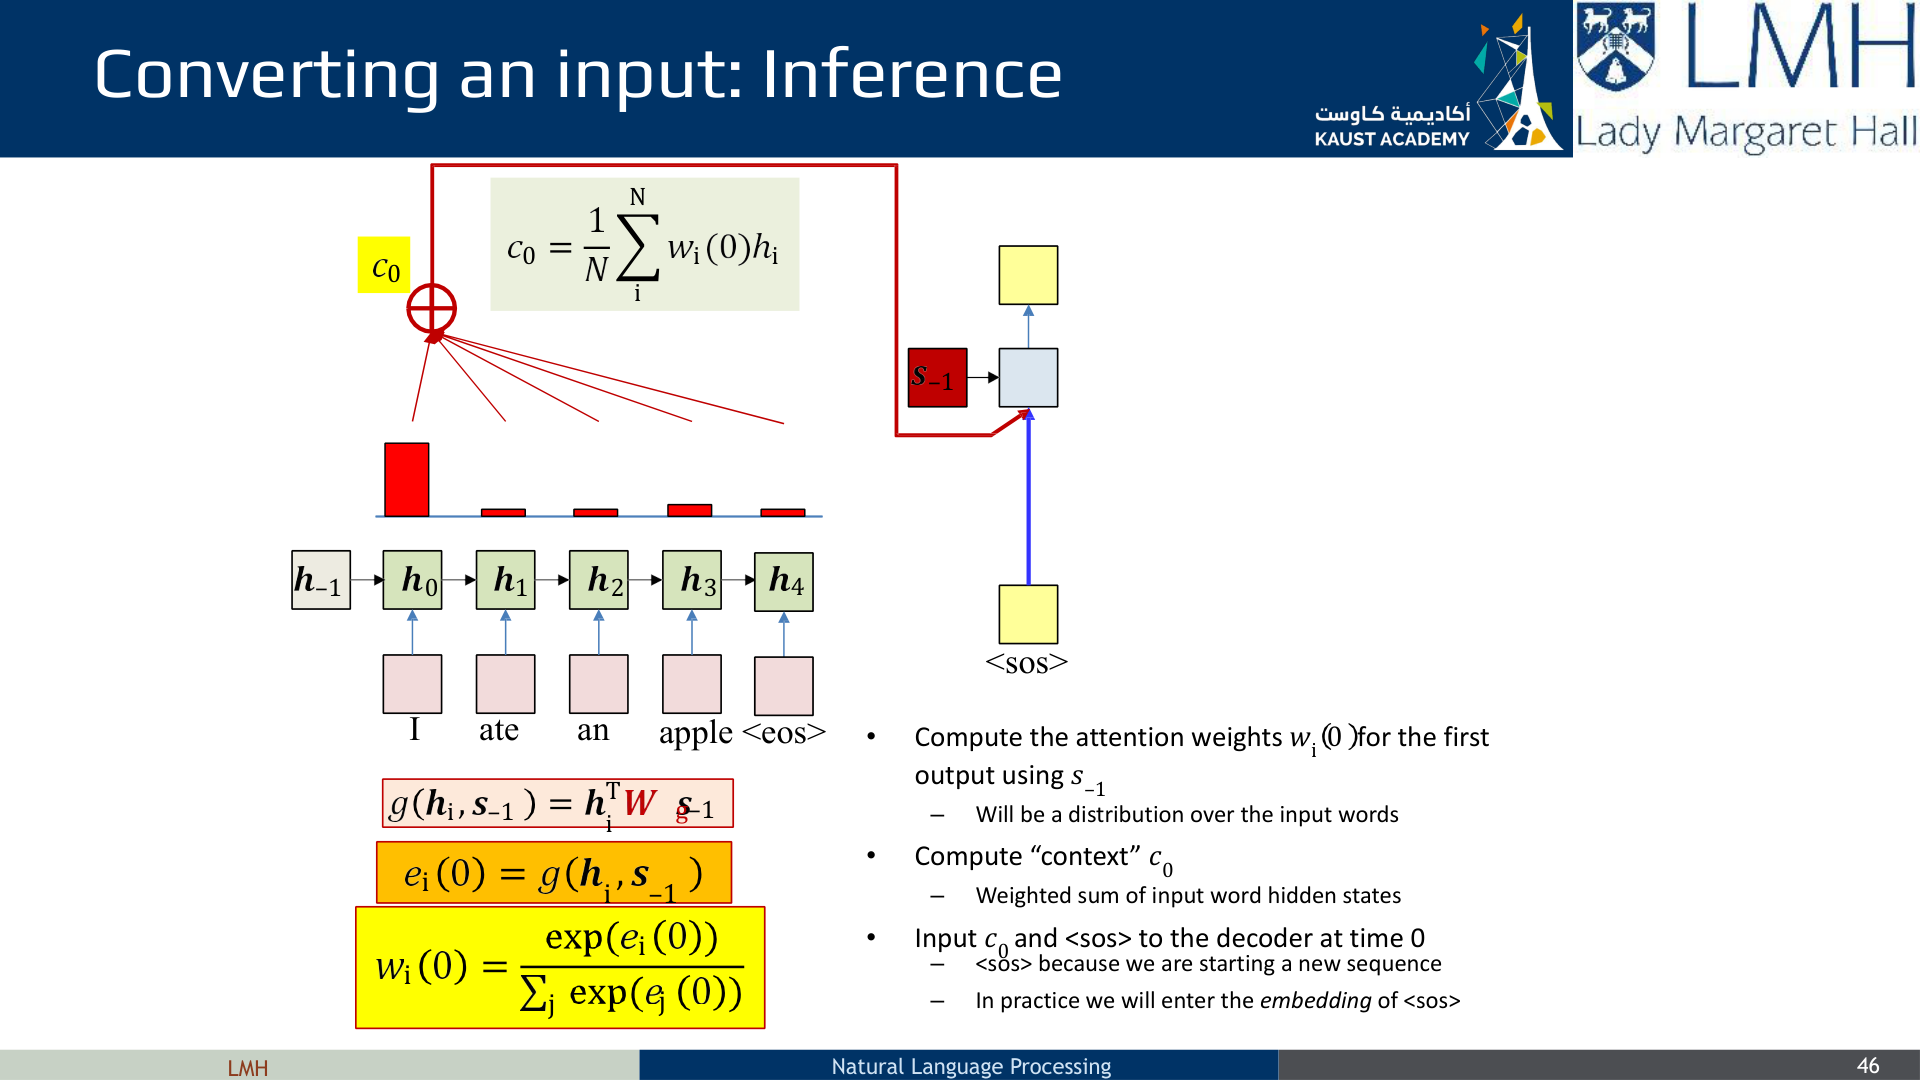
\includegraphics[width=\paperwidth,height=0.95\paperheight,keepaspectratio]{assets/Lecture-11_Large_Reasoning_Models_and_Mixture_of_Experts_Models/pdf_page_046.png}
\end{frame}

\begin{frame}[plain]
  \centering
  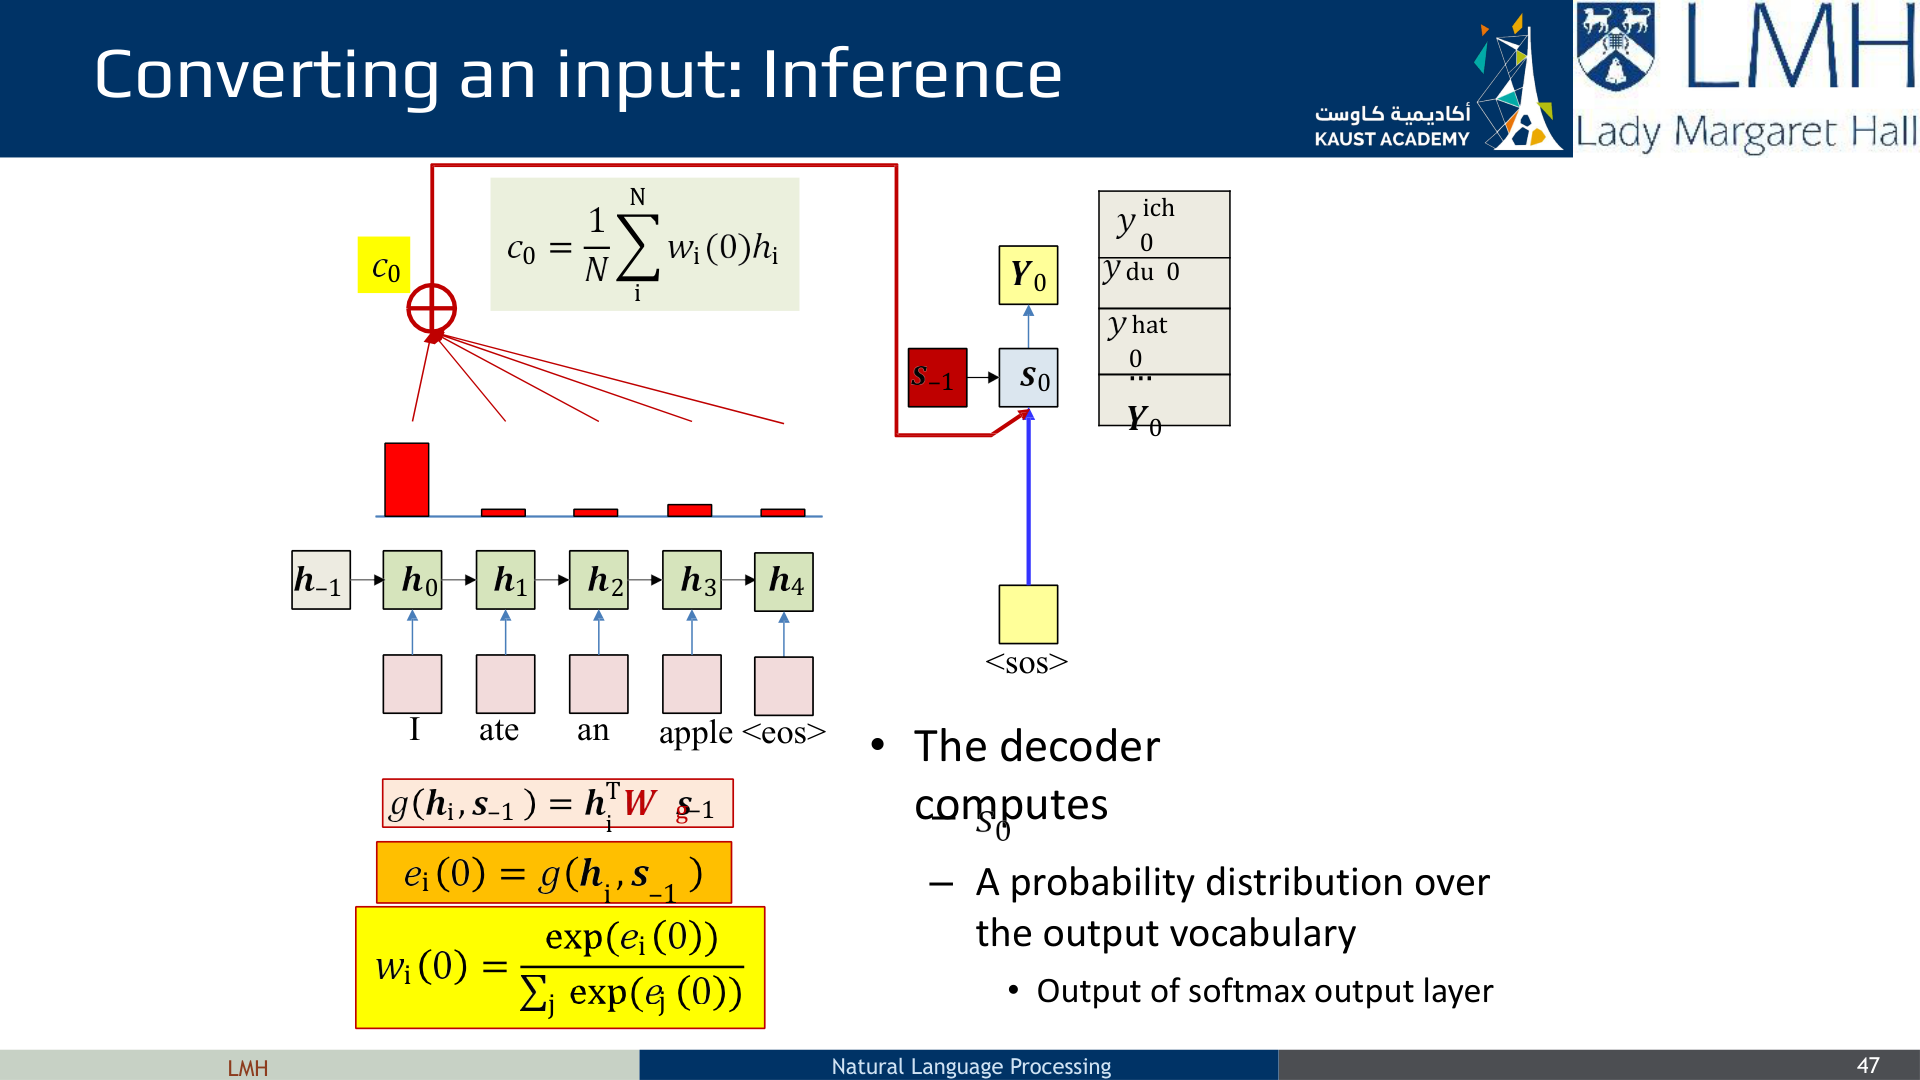
\includegraphics[width=\paperwidth,height=0.95\paperheight,keepaspectratio]{assets/Lecture-11_Large_Reasoning_Models_and_Mixture_of_Experts_Models/pdf_page_047.png}
\end{frame}

\begin{frame}[plain]
  \centering
  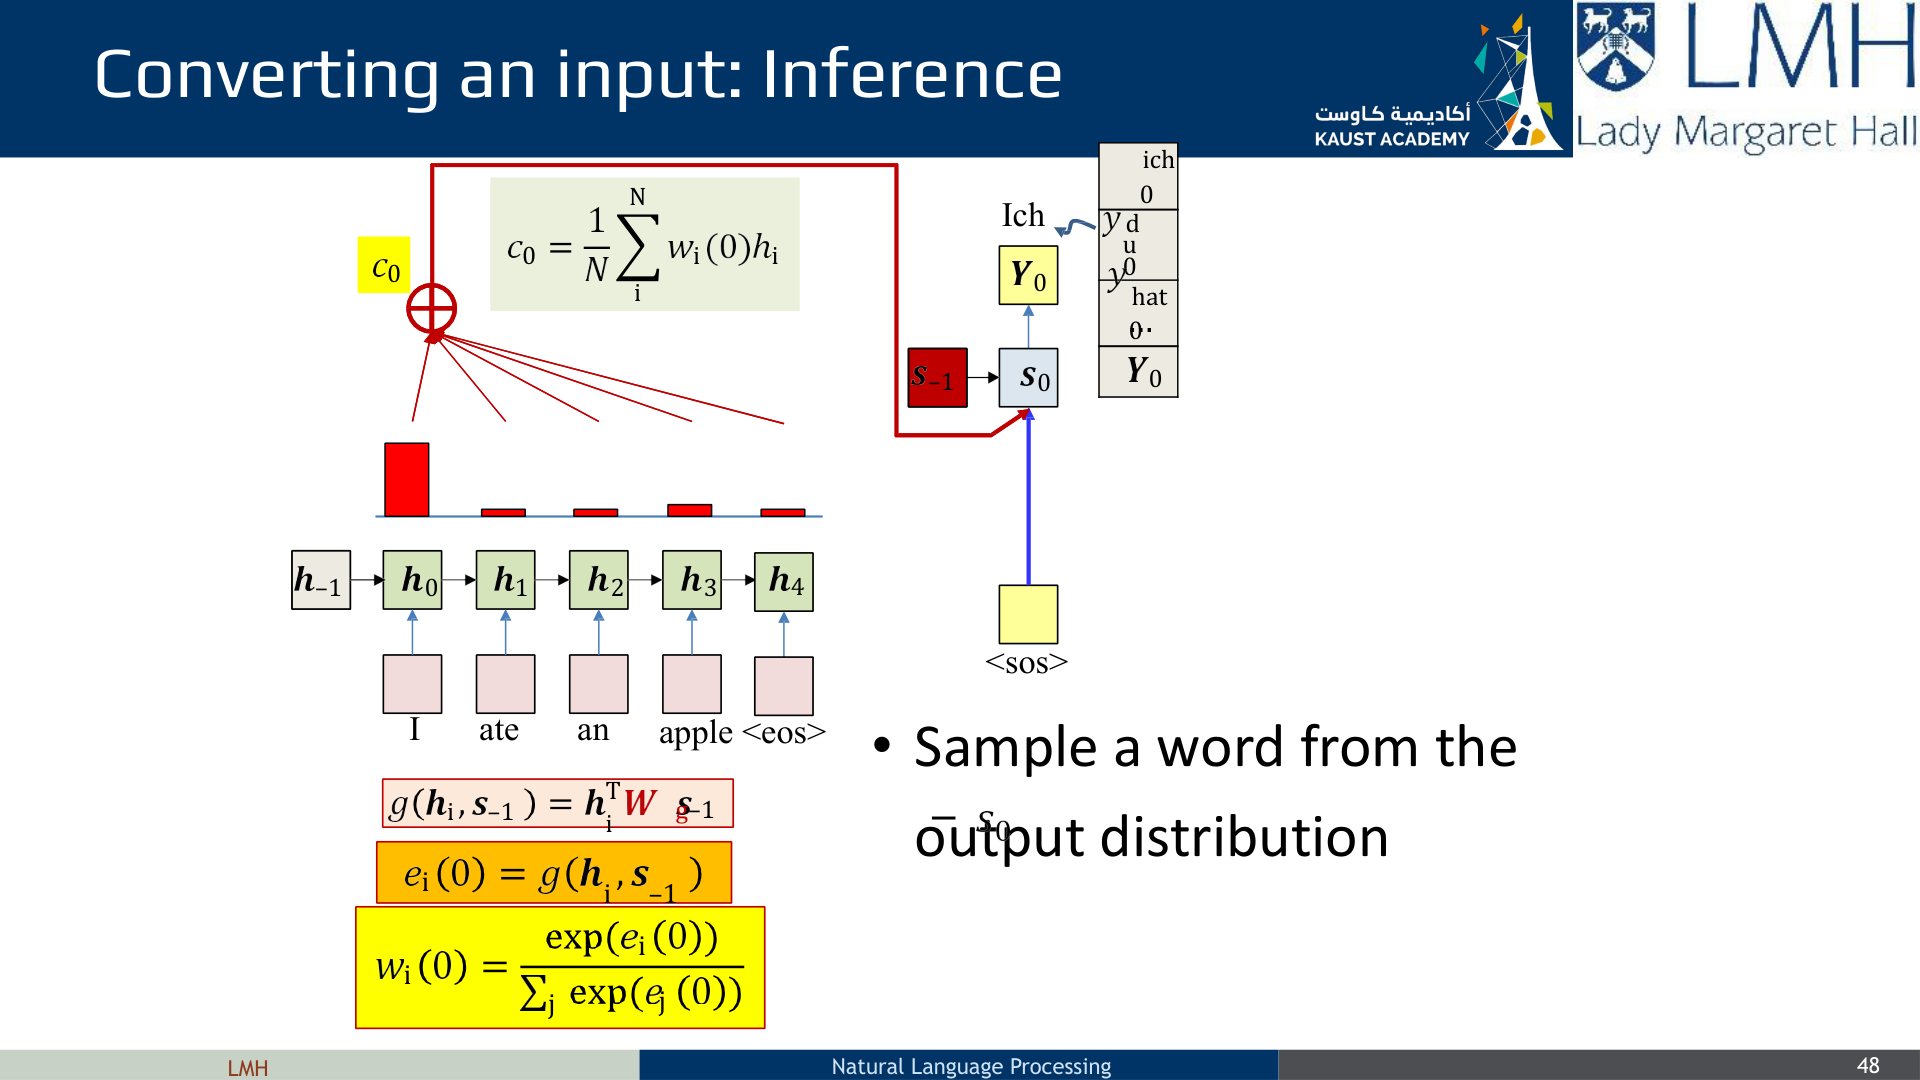
\includegraphics[width=\paperwidth,height=0.95\paperheight,keepaspectratio]{assets/Lecture-11_Large_Reasoning_Models_and_Mixture_of_Experts_Models/pdf_page_048.png}
\end{frame}

\begin{frame}[plain]
  \centering
  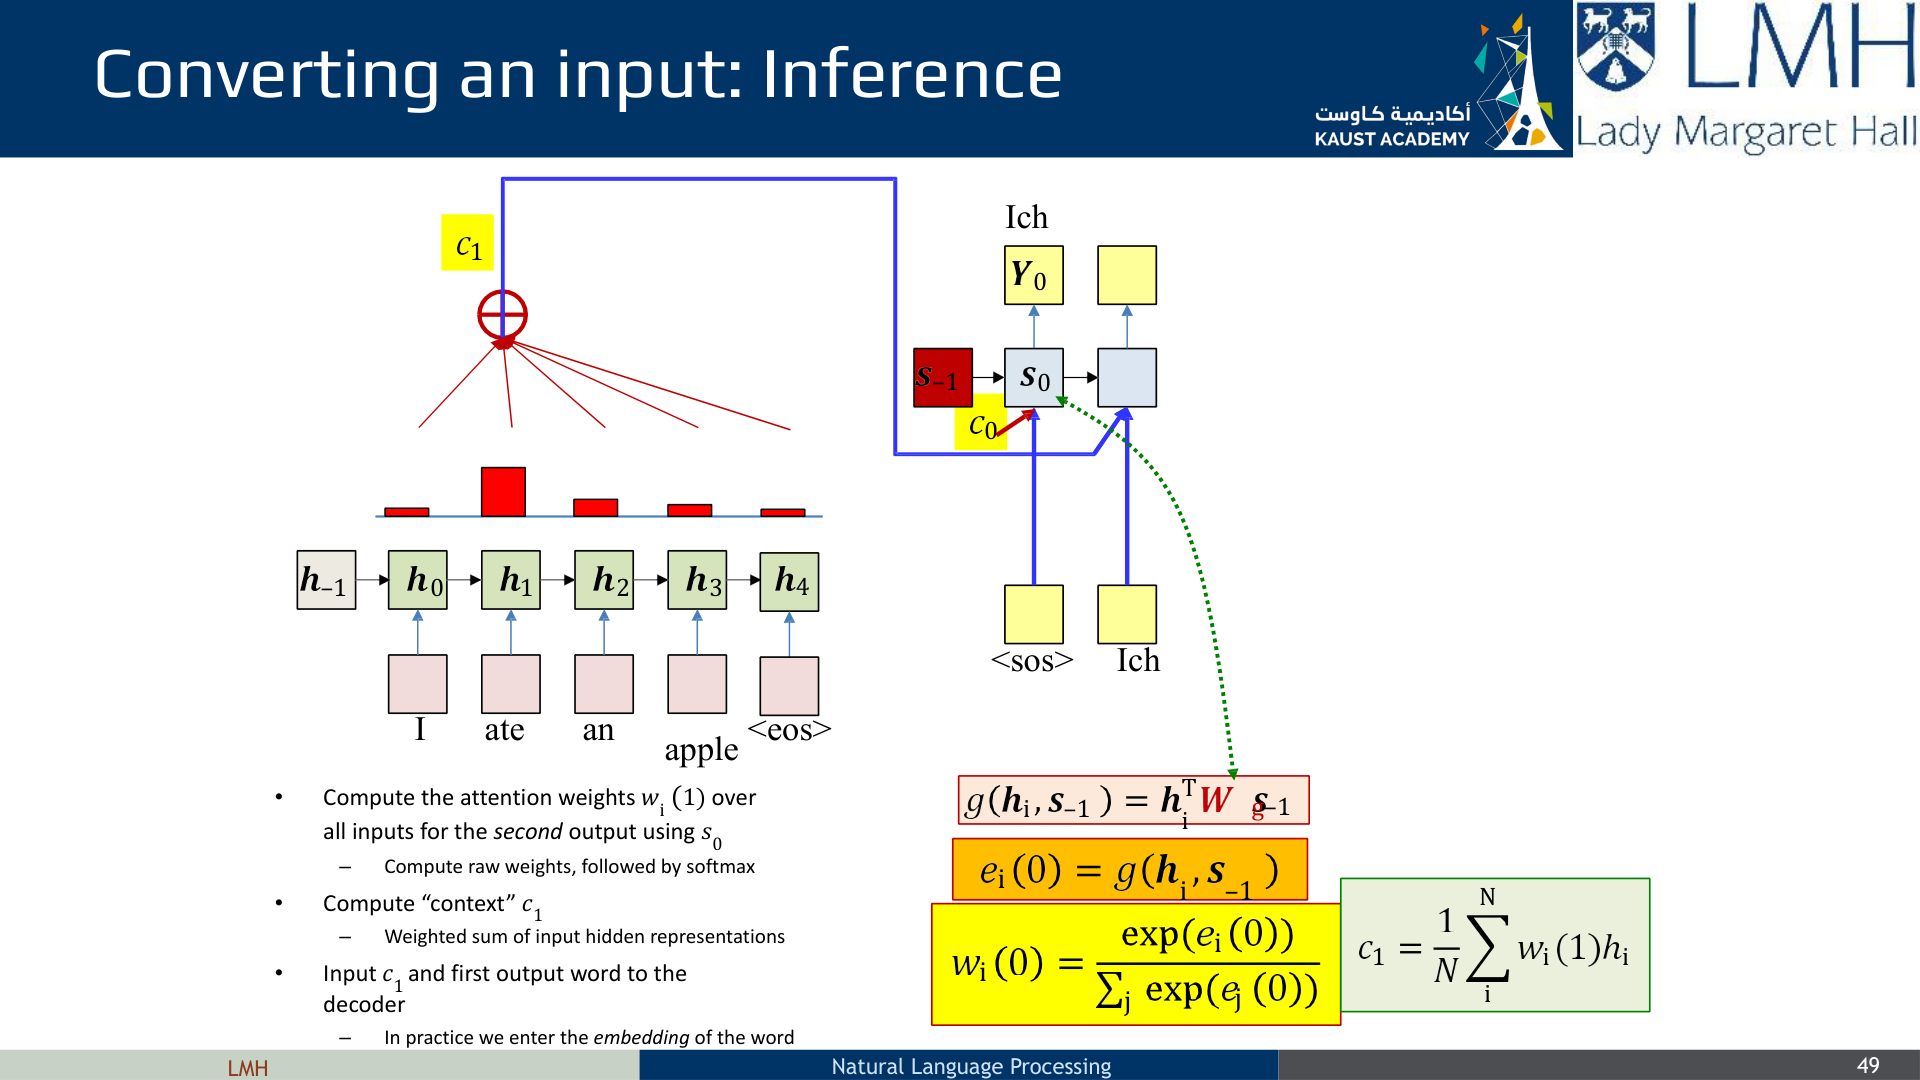
\includegraphics[width=\paperwidth,height=0.95\paperheight,keepaspectratio]{assets/Lecture-11_Large_Reasoning_Models_and_Mixture_of_Experts_Models/pdf_page_049.png}
\end{frame}

\begin{frame}[plain]
  \centering
  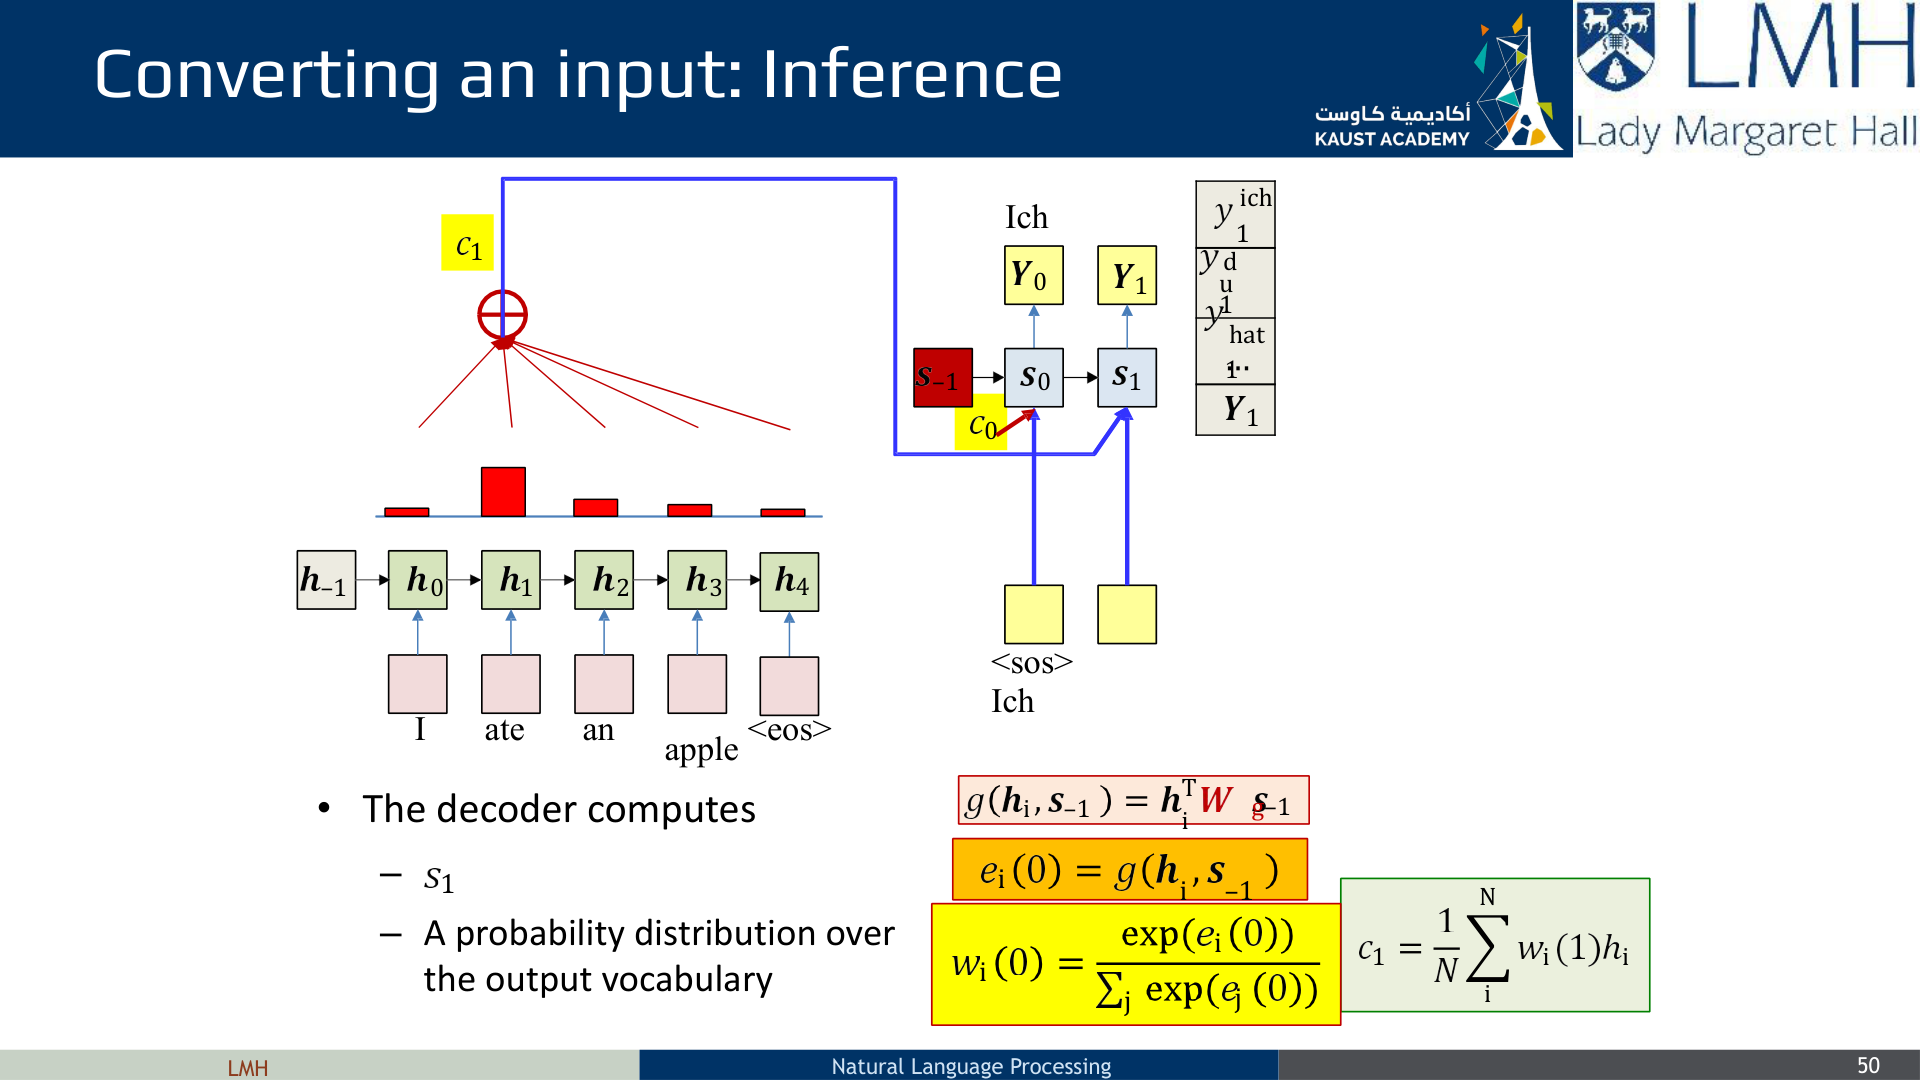
\includegraphics[width=\paperwidth,height=0.95\paperheight,keepaspectratio]{assets/Lecture-11_Large_Reasoning_Models_and_Mixture_of_Experts_Models/pdf_page_050.png}
\end{frame}

\begin{frame}[plain]
  \centering
  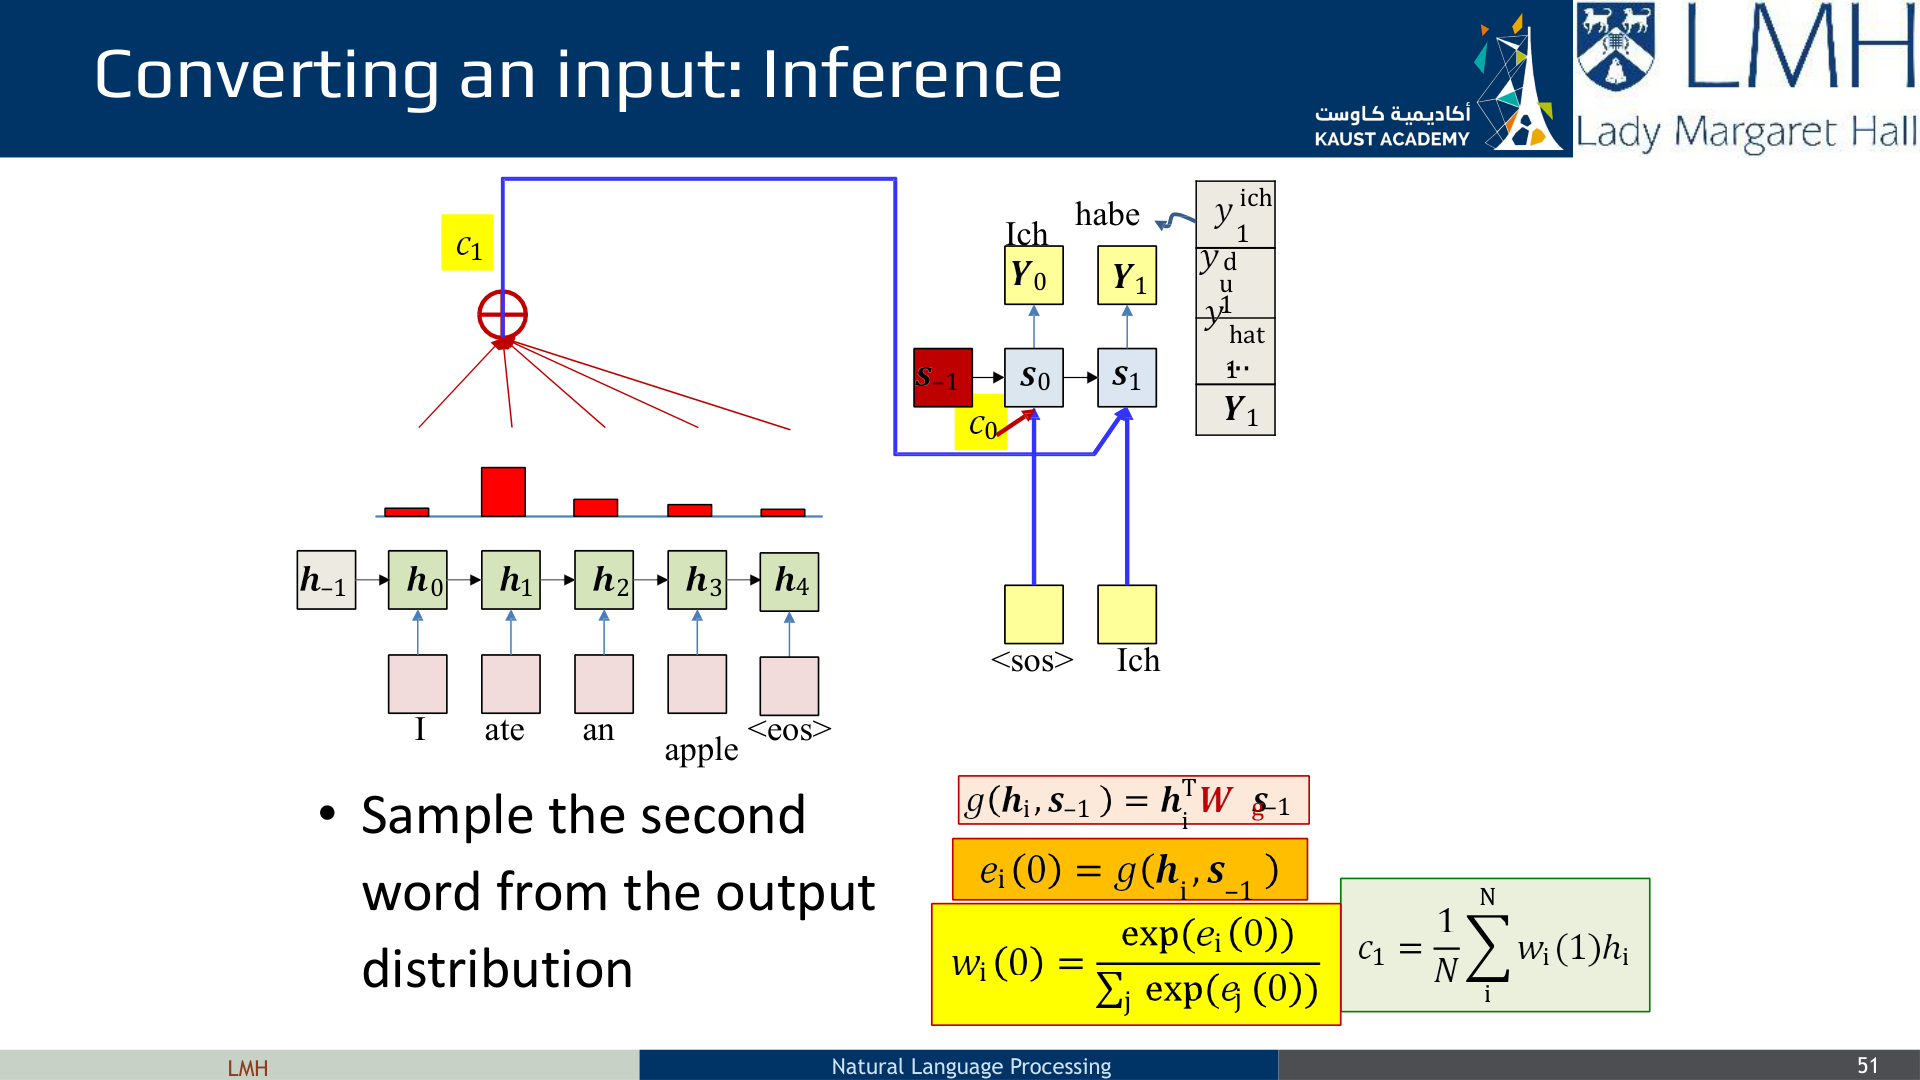
\includegraphics[width=\paperwidth,height=0.95\paperheight,keepaspectratio]{assets/Lecture-11_Large_Reasoning_Models_and_Mixture_of_Experts_Models/pdf_page_051.png}
\end{frame}

\begin{frame}[plain]
  \centering
  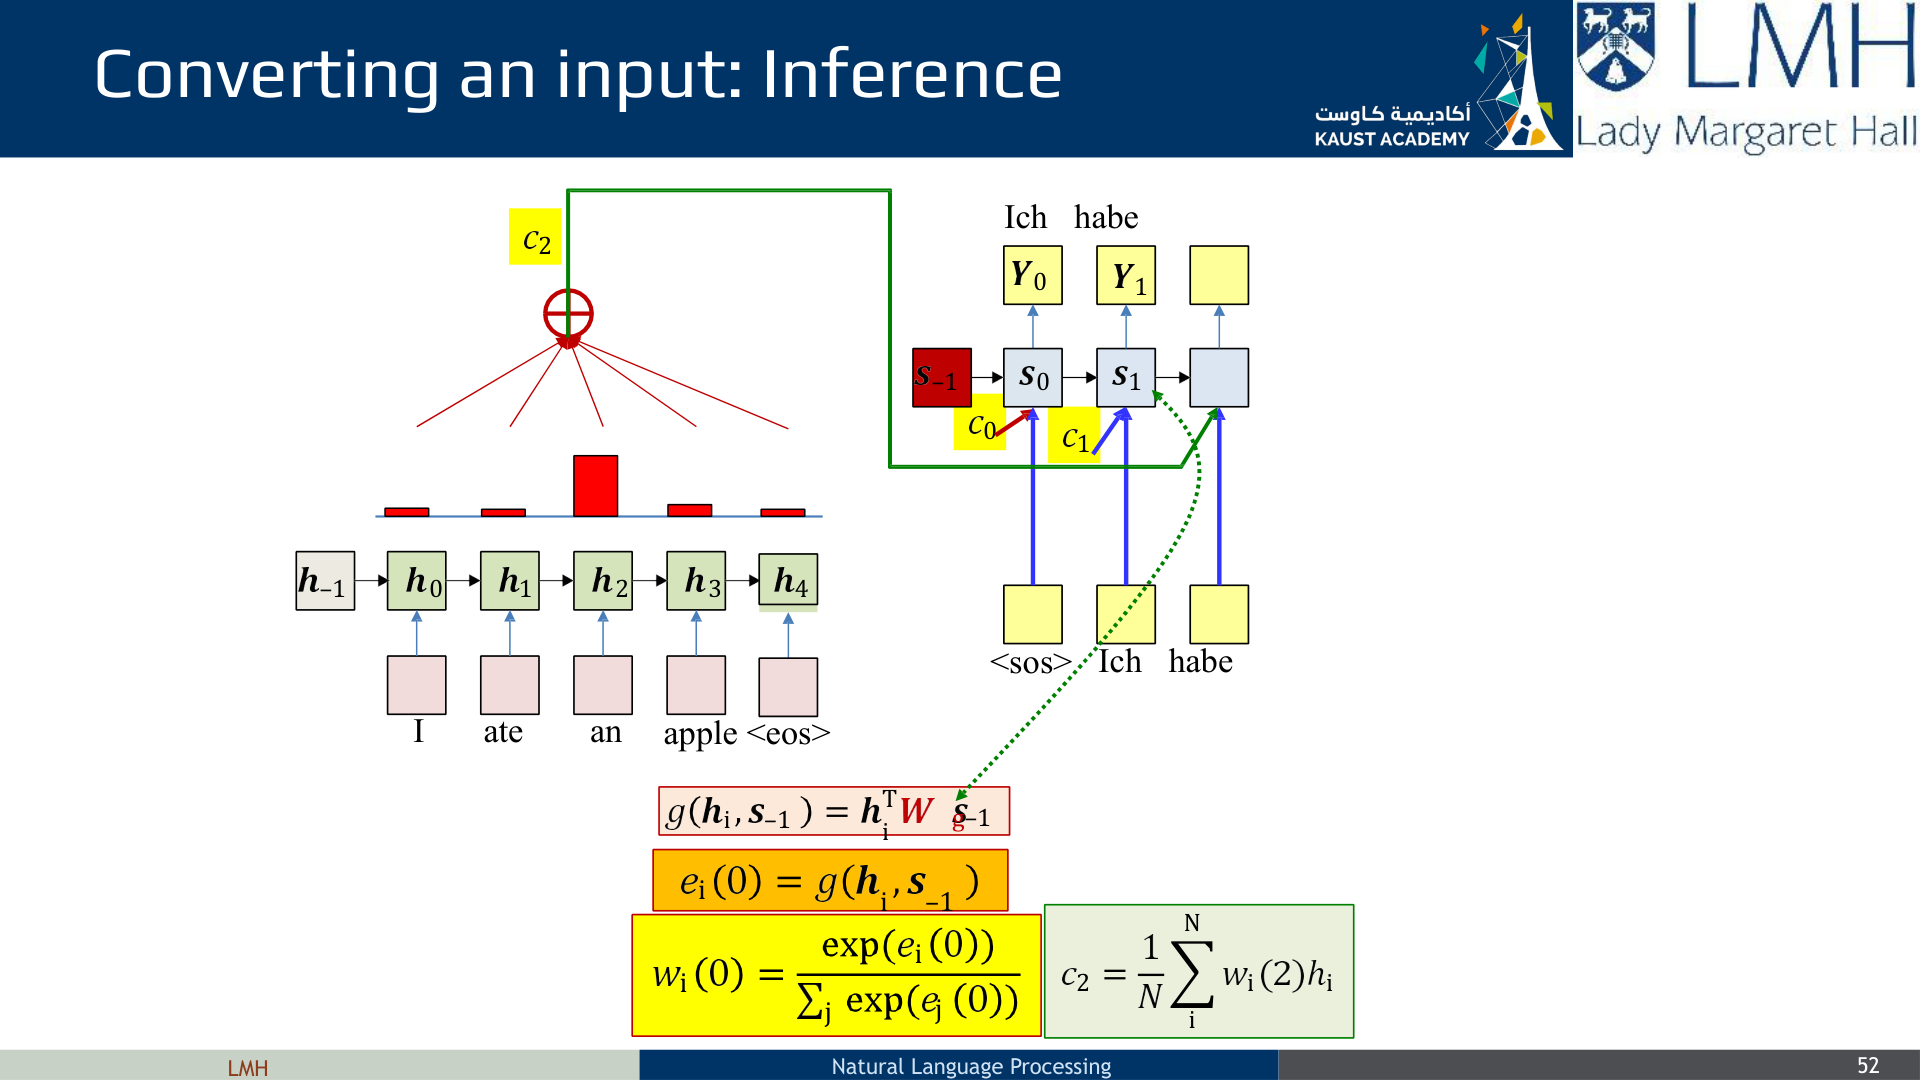
\includegraphics[width=\paperwidth,height=0.95\paperheight,keepaspectratio]{assets/Lecture-11_Large_Reasoning_Models_and_Mixture_of_Experts_Models/pdf_page_052.png}
\end{frame}

\begin{frame}[t]{Natural Language Processing}
  \begin{itemize}
    \item LMH
    \item 53
    \item Converting an input: Inference
    \item . . .
  \end{itemize}
\end{frame}

\begin{frame}[plain]
  \centering
  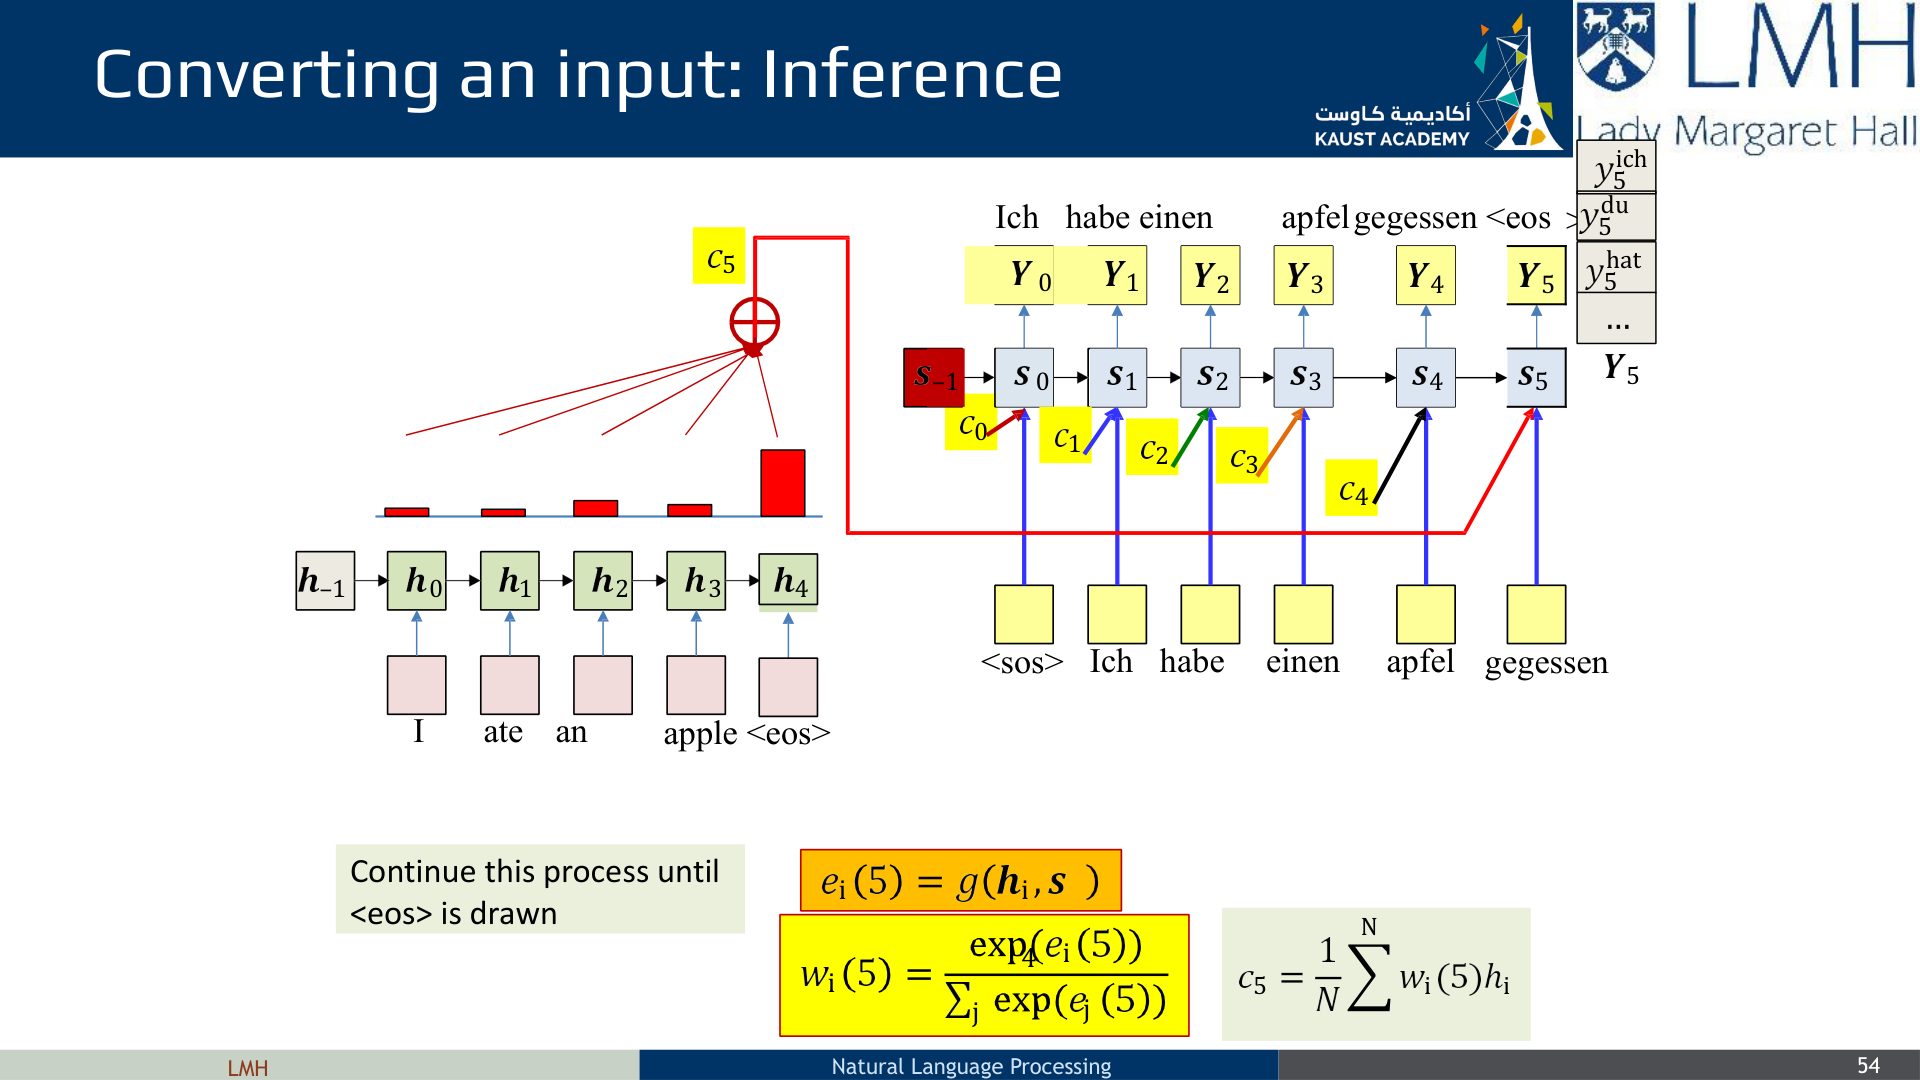
\includegraphics[width=\paperwidth,height=0.95\paperheight,keepaspectratio]{assets/Lecture-11_Large_Reasoning_Models_and_Mixture_of_Experts_Models/pdf_page_054.png}
\end{frame}

\begin{frame}[plain]
  \centering
  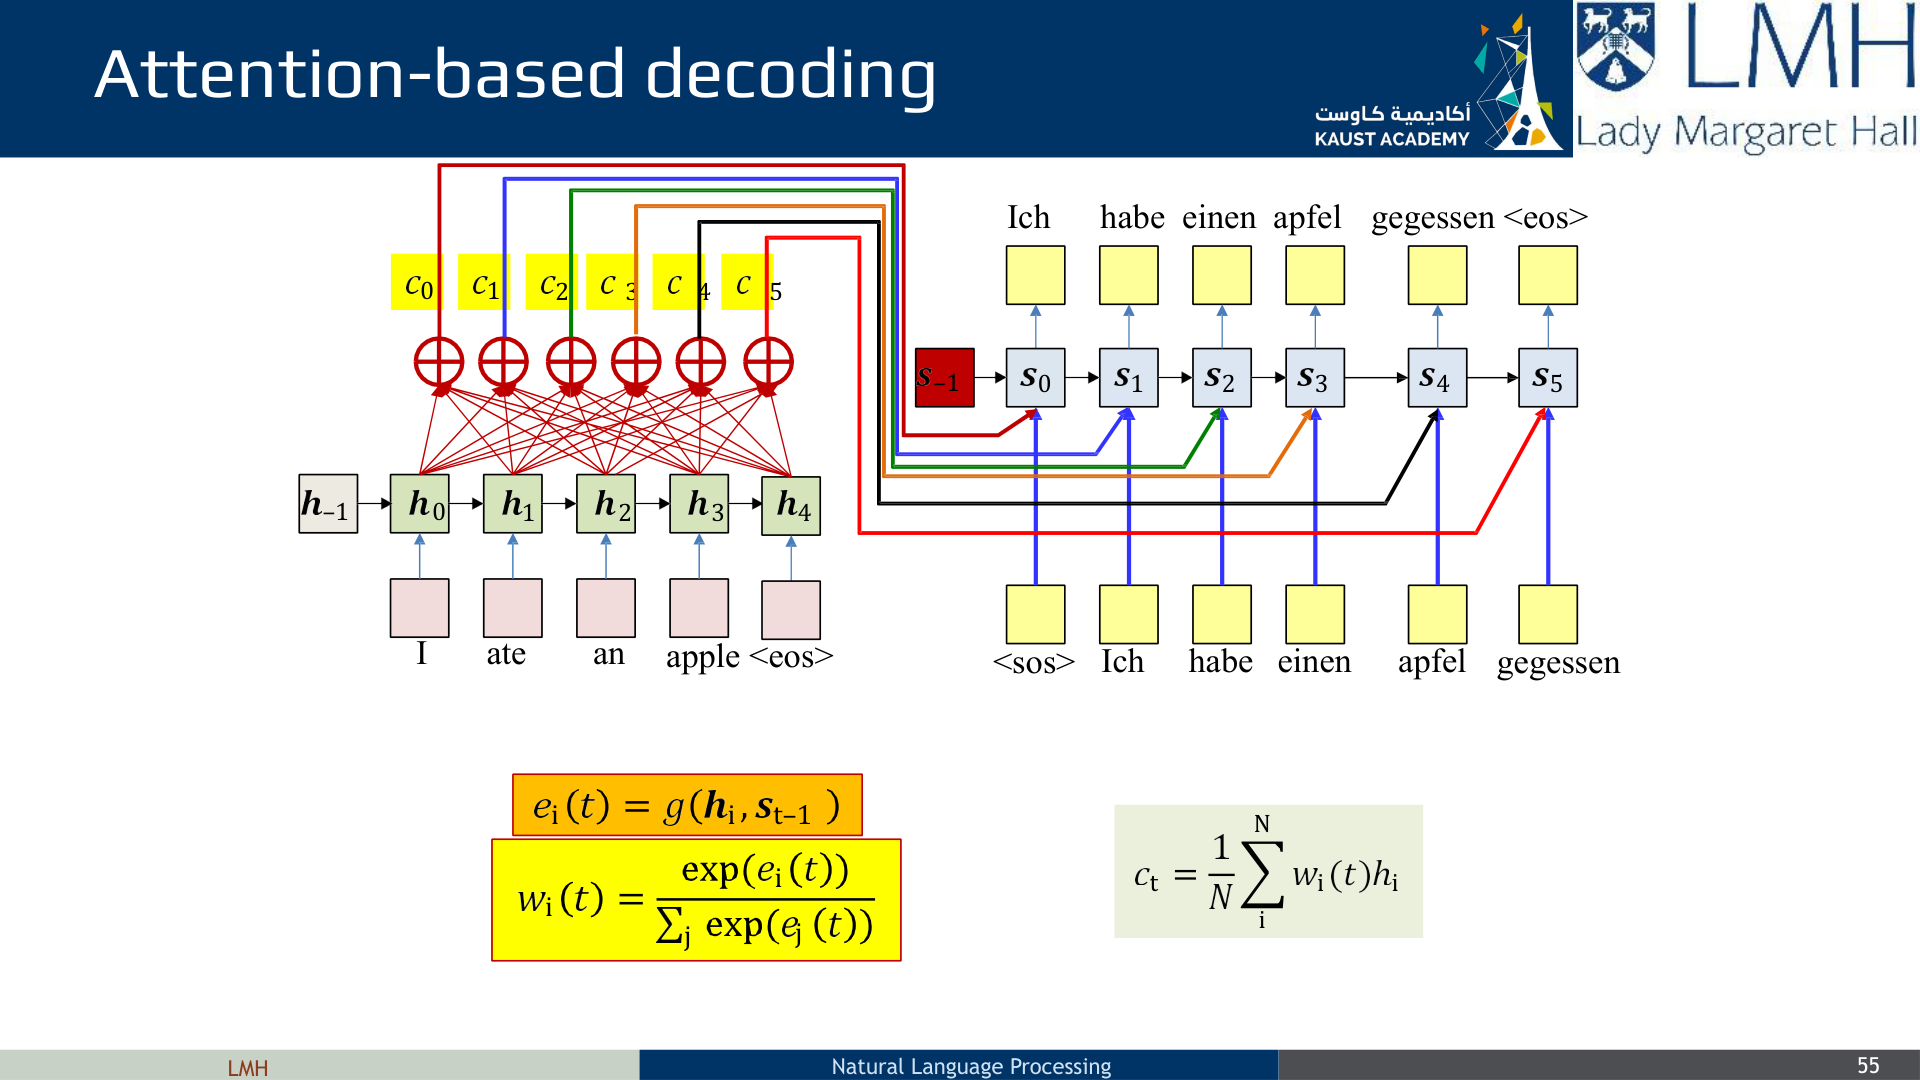
\includegraphics[width=\paperwidth,height=0.95\paperheight,keepaspectratio]{assets/Lecture-11_Large_Reasoning_Models_and_Mixture_of_Experts_Models/pdf_page_055.png}
\end{frame}

\begin{frame}[plain]
  \centering
  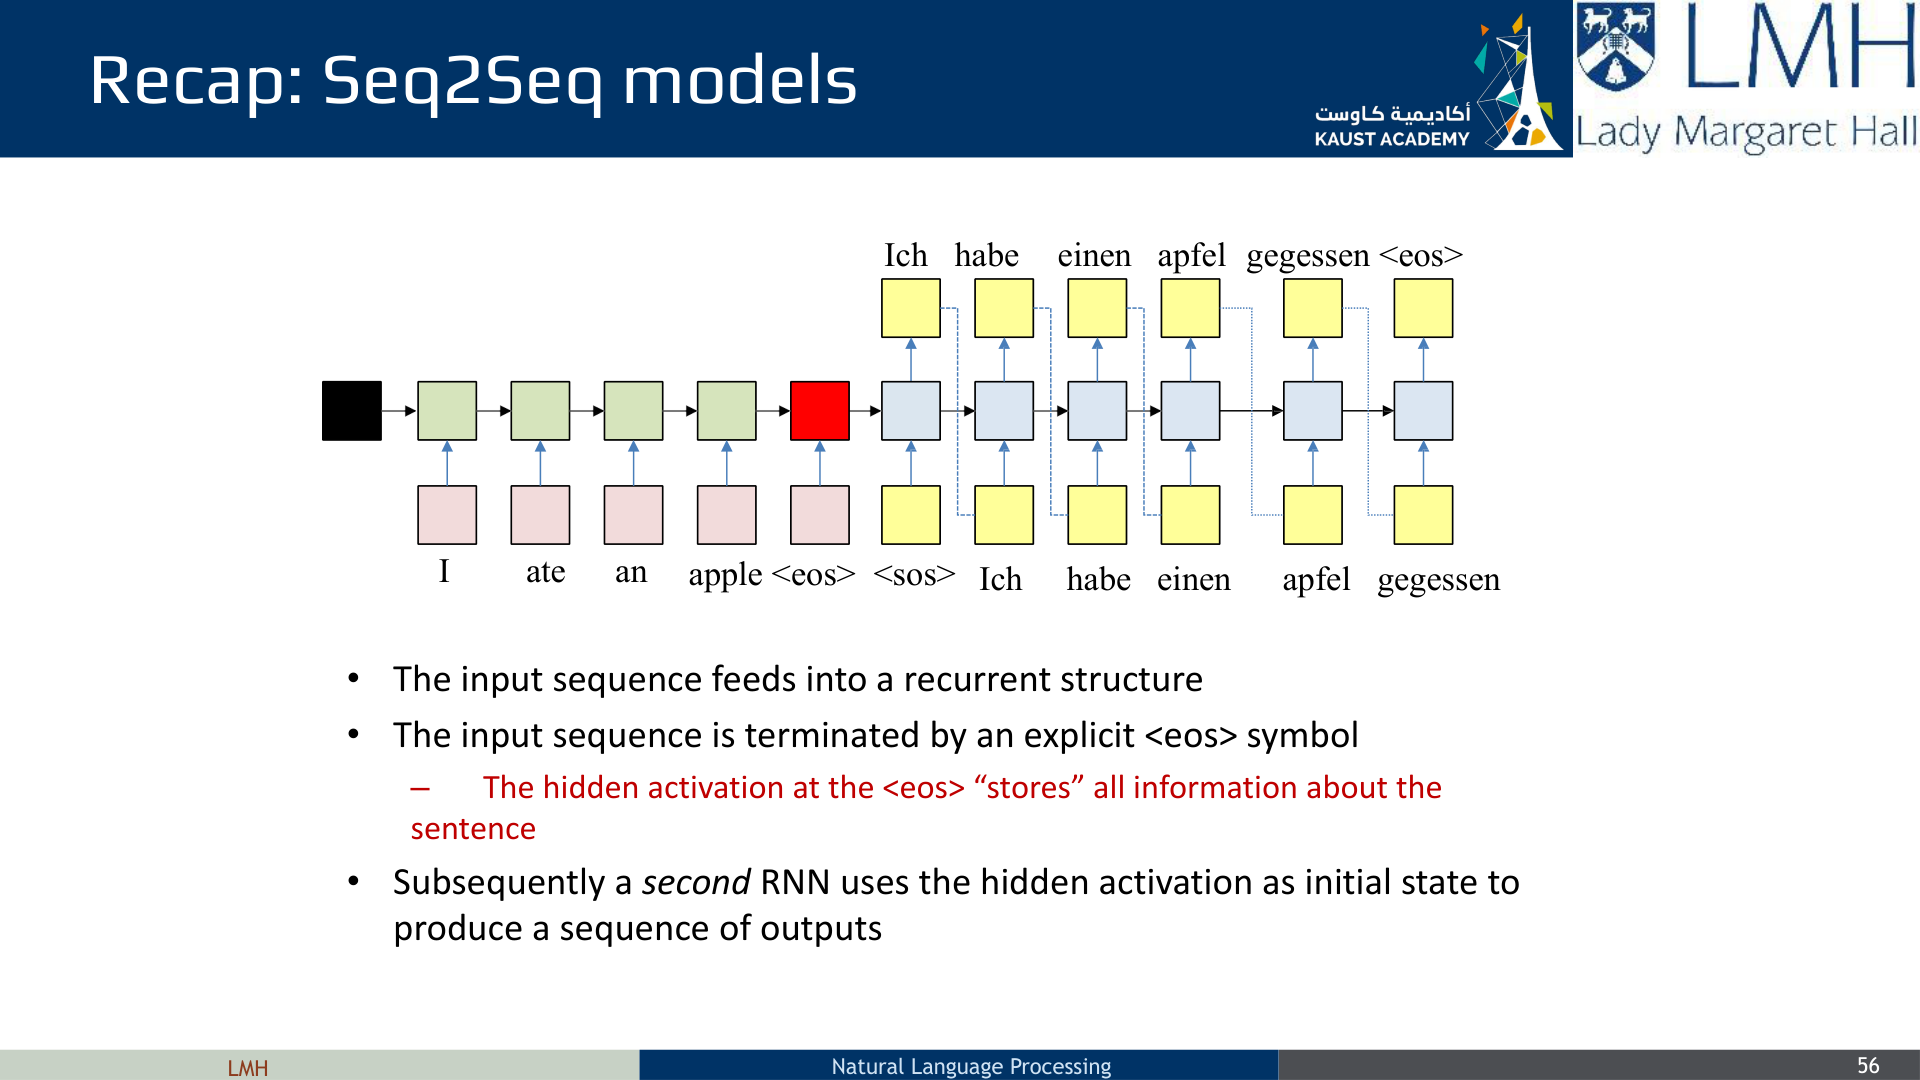
\includegraphics[width=\paperwidth,height=0.95\paperheight,keepaspectratio]{assets/Lecture-11_Large_Reasoning_Models_and_Mixture_of_Experts_Models/pdf_page_056.png}
\end{frame}

\begin{frame}[plain]
  \centering
  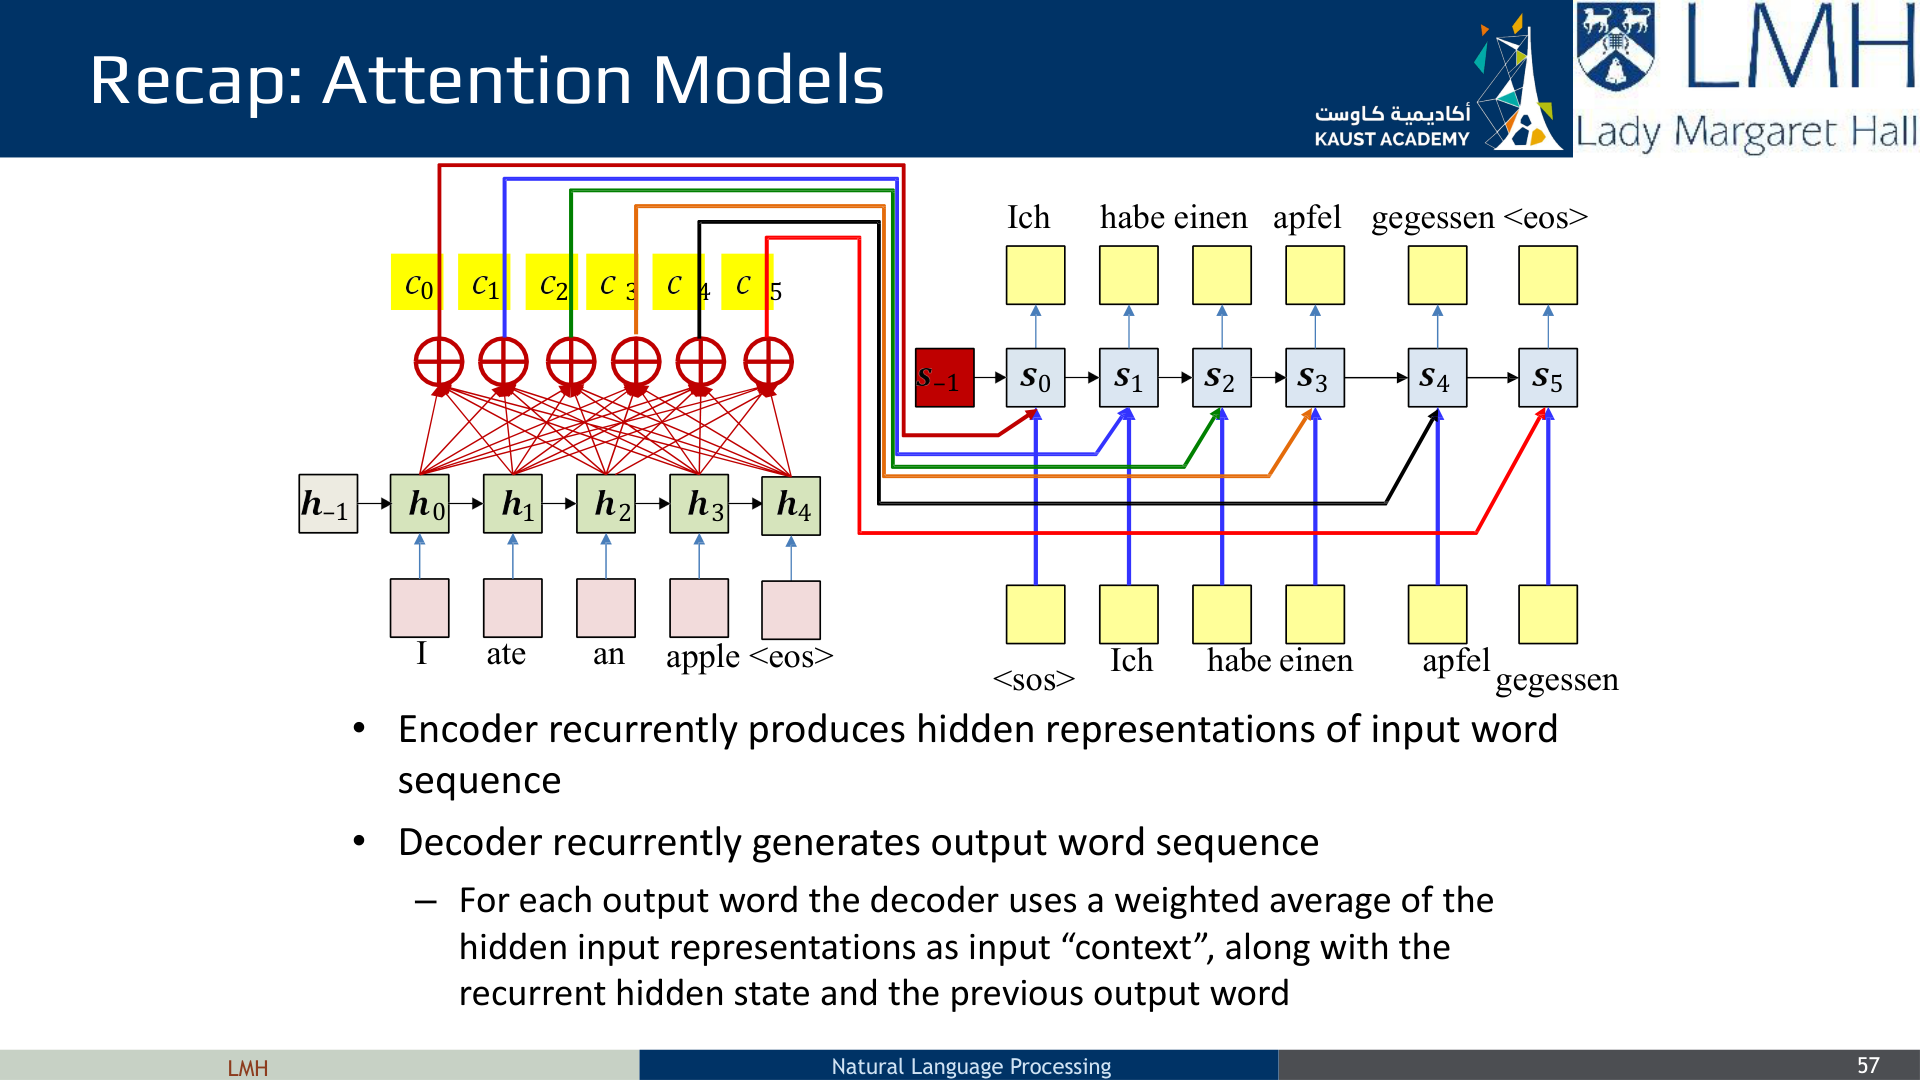
\includegraphics[width=\paperwidth,height=0.95\paperheight,keepaspectratio]{assets/Lecture-11_Large_Reasoning_Models_and_Mixture_of_Experts_Models/pdf_page_057.png}
\end{frame}

\begin{frame}[plain]
  \centering
  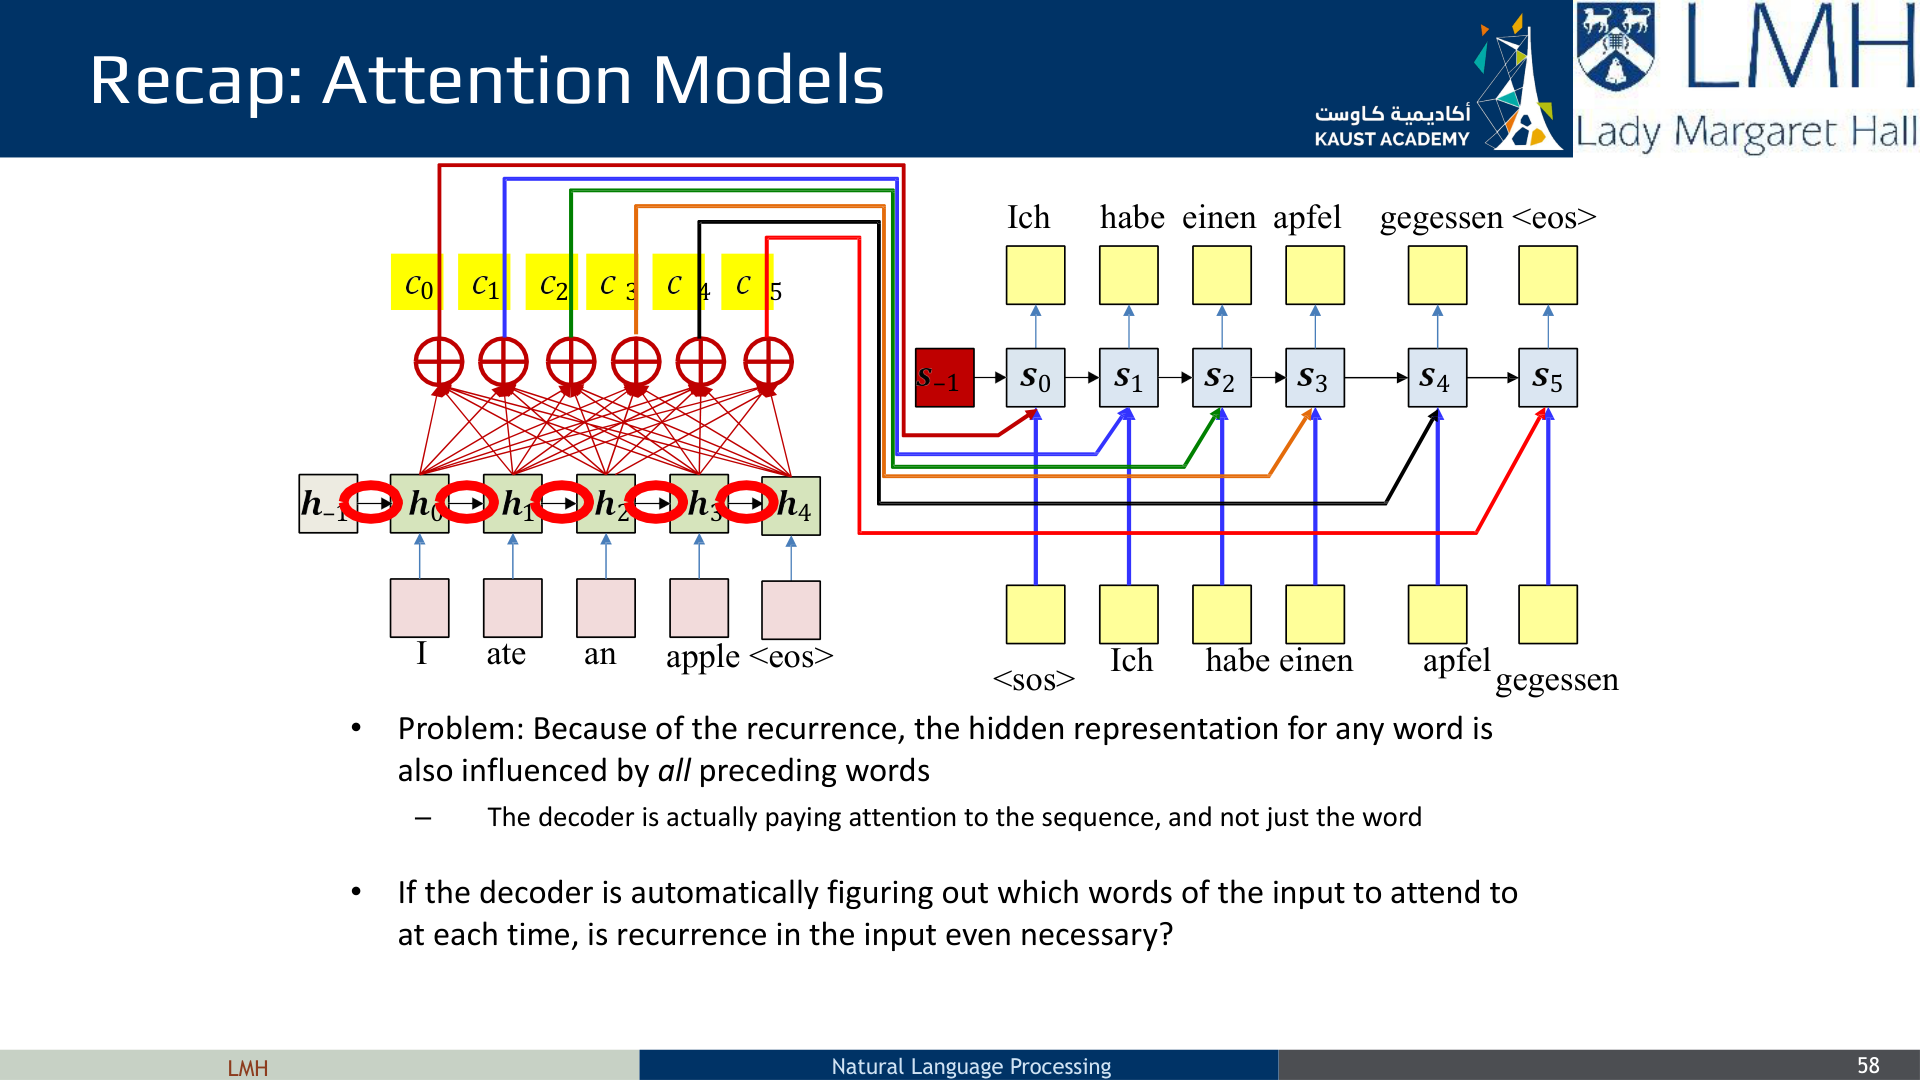
\includegraphics[width=\paperwidth,height=0.95\paperheight,keepaspectratio]{assets/Lecture-11_Large_Reasoning_Models_and_Mixture_of_Experts_Models/pdf_page_058.png}
\end{frame}

\begin{frame}[t]{Natural Language Processing}
  \begin{itemize}
    \item LMH
    \item 59
    \item Impact of Attention
  \end{itemize}
\end{frame}

\begin{frame}[t]{Natural Language Processing}
  \begin{itemize}
    \item LMH
    \item 60
    \item Limitations
  \end{itemize}
\end{frame}

\begin{frame}[t]{Natural Language Processing}
  \begin{itemize}
    \item LMH
    \item 61
    \item Future Directions
  \end{itemize}
\end{frame}

\begin{frame}[plain]
  \centering
  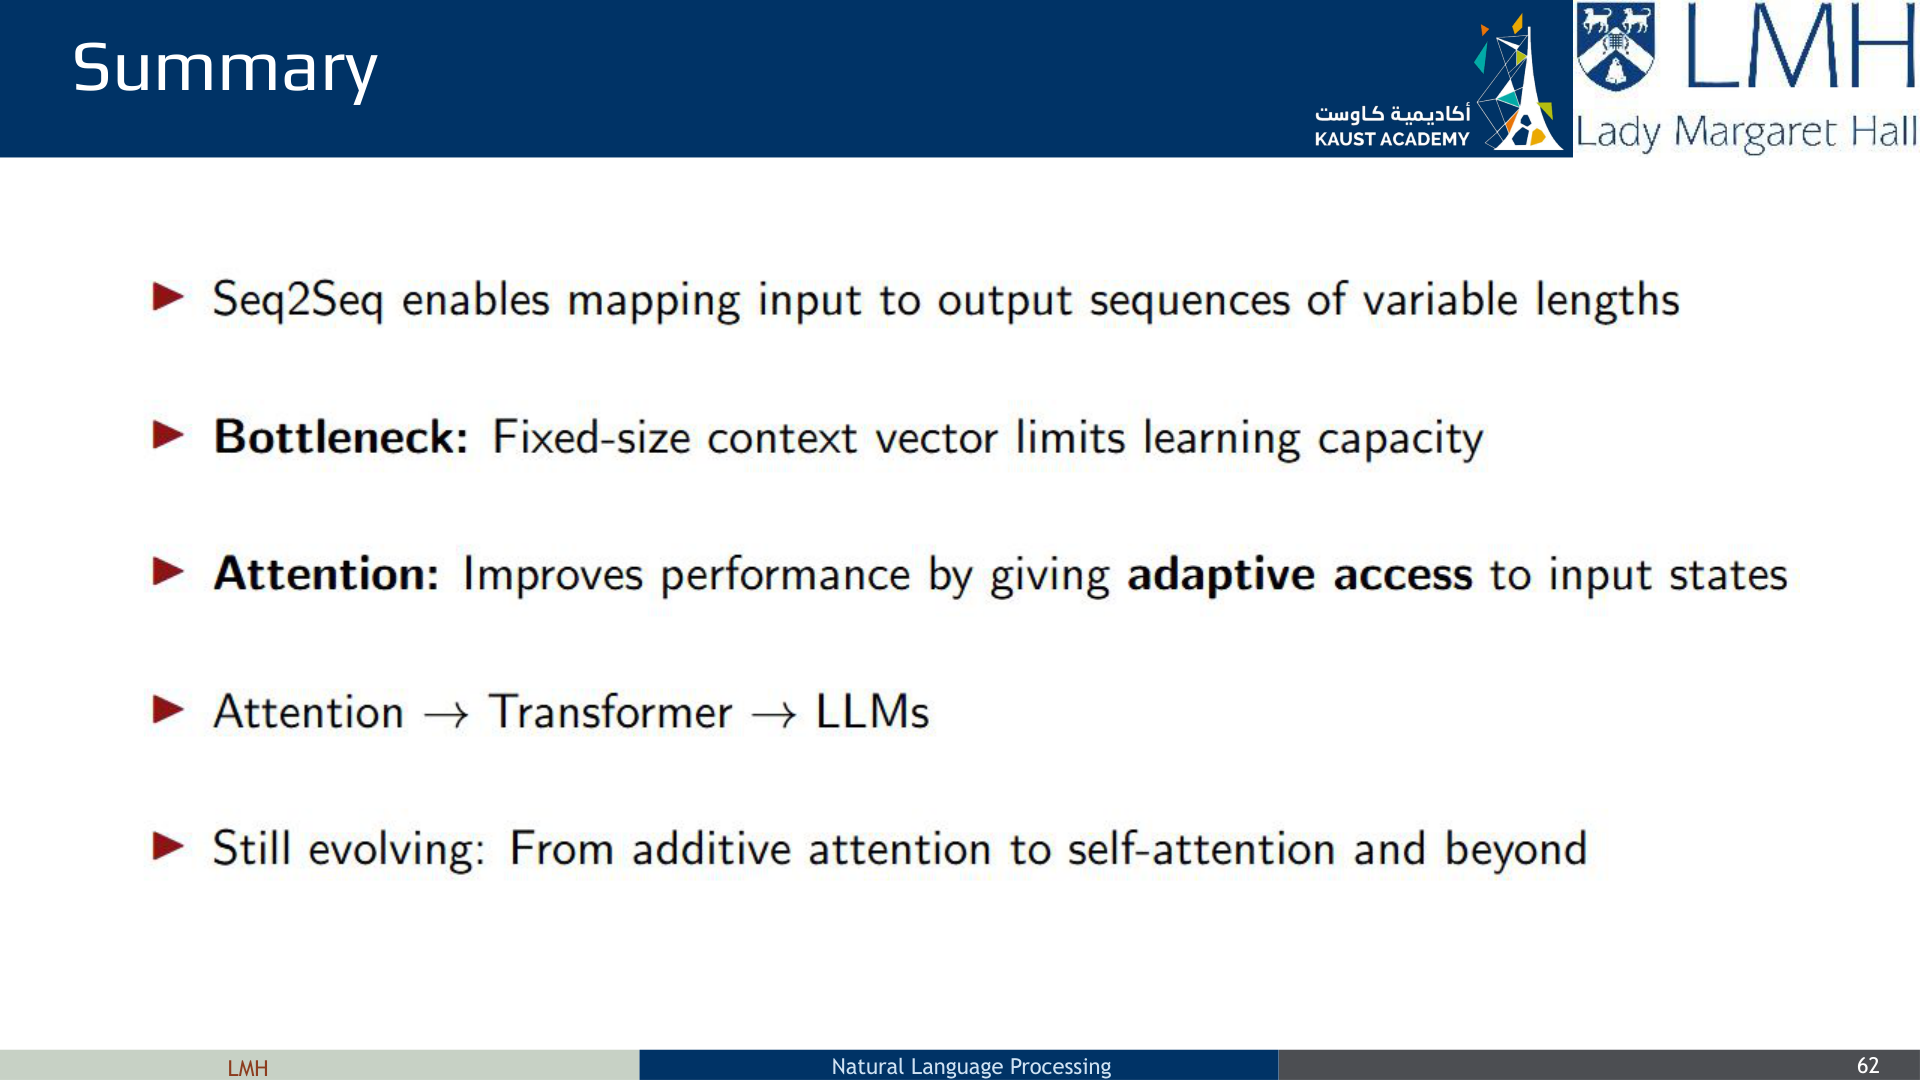
\includegraphics[width=\paperwidth,height=0.95\paperheight,keepaspectratio]{assets/Lecture-11_Large_Reasoning_Models_and_Mixture_of_Experts_Models/pdf_page_062.png}
\end{frame}

\begin{frame}[t]{Natural Language Processing}
  \begin{itemize}
    \item LMH
    \item 63
    \item References
    \item These slides have been adapted from:
    \item ->Younes Mourri \\& Lukasz Kaiser, Natural Language Processcing
    \item Specialization, DeepLearning.Ai
    \item ->Bhiksha Raj \\& Rita Singh, 11-785 Introduction to Deep Learning,
    \item CMU
  \end{itemize}
\end{frame}

\begin{frame}[plain]
  \centering
  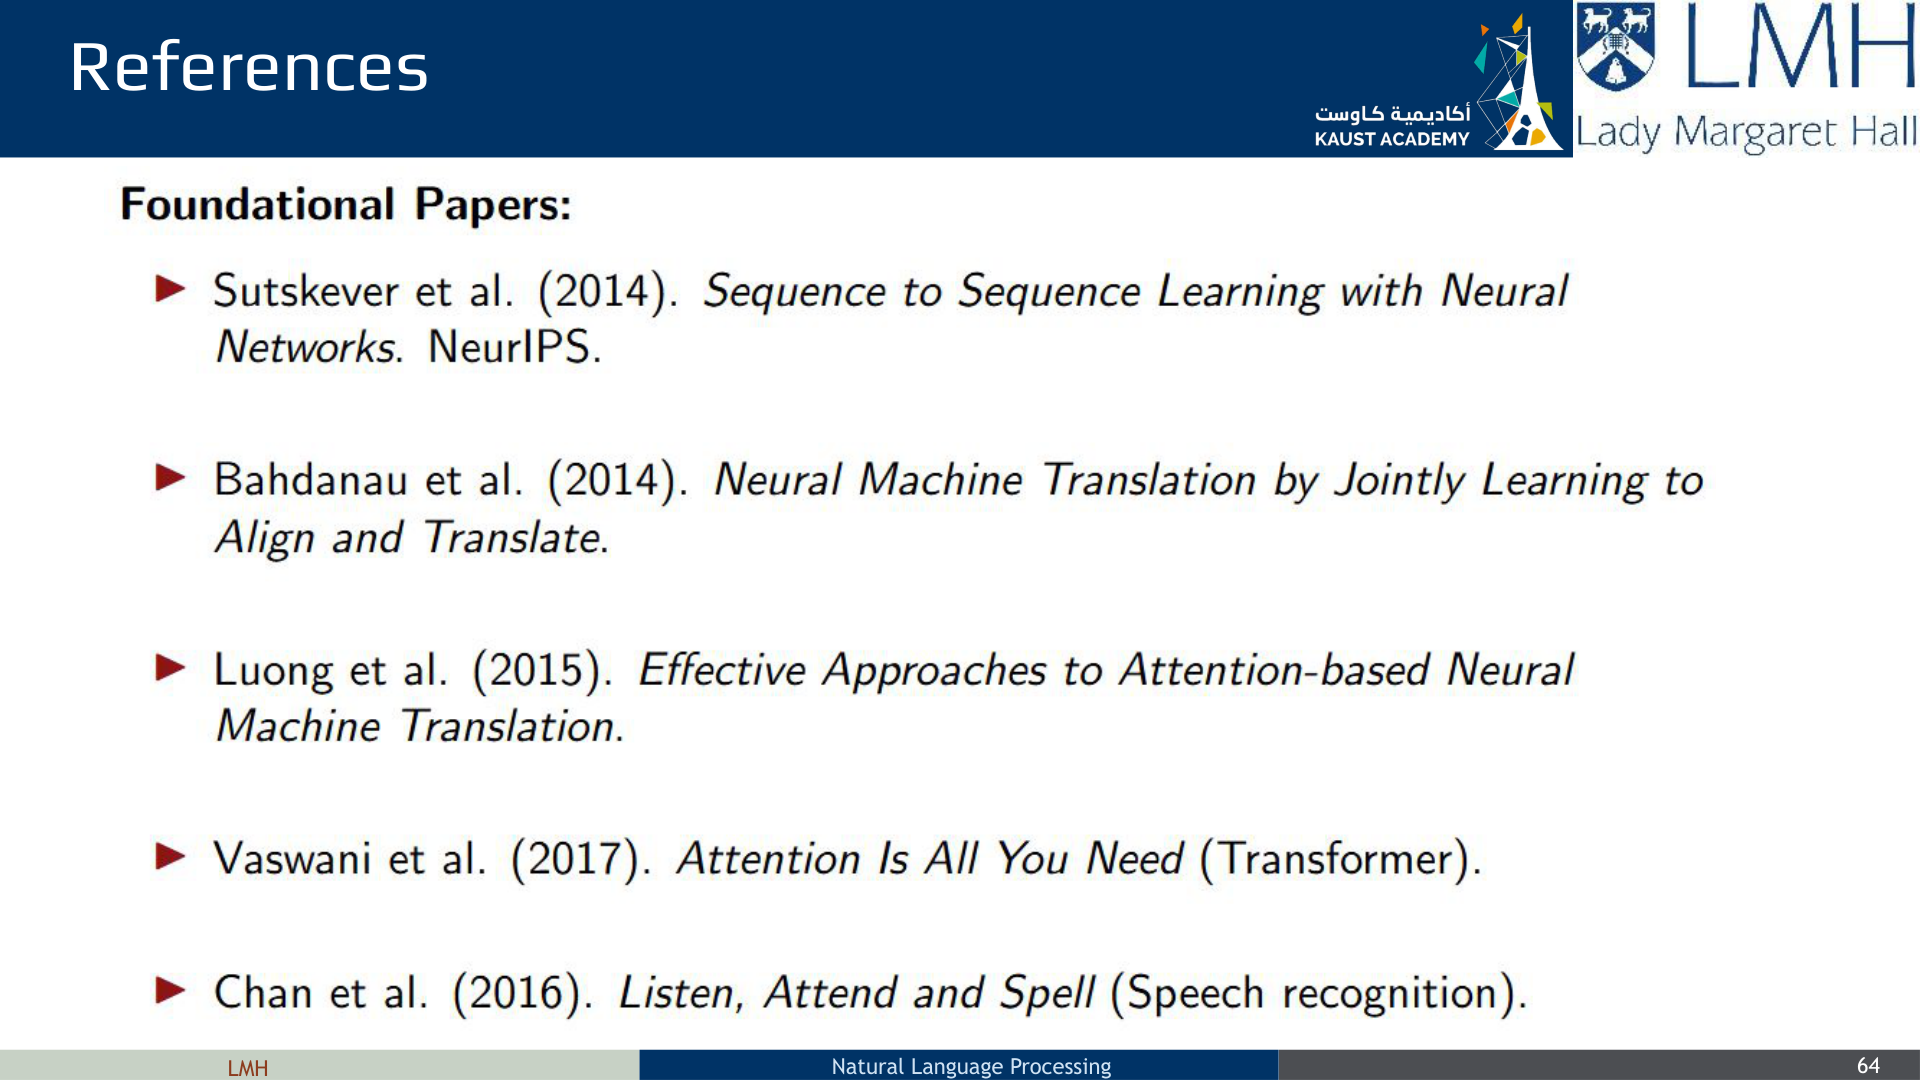
\includegraphics[width=\paperwidth,height=0.95\paperheight,keepaspectratio]{assets/Lecture-11_Large_Reasoning_Models_and_Mixture_of_Experts_Models/pdf_page_064.png}
\end{frame}

\begin{frame}[t]{Natural Language Processing}
  \begin{itemize}
    \item LMH
    \item 65
    \item References
  \end{itemize}
\end{frame}

\begin{frame}[plain]
  \centering
  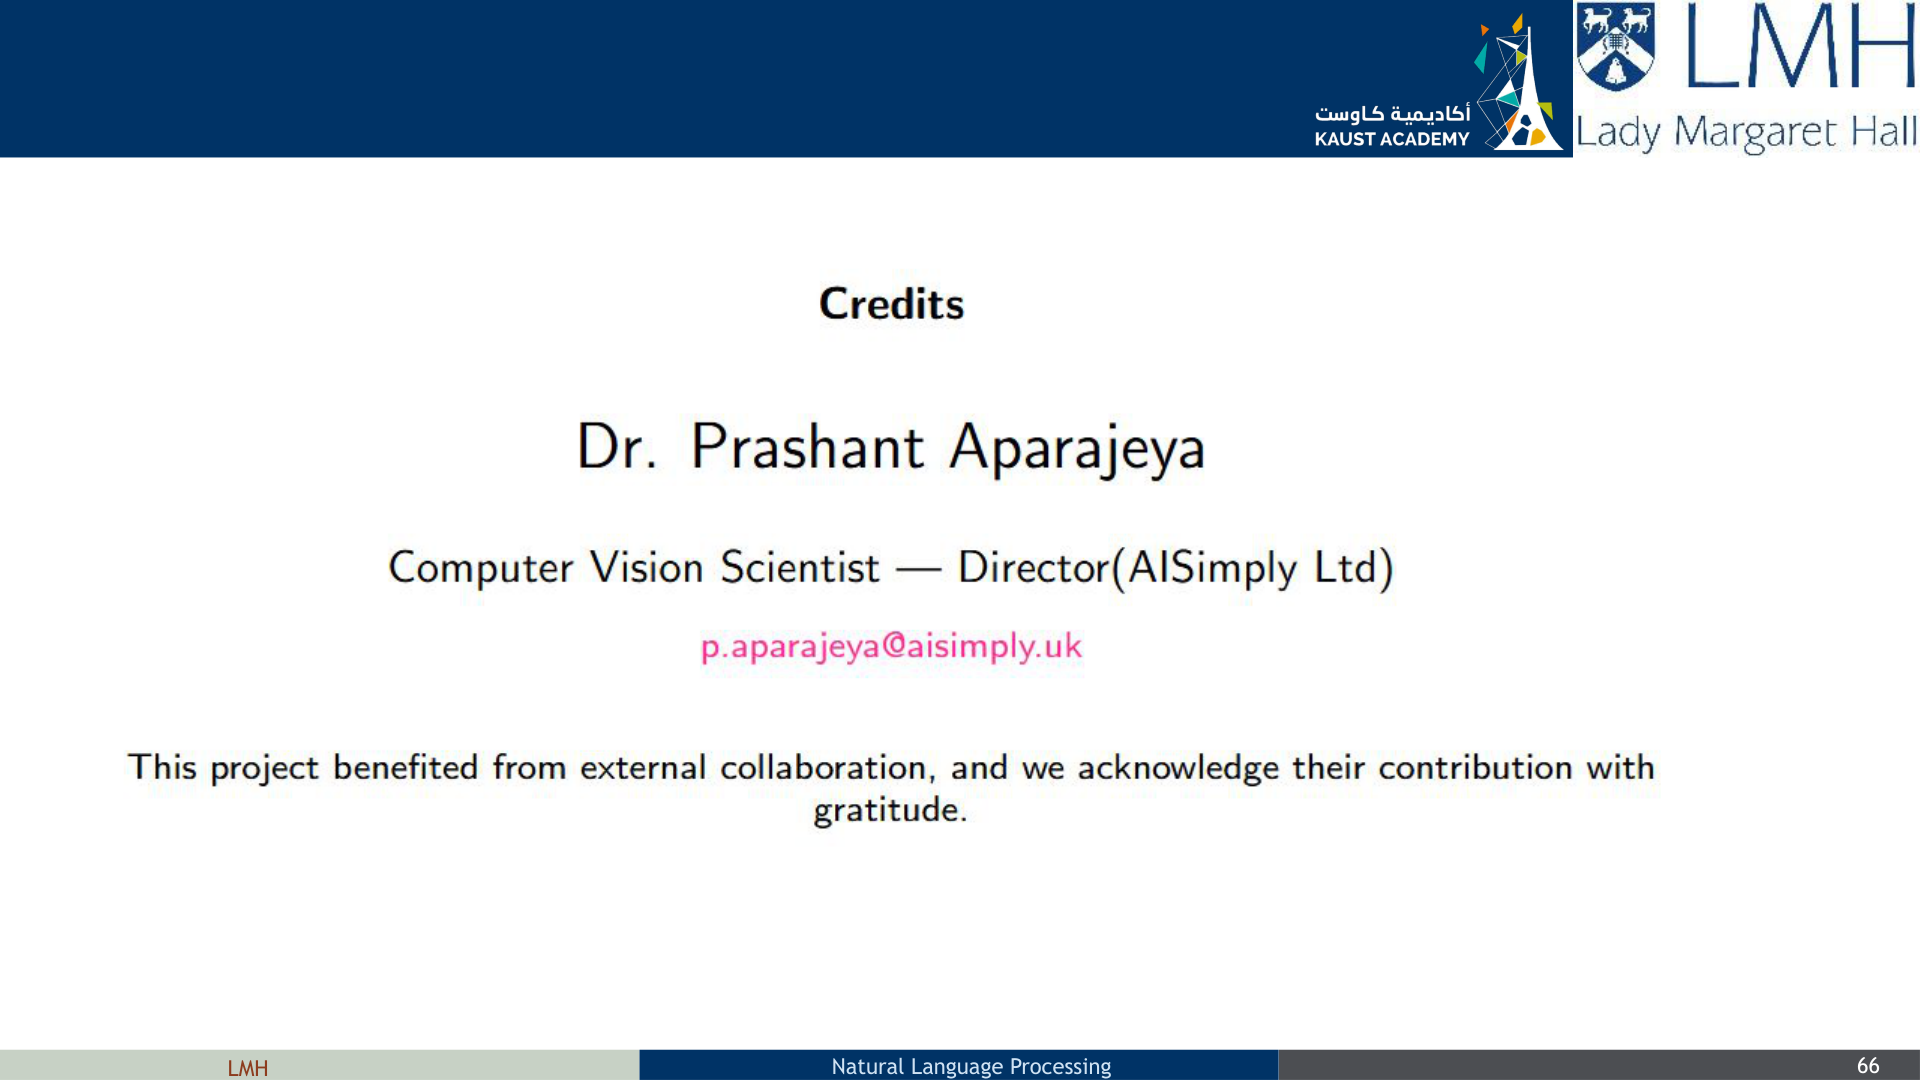
\includegraphics[width=\paperwidth,height=0.95\paperheight,keepaspectratio]{assets/Lecture-11_Large_Reasoning_Models_and_Mixture_of_Experts_Models/pdf_page_066.png}
\end{frame}

\end{document}
